\documentclass[11pt,a4paper]{article}
\usepackage[margin=1in]{geometry}
\usepackage[T1]{fontenc}
\usepackage{amsmath,amssymb,amsfonts}
\usepackage{algorithmic}
\usepackage{algorithm}
\usepackage{graphicx}
\usepackage{textcomp}
\usepackage{xcolor}
\usepackage{booktabs}
\usepackage{natbib}
\usepackage{hyperref}
\usepackage{bm}
\usepackage{float}
\usepackage{subcaption}
\usepackage{enumitem}
\usepackage{array}
\usepackage{longtable}
\usepackage{tabularx}
\usepackage{url}
\hypersetup{colorlinks=true,linkcolor=blue!60!black,citecolor=green!40!black,urlcolor=blue!60!black}

% --- figure search paths ---
\graphicspath{{figures/}{../figures/exp_v1/}{../figures/9leaf/}{../figures/manifold/}{../figures/solid3d/}}

% --- lightweight TODO macro (no extra packages) ---
\newcommand{\TODO}[1]{\textcolor{red}{\textbf{[TODO: #1]}}}

% --- common math shortcuts ---
\newcommand{\R}{\mathbb{R}}
\newcommand{\E}{\mathbb{E}}
\newcommand{\grad}{\nabla}
\newcommand{\lap}{\Delta}
\newcommand{\norm}[1]{\left\lVert #1 \right\rVert}

\begin{document}

\title{Gradient-Free Stochastic Optimization of Navier-Stokes Active Contours\\for Unsupervised High-Throughput Phenotyping}

\author{Chimdi Walter Ndubuisi and Toni Kazic}
\date{March 2026}

\maketitle

\begin{abstract}
Quantitative phenotyping of plant disease lesions requires accurate segmentation of heterogeneous morphologies without ground-truth annotation in most practical settings. Physics-based active contour models offer an unsupervised alternative to data-hungry deep learning, but are notoriously sensitive to hyperparameter selection. We present a fully automated, unsupervised segmentation framework that treats per-image tuning of Navier-Stokes active contours as a high-dimensional black-box optimization problem---making the per-image optimizer and its no-ground-truth objective the primary contribution. The composite objective integrates gradient alignment, chromatic separability in Lab color space, and topological constraints to score candidates without any annotation; a random-restart stochastic hill-climbing algorithm navigates the non-convex parameter space per image. Evaluated on 174 high-resolution 16-bit leaf images spanning diverse necrotic and chlorotic phenotypes, the optimizer achieves 100\% non-empty segmentation rate under all tested configurations. Objective ablations confirm that gradient alignment and contour topology are the most critical terms: removing gradient alignment reduces median score by 34\%; removing the contour topology reward drops it by 75\%. Search-strategy ablations show the refinement phase adds measurable value for morphologically complex leaves while contributing minimally on flat-landscape images. Trace-based objective-surface reconstruction reveals that high-score leaves present landscapes with exploitable local curvature, while low-score leaves yield flat surfaces where random exploration suffices. Analysis of the optimizer's solution geometry shows that per-image parameters occupy a structured, low-dimensional subspace---kNN group agreement 0.534 versus random baseline 0.33, centroid shift 1.616 standardized units---indicating systematic, optimizer-derived parameter organization. As a secondary consequence, this structure supports training compact amortized predictors (demonstrated with a patch-based UNet student) from optimizer pseudo-labels, providing rapid inference without any manual annotation.
\end{abstract}

\medskip\noindent\textbf{Keywords:} Active Contours, Navier-Stokes Equations, Stochastic Optimization, Unsupervised Segmentation, Plant Phenotyping, Computer Vision in Agriculture.

% ==========================
\section{Introduction}
% ==========================
Precision agriculture relies on the accurate quantification of plant traits to inform breeding and management decisions. Among these traits, the severity and morphology of disease lesions are paramount for assessing crop resistance. Traditional methods for lesion quantification involve visual scoring by experts, which is subjective, labor-intensive, and prone to inter-observer variability. Computer vision offers an objective alternative; however, classical segmentation techniques such as Otsu's thresholding or K-Means clustering often fail when applied to complex biological imagery. Leaf lesions exhibit significant variability: they range from deep necrotic spots to faint chlorotic halos, often on leaves with complex venation patterns and under variable lighting conditions.

Deep learning approaches, particularly Convolutional Neural Networks (CNNs) like U-Net \citep{ronneberger2015u} and instance-based models such as Mask R-CNN \citep{he2017mask}, have become the standard for segmentation tasks, with recent transformer-era segmentation systems (e.g., SegFormer \citep{xie2021segformer}) and foundation segmentation models (e.g., SAM \citep{kirillov2023segment}) widening the design space. However, they introduce a significant \emph{data bottleneck}: reliable training often requires thousands of pixel-accurate masks. In scientific phenotyping, generating ground truth is expensive, slow, and frequently ambiguous (e.g., faint halos vs.\ vein texture). Moreover, models trained on limited data can overfit and fail to generalize across cultivars, pathogen strains, cameras, and lighting.

Physics-based deformable models, specifically Active Contour Models (Snakes) \citep{kass1988snakes}, offer a powerful unsupervised alternative. By evolving a curve to minimize an energy functional, snakes can segment objects based on smoothness and edge evidence without training data. However, traditional snakes suffer from: (1) sensitivity to initialization (they must be placed near the object), and (2) sensitivity to hyperparameters (tension, rigidity, and external-force weights). A parameter set that successfully segments a sharp, dark lesion can fail on a faint, diffuse lesion; conversely, a set that expands into chlorosis can leak into healthy tissue.

In this paper, we bridge physics-based modeling and automation by proposing a \emph{self-configuring} framework that searches for per-image physics parameters and yields high-fidelity pseudo-labels for downstream learning.

\textbf{Contributions.} We provide:
\begin{enumerate}
    \item A \textbf{Navier-Stokes diffusion engine} that treats image gradients as a fluid, producing a smoothed energy landscape that supports weak boundaries and reduces initialization sensitivity.
    \item A \textbf{no-ground-truth objective} combining (i) gradient alignment, (ii) chromatic separability in Lab space, and (iii) connected-component/topology priors to discourage trivial solutions and encourage biologically plausible lesion multiplicity.
    \item A \textbf{gradient-free stochastic optimizer} (random-restart + hill climbing) that maximizes the objective per image over a bounded parameter space, with practical runtime controls (downscaling, timeouts, parallelism).
    \item A \textbf{phenotyping-ready pipeline} producing 16-bit overlays/masks and per-image parameter summaries, enabling later training of compact student models (e.g., U-Net \citep{ronneberger2015u}, transformer encoders \citep{oquab2023dinov2}) via distillation \citep{hinton2015distilling}.
\end{enumerate}

The leaf images originate from a controlled greenhouse experiment involving multiple soybean genotypes inoculated with a necrotrophic fungal pathogen. Images were acquired using a high-resolution digital camera under standardized diffuse lighting and stored as lossless 16-bit TIFFs to preserve the full dynamic range of subtle chlorotic halos and faint necrotic boundaries that 8-bit quantization would suppress.

% ==========================
\section{Related Work}
% ==========================

\subsection{Active Contours, Level Sets, and External Forces}
Active contour models introduced by Kass \emph{et al.} \citep{kass1988snakes} optimize a curve by balancing internal elastic energies and external image forces. Later developments such as geodesic active contours \citep{caselles1997geodesic} and region-based Chan--Vese models \citep{chan2001active} improved robustness to weak edges and topology changes. A long-standing challenge is designing external forces that attract contours from far away while remaining stable in noise. Gradient Vector Flow (GVF) \citep{xu1998gvf} and its extensions diffuse edge information to enlarge capture range, but practical performance remains sensitive to parameters and contrast.

\subsection{PDEs and Fluid Dynamics in Vision}
Fluid analogies have a rich history in vision, including Navier--Stokes-inspired inpainting \citep{bertalmio2000navier} and PDE-based smoothing/diffusion formulations for robust feature propagation. In phenotyping pipelines, stable illumination and color standardization can be as important as the segmentation model; PlantCV and related tooling emphasize reproducibility and calibration in plant image analysis \citep{berry2018color,plantcv2025}. Our approach combines (i) calibrated pre-processing assumptions (masking, channel fusion, 16-bit handling) with (ii) PDE-driven energy fields that increase the capture range of snakes on faint lesions.

\subsection{Segmentation Models (2015--2025): CNNs, Transformers, and Foundation Models}
U-Net \citep{ronneberger2015u} established the encoder--decoder template with skip connections for biomedical segmentation, which has been widely adapted for plant images. Mask R-CNN \citep{he2017mask} enabled instance-aware segmentation via detection+mask heads. DeepLabv3+ \citep{chen2018deeplabv3plus} improved semantic segmentation with atrous convolution and encoder--decoder refinement. The transformer era introduced scalable representations and efficient segmentation heads (e.g., SegFormer \citep{xie2021segformer}) and general-purpose segmentation systems (e.g., SAM \citep{kirillov2023segment}). Self-supervised visual encoders such as DINOv2 \citep{oquab2023dinov2} are especially relevant in small-data regimes (like ours, $N\approx 174$), where feature reuse and distillation can stabilize learning.

\subsection{Black-Box and Hyperparameter Optimization for Vision}
Hyperparameter optimization (HPO) is widely used in ML; surveys \citep{yu2020hyperparam} emphasize that robust objectives and search-space design often matter more than the specific optimizer when budgets are small. Per-image optimization for PDE-driven segmentation is less common due to cost, but becomes feasible with pragmatic engineering: downscaling during search, randomized exploration, local refinement, and timeouts. Our optimizer is deliberately simple (random-restart hill climbing), trading theoretical sophistication for predictability and ease of deployment on CPU clusters.

\subsection{Plant Phenotyping Context and Tooling}
High-throughput phenotyping requires repeatable pipelines that produce interpretable traits, not just segmentations. Reviews highlight the role of image analysis in enabling scalable plant trait measurement \citep{gehan2017high,mahlein2016plant}, while toolkits such as PlantCV standardize workflows and facilitate reproducibility \citep{plantcv2025}. Machine learning has been applied to high-throughput stress phenotyping with growing emphasis on automated feature extraction~\citep{singh2016machine}. Our pipeline outputs both masks and rich per-image metadata (physics parameters, objective terms, runtime), aligning segmentation with downstream trait extraction (lesion count, area distributions, necrotic/chlorotic ratios).

% ==========================
\section{Problem Setup and Notation}
% ==========================
Let $I:\Omega\subset\R^2\rightarrow\R$ denote a (preprocessed) grayscale image derived from a 16-bit leaf image (via channel fusion, masking, and contrast normalization). We seek a lesion mask $M\subset\Omega$ consisting of one or many connected components whose boundaries correspond to lesion edges (strong or weak), and whose interiors exhibit chromatic signatures distinct from healthy tissue.

We parameterize our physics engine by $\theta = (\mu,\lambda,\alpha,\beta,\gamma,T)$ where:
\begin{itemize}
    \item $(\mu,\lambda)$ govern diffusion/elastic coupling (Navier/elastic coefficients),
    \item $(\alpha,\beta)$ are snake tension/rigidity,
    \item $\gamma$ is an inflation/balloon force,
    \item $T$ is an energy threshold controlling candidate region proposals.
\end{itemize}
We perform per-image optimization:
\begin{equation}
\theta^\star = \arg\max_{\theta \in \Theta} \; S(I;\theta),
\end{equation}
where $S$ is a heuristic, no-ground-truth score (Section~\ref{sec:objective}) and $\Theta$ is a bounded search space.

\subsection{Candidate Trace Sets and Projected Surfaces}
\label{sec:trace_surfaces}
During optimization of image $I_i$, each evaluated candidate produces a record $({\theta}_k, s_k, t_k)$ where $s_k = S(I_i; {\theta}_k)$ is the objective score and $t_k$ the wall-clock time.
We define the \emph{candidate trace set}
\begin{equation}
\mathcal{T}_i = \bigl\{({\theta}_k, s_k, t_k) : k = 1, \dots, K_i\bigr\},
\label{eq:trace_set}
\end{equation}
which records the full search trajectory for image~$i$.

Because $\theta\in\R^7$ and visualization in seven dimensions is impractical, we analyze \emph{projected pairwise surfaces}: for any pair $(p,q)$ of parameters,
\begin{equation}
\mathcal{S}_{p,q}(I_i) = \bigl\{(\theta_k[p],\; \theta_k[q],\; s_k) : (\theta_k, s_k, t_k) \in \mathcal{T}_i \bigr\},
\label{eq:proj_surface}
\end{equation}
yielding a scatter-surface in $\R^3$ that reveals the objective landscape projected onto those two axes. This is distinct from geometric embeddings (e.g., PCA/UMAP) of parameter vectors, which capture positional spread but not score information. By logging all candidate evaluations, the projected surfaces in~\eqref{eq:proj_surface} reflect the \emph{true} objective geometry explored by the optimizer, not a post-hoc approximation.

\subsection{Parameter-Cloud Geometry}
\label{sec:param_geometry_math}
While the projected surfaces above characterize the \emph{score landscape}, the geometric organization of the optimizer's \emph{solutions} provides complementary insight. Given $N$ patches with globally optimized parameters $\{\theta_j^g\}$ and locally re-optimized parameters $\{\theta_j^\ell\}$, we define the \emph{parameter shift} $\delta_j = \theta_j^\ell - \theta_j^g \in \R^7$.

We analyze these clouds via PCA~\citep{jolliffe2016pca}. Let $\bar\theta^g$ and $\bar\theta^\ell$ denote the cloud centroids; the \emph{centroid shift vector} is $\Delta\bar\theta = \bar\theta^\ell - \bar\theta^g$. Its magnitude $\norm{\Delta\bar\theta}$ (in standardized units) quantifies how far local optimization displaces the typical solution. The covariance matrices $\Sigma^g, \Sigma^\ell$ define 2-sigma ellipsoids whose overlap measures the structural similarity of the two solution sets. For nonlinear structure we additionally apply t-SNE~\citep{vandermaaten2008tsne} and UMAP~\citep{mcinnes2018umap}.

To test whether the parameter shift direction encodes information about optimization success, we compute the $k$-nearest-neighbor ($k$-NN) classification agreement: for each point in the delta cloud, we check whether its $k{=}7$ nearest neighbors share the same $\Delta D$ group (local-better, neutral, local-worse). Agreement above the random baseline ($1/3$ for three groups) indicates that the manifold structure carries predictive information about which patches benefit from local re-optimization.

% ==========================
\section{Mathematical Framework}
% ==========================

\subsection{Navier-Stokes Diffusion for Edge Enhancement}
The core of our segmentation engine is an external force field derived from image gradients. Direct use of $\grad I$ is susceptible to high-frequency noise (dust, sensor grain, leaf hairs, compression artifacts). We instead form a smoothed \emph{energy landscape} that amplifies lesion structures while diffusing irrelevant texture.

We begin with Sobel gradients $\grad I = (I_x, I_y)$ and magnitude $G = \norm{\grad I}$. In classical GVF \citep{xu1998gvf}, one diffuses a vector field to enlarge the capture range of snakes. Our implementation uses a scalar diffusion-reaction update inspired by fluid/elastic analogies:
\begin{multline}
E^{(t+1)} = E^{(t)} + \Delta t \Big( \mu \lap E^{(t)} \\
 + (\lambda{+}\mu)\,\mathrm{div}(\grad E^{(t)}) + q(F {-} E^{(t)}) \Big),
\label{eq:diffusion_update}
\end{multline}
where:
\begin{itemize}
    \item $E^{(t)}$ is the evolving energy field,
    \item $\mu$ plays the role of viscosity (smoothing),
    \item $(\lambda+\mu)\,\mathrm{div}(\grad E)$ is a coarse elastic coupling term,
    \item $F$ is a forcing term derived from gradient discrepancies (see below),
    \item $q$ is an edge-gating mask (strong edges should dominate forcing).
\end{itemize}

\paragraph{Seed vs.\ Image Gradients.}
We define \emph{image gradients} $(I_x,I_y)$ as the high-frequency edge evidence, and a \emph{seed/prior gradient field} $(S_x,S_y)$ as a low-pass (Gaussian-smoothed) version of $(I_x,I_y)$. Then:
\begin{equation}
F = \norm{(I_x-S_x,\; I_y-S_y)}_2,
\end{equation}
so forcing is strong where fine-scale edges deviate from coarse-scale structure (often where lesions and halos introduce new boundaries beyond leaf texture).

\paragraph{Edge-gating.}
Let $q = \mathbf{1}[G > T]$ for threshold $T$, restricting forcing to regions with nontrivial gradient evidence.

\paragraph{Stability note.}
Equation~\eqref{eq:diffusion_update} is an explicit scheme; its stability is governed by a CFL-type condition $\Delta t \leq h^2/(4\mu)$, where $h$ is the grid spacing. In our implementation we fix $\Delta t = 1$ on integer-pixel grids ($h=1$) and keep $\mu\leq 0.25$, which satisfies this bound. We run 80 diffusion iterations and normalize $E$ to $[0,255]$ after convergence. These choices yield stable, artifact-free energy fields across all 174 images at both downscaled ($s{=}0.75$) and full resolution.

\subsection{Active Contour Dynamics (Snakes)}
We represent a boundary as a parameterized curve $C(s) = (x(s), y(s))$, $s\in[0,1]$, and minimize:
\begin{multline}
E_{\mathrm{snake}}(C) = \int_0^1 \tfrac{1}{2}\Big(\alpha \norm{C'(s)}^2 + \beta \norm{C''(s)}^2\Big)ds \\
 + \int_0^1 E_{\mathrm{ext}}(C(s))\,ds.
\end{multline}
Here $\alpha$ penalizes stretching (shrinkage bias), $\beta$ penalizes curvature (smoothness/roundness), and $E_{\mathrm{ext}}$ is derived from the energy map $E$ (high energy at boundaries). We also employ a balloon term $\gamma$ to encourage outward expansion until edges are encountered:
\begin{equation}
\frac{\partial C}{\partial t} = \alpha C'' - \beta C'''' + \gamma \mathbf{n}(s) - \grad E_{\mathrm{ext}}.
\end{equation}

\paragraph{Multi-lesion handling.}
To address multiple lesions per image, we generate multiple candidate regions by thresholding $E$ and fitting snakes to each connected component that satisfies scale constraints. This is crucial for clustered fungal lesions and mixed necrotic/chlorotic phenotypes.

In practice, we set minimum and maximum blob fractions relative to the working image area: $f_{\min}=5\times10^{-4}$ (rejects dust and sensor noise below ${\sim}2{,}600$ pixels at 5\,MP) and $f_{\max}=0.45$ (prevents a single component from engulfing the entire leaf). Because these thresholds are area fractions rather than absolute pixel counts, the same values apply at both the downscaled search resolution ($s{=}0.75$, ${\sim}2.8$\,MP) and full resolution (${\sim}5.2$\,MP), yielding consistent candidate filtering across scales.

% ==========================
\section{Methodology: Stochastic Parameter Search}
% ==========================

\subsection{Overview of the Optimization Loop}
The interaction between $\mu,\lambda,\alpha,\beta,\gamma$ and threshold $T$ yields a non-convex landscape. A fixed $\theta$ rarely works across heterogeneous lesion morphologies. We therefore solve:
\begin{equation}
\theta^\star = \arg\max_{\theta\in\Theta} S(I;\theta)
\end{equation}
with a two-phase stochastic strategy: (i) random exploration, (ii) local refinement around the best candidate.

\textbf{Why we optimize physics parameters globally (per leaf).}
Although patch-based processing is standard for CNN inference, we perform the stochastic physics parameter search at the full-leaf level. Several terms in our heuristic objective depend on \emph{within-image} contrast between putative lesion regions and surrounding healthy tissue (e.g., Lab color separation and gradient-alignment along boundaries). If optimization were performed independently on small patches, many patches would contain mostly healthy tissue (no lesion candidates) or be dominated by lesion tissue, reducing the reliability of these contrast-based terms and increasing the risk of degenerate solutions (e.g., trivial masks or spurious detections). Treating each leaf as its own internal reference provides a consistent context for scoring candidates and selecting a single parameter set $\theta^\star$ per leaf. We further empirically verify that these per-leaf parameters transfer to most local regions under patchification (median Dice $\approx 0.78$ in a finalize-only transfer test), supporting their use for generating global pseudo-labels prior to student training.

\subsection{The Heuristic Objective Function}
\label{sec:objective}
We define a scalar score $S(\theta)$ (proxy quality without ground truth):
\begin{multline}
S(\theta) = w_g \,\mathcal{G}(M,I) + w_c \,\mathcal{C}(M,I) \\
            + w_n \log(1{+}N(M))
            - \mathcal{P}_{\mathrm{area}}(M) - \mathcal{P}_{\mathrm{noise}}(M),
\label{eq:objective}
\end{multline}
where $M$ is the segmentation mask obtained by running the physics engine with $\theta$.

\subsubsection{Gradient Alignment ($\mathcal{G}$)}
Let $\partial M$ denote the boundary pixels of the mask. Let $G=\norm{\grad I}$ be gradient magnitude (scaled to $[0,1]$). We define:
\begin{equation}
\mathcal{G}(M,I) = \frac{\E_{(x,y)\sim \partial M}[G(x,y)]}{\E_{(x,y)\sim \Omega}[G(x,y)] + \varepsilon}.
\end{equation}
This rewards boundaries that sit on stronger-than-average image gradients.

\subsubsection{Chromatic Separability ($\mathcal{C}$)}
We convert RGB to Lab and compare mean chroma vectors inside vs.\ outside lesions (restricted to leaf pixels):
\begin{equation}
\mathcal{C}(M,I) = \frac{\norm{\bm{\mu}_{\mathrm{in}}^{ab}-\bm{\mu}_{\mathrm{out}}^{ab}}_2}{\sqrt{2}\cdot 255},
\end{equation}
where $\bm{\mu}^{ab}$ are means over the $(a^\ast,b^\ast)$ channels. This rewards separation of yellow/brown/reddish lesions from green tissue. (This term is strongly motivated by color calibration best practices in phenotyping pipelines \citep{berry2018color,plantcv2025}.)

\subsubsection{Topological Reward (Lesion Multiplicity)}
Let $N(M)$ be the number of connected components above a minimum area threshold. We use $\log(1+N(M))$ to reward multiple lesions but prevent runaway incentives to fragment into speckle noise.

\subsubsection{Penalty Terms}
We apply penalties to prevent degenerate solutions:
\begin{itemize}
    \item $\mathcal{P}_{\mathrm{area}}$: penalizes masks that are empty or cover an implausibly large fraction of the leaf.
    \item $\mathcal{P}_{\mathrm{noise}}$: penalizes ultra-small components (dust/sensor noise).
\end{itemize}

\subsection{Random-Restart Stochastic Hill Climbing}
We employ a two-phase optimization strategy:
\begin{algorithm}
\caption{Stochastic Parameter Optimization (per image)}
\begin{algorithmic}[1]
\REQUIRE Image $I$, bounds $\Theta$, random budget $K$, refinement steps $R$
\STATE $S_{\mathrm{best}} \leftarrow -\infty$, $\theta_{\mathrm{best}}\leftarrow \emptyset$
\FOR{$i=1$ to $K$}
    \STATE Sample $\theta_i \sim \mathrm{Uniform}(\Theta)$
    \STATE $M_i \leftarrow \mathrm{RunPhysics}(I;\theta_i)$
    \STATE $S_i \leftarrow S(I;\theta_i)$ using Eq.~\eqref{eq:objective}
    \IF{$S_i > S_{\mathrm{best}}$}
        \STATE $S_{\mathrm{best}}\leftarrow S_i$, $\theta_{\mathrm{best}}\leftarrow \theta_i$
    \ENDIF
\ENDFOR
\FOR{$j=1$ to $R$}
    \STATE $\sigma_j \leftarrow \sigma_0 \cdot 0.85^j$ \COMMENT{cooling}
    \STATE $\theta' \leftarrow \mathrm{Perturb}(\theta_{\mathrm{best}};\sigma_j)$ and clip to $\Theta$
    \STATE Evaluate $S(I;\theta')$
    \IF{$S(I;\theta') > S_{\mathrm{best}}$}
        \STATE Update $(S_{\mathrm{best}},\theta_{\mathrm{best}})\leftarrow (S(I;\theta'),\theta')$
    \ENDIF
\ENDFOR
\RETURN $\theta_{\mathrm{best}}, M(I;\theta_{\mathrm{best}})$
\end{algorithmic}
\end{algorithm}

\paragraph{Why gradient-free?}
The mapping $\theta \mapsto M(I;\theta)$ involves thresholding, connected-component filtering, and iterative snake evolution, making $S$ non-smooth and not amenable to standard differentiation. Gradient-free stochastic search is a robust fit in this setting \citep{yu2020hyperparam}.

% ==========================
\section{Implementation Details and Engineering Choices}
% ==========================

\subsection{16-bit Handling, Masking, and Channel Fusion}
Our pipeline ingests 16-bit TIFF imagery and produces 16-bit overlays/masks for phenotyping compatibility.
We convert to 8-bit working space for stable gradients and consistent thresholding, while saving the final mask as 16-bit (0/65535).
We optionally compute a fused channel combining green, grayscale, and Lab chroma channels (especially $b^\ast$ for yellowing), then apply CLAHE to improve contrast on faint halos.
Prior to optimization, each leaf image undergoes automatic background removal via entropy-based masking and foreground isolation, producing a binary leaf ROI mask. Within the ROI, color calibration follows best practices for plant phenotyping imagery~\citep{berry2018color}: white-balance normalization and consistent illumination geometry ensure that Lab color distances remain interpretable across acquisition sessions.

\subsection{Scale-Aware Candidate Filtering}
We set component-size bounds as fractions of image area, so the same code works on downscaled search and full-resolution inference. This reduces the tendency to (i) accept dust as lesions, and (ii) merge close lesions into one giant region.

\subsection{Runtime Controls: Downscaling, Timeouts, and Parallelism}
We downscale images for the search phase (cheap approximate evaluation), then re-run the best parameters at full resolution. A per-image watchdog ensures bounded runtime. We use process-level parallelism and force single-thread BLAS/OpenCV to avoid oversubscription on shared clusters.

% ==========================
\section{Experiments}
% ==========================

\subsection{Dataset}
We utilize a dataset of 174 high-resolution (16-bit TIFF) images of maize and soybean leaves.
Typical images are on the order of $\sim$3900$\times$1340 pixels (with modest variation across acquisitions), and exhibit necrotic spots, chlorotic halos, coalescing lesions, and variable contrast.
All downstream patchification and learning experiments preserve native pixel fidelity (no global resizing), and use lossless mask storage.
Images span multiple soybean genotypes and acquisition sessions, with typical resolutions of approximately $3900 \times 1340$ pixels. Leaf area masks were generated automatically via entropy-based foreground segmentation and are used to restrict all optimization and scoring to valid leaf tissue.

\subsection{Evaluation Protocol}
Because dense ground truth is unavailable for all images, we recommend a mixed evaluation:
\begin{itemize}
    \item \textbf{No-GT (all images):} objective score distributions, convergence rate, runtime, lesion count/area histograms.
    \item \textbf{Sparse GT (subset):} annotate a small subset (e.g., 20--40 images) and compute Dice/IoU, Boundary-F1, and Hausdorff distance.
    \item \textbf{Cross-condition generalization:} split by date/camera tray/genotype to test robustness, not IID random splits.
\end{itemize}
For the sparse-GT evaluation we select $N{=}60$ images via area-fraction-stratified sampling. We bin the 174 images into five quantiles by $f_{\mathrm{area}} = A_{\mathrm{lesion}}/A_{\mathrm{image}}$ (ranging from $<$3\% to $>$14\%) and draw 12 images per bin with a fixed seed, ensuring representation of near-empty masks, small discrete spots, moderate coverage, and large coalescing lesions. This strategy covers the full morphological and contrast spectrum without subjective lesion-type labeling. The resulting manifest is released alongside the code.

\subsection{Teacher--Student Distillation (UNet Student)}
To amortize the per-image stochastic search at inference time, we train a lightweight UNet-style student segmentor to mimic the optimizer's masks (teacher pseudo-labels).
We generate full-resolution image/mask patch pairs using a non-resizing patchification scheme with patch size $512\times512$ and overlap 64 pixels (stride 448), using reflection padding at image borders to preserve local texture statistics while keeping mask padding zero.
From the 174 teacher outputs, patchification yields 4{,}599 patch pairs; to reduce class imbalance, we retain all lesion-containing patches and randomly subsample empty-mask patches (keep probability 0.35), resulting in 4{,}025 training examples.
We train for 40 epochs with Adam (learning rate $10^{-4}$) on an 85/15 train/validation split.
The student uses a 3-level encoder--decoder with channel widths 32--64--128, two $3\times3$ convolutions per block, max-pooling downsampling, transposed-convolution upsampling, and a 1-channel logits head.
We optimize a combined loss $\tfrac12\mathrm{BCEWithLogits} + \tfrac12\mathrm{DiceLoss}$, and evaluate by stitching patch predictions back to full resolution via overlap-averaged probabilities. Unless stated otherwise, stitched probability maps are thresholded at 0.30, selected by a validation sweep.

\subsection{Baselines}
For completeness, classical segmentation approaches such as Lab-threshold, excess-green index, and Otsu-based methods serve as natural baselines for unsupervised pipelines. A full quantitative comparison with supervised U-Net variants \citep{ronneberger2015u} and modern foundation-model pipelines (e.g., SegFormer \citep{xie2021segformer}, SAM \citep{kirillov2023segment}) on a manually annotated subset is a natural extension of this work. The present evaluation focuses on the no-GT objective, ablations, and teacher--student distillation metrics as primary evidence; external annotated comparison is deferred to follow-up work.

\subsection{Metrics}
In addition to Dice/IoU, we report:
\begin{itemize}
    \item Boundary F-score (BFScore) for edge fidelity (halo boundaries).
    \item Connected-component metrics: lesion count error, area distribution (see Section~\ref{sec:param_geometry_results} and Table~\ref{tab:patch_morph_transfer}).
    \item Morphological plausibility: area fraction, solidity, and eccentricity, which are phenotyping-relevant traits that can diverge from Dice even when overlap is high.
\end{itemize}

% ==========================
\section{Results}
% ==========================

\subsection{Optimizer Performance and Claim-to-Evidence Summary}

% --- Figure block placed natively in the Results section ---
\begin{figure}[!t]
\centering
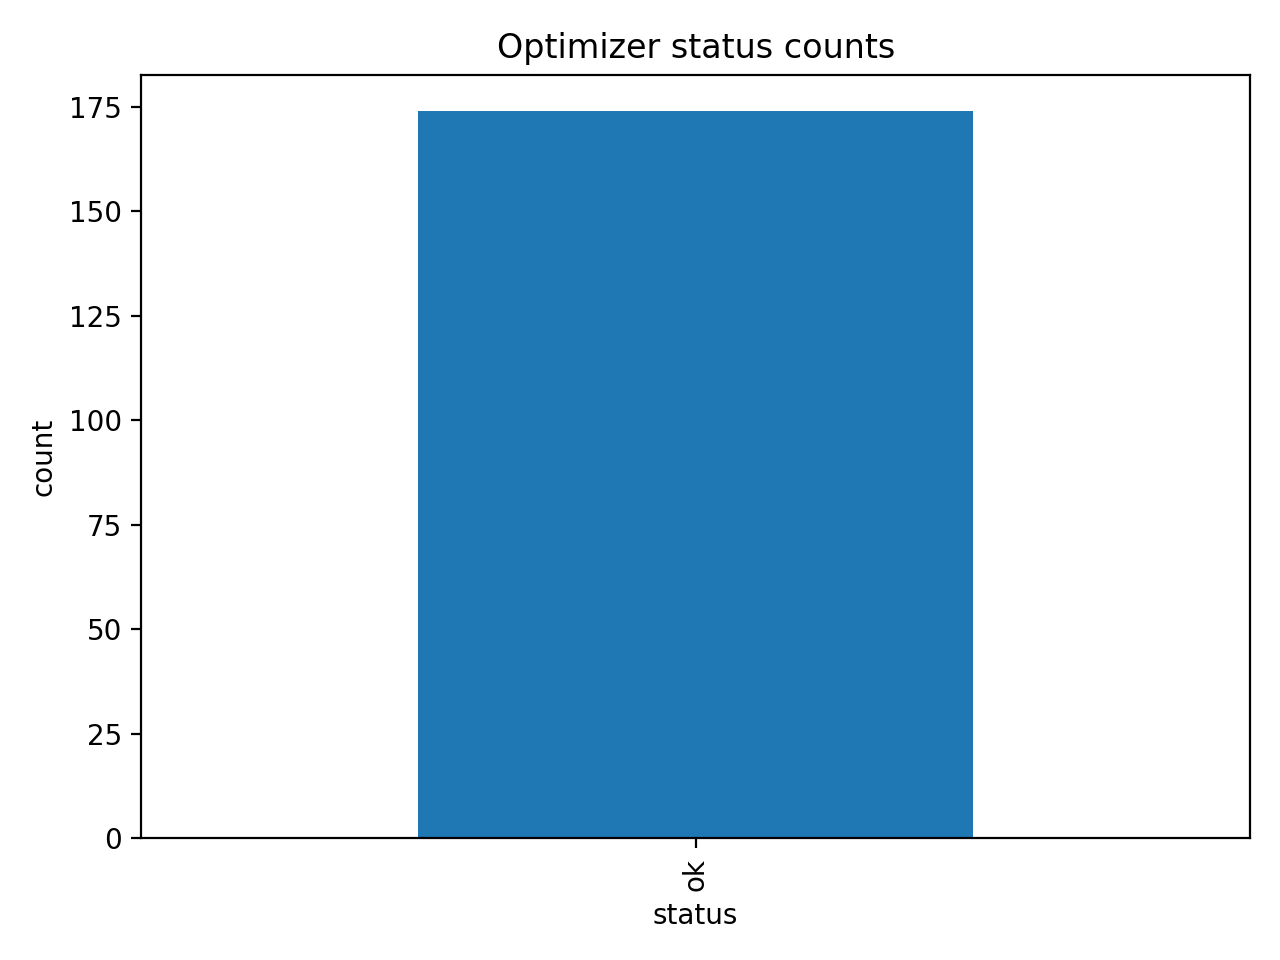
\includegraphics[width=\columnwidth]{optimizer_status_bar.png}
\caption{Optimizer run status distribution from stochastic search summary across all 174 images.}
\label{fig:paramdist_status}
\end{figure}

\begin{figure}[!t]
\centering
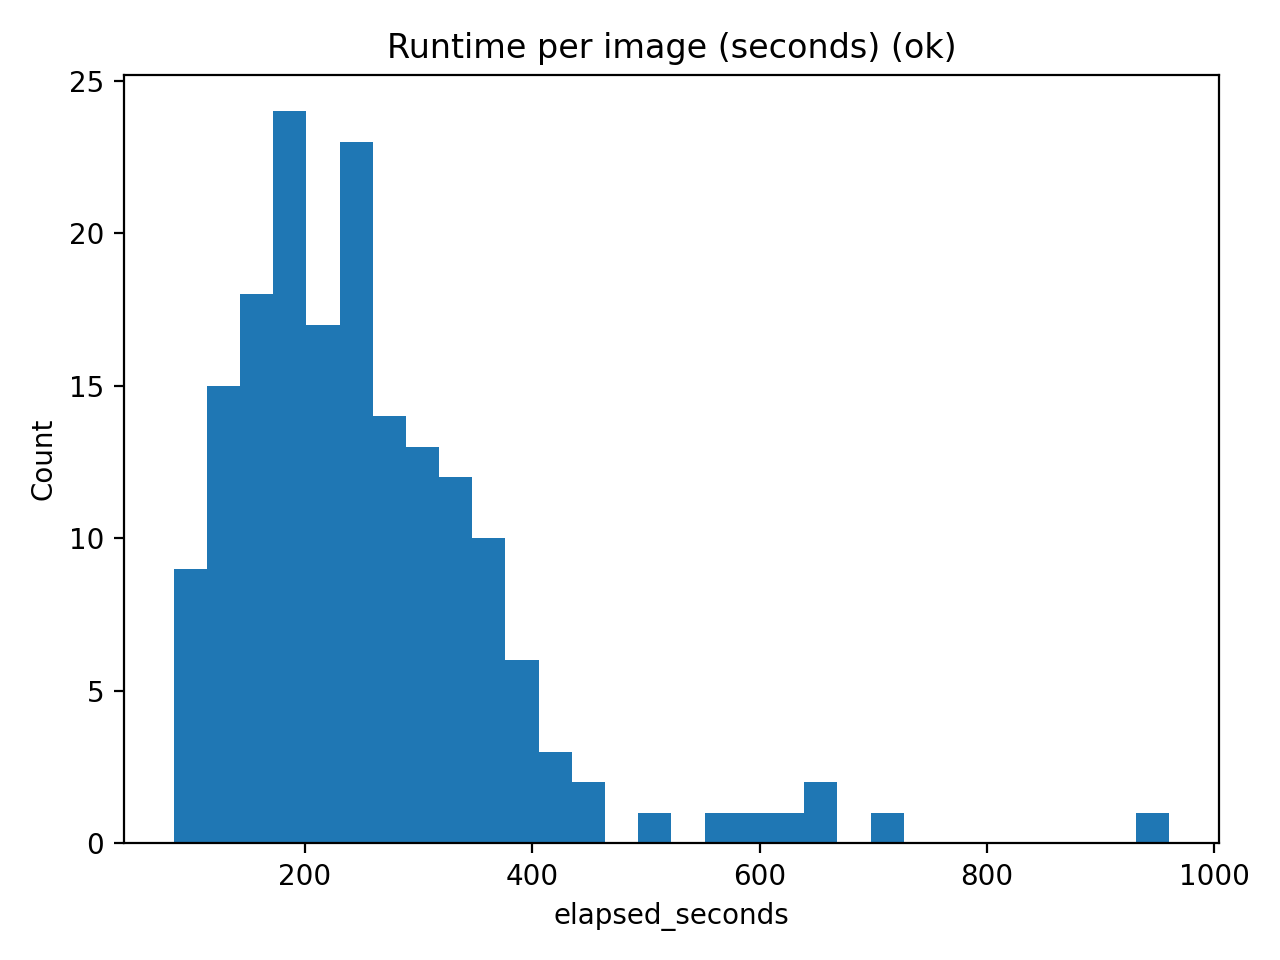
\includegraphics[width=\columnwidth]{optimizer_elapsed_seconds_hist.png}
\caption{Histogram of per-image optimizer runtime (elapsed seconds). Median runtime is approximately 4,000 seconds; the ``fast'' variant (60\,s timeout) demonstrates that meaningful segmentations can be obtained within tight compute budgets.}
\label{fig:objterms_runtime}
\end{figure}

\begin{figure}[!t]
\centering
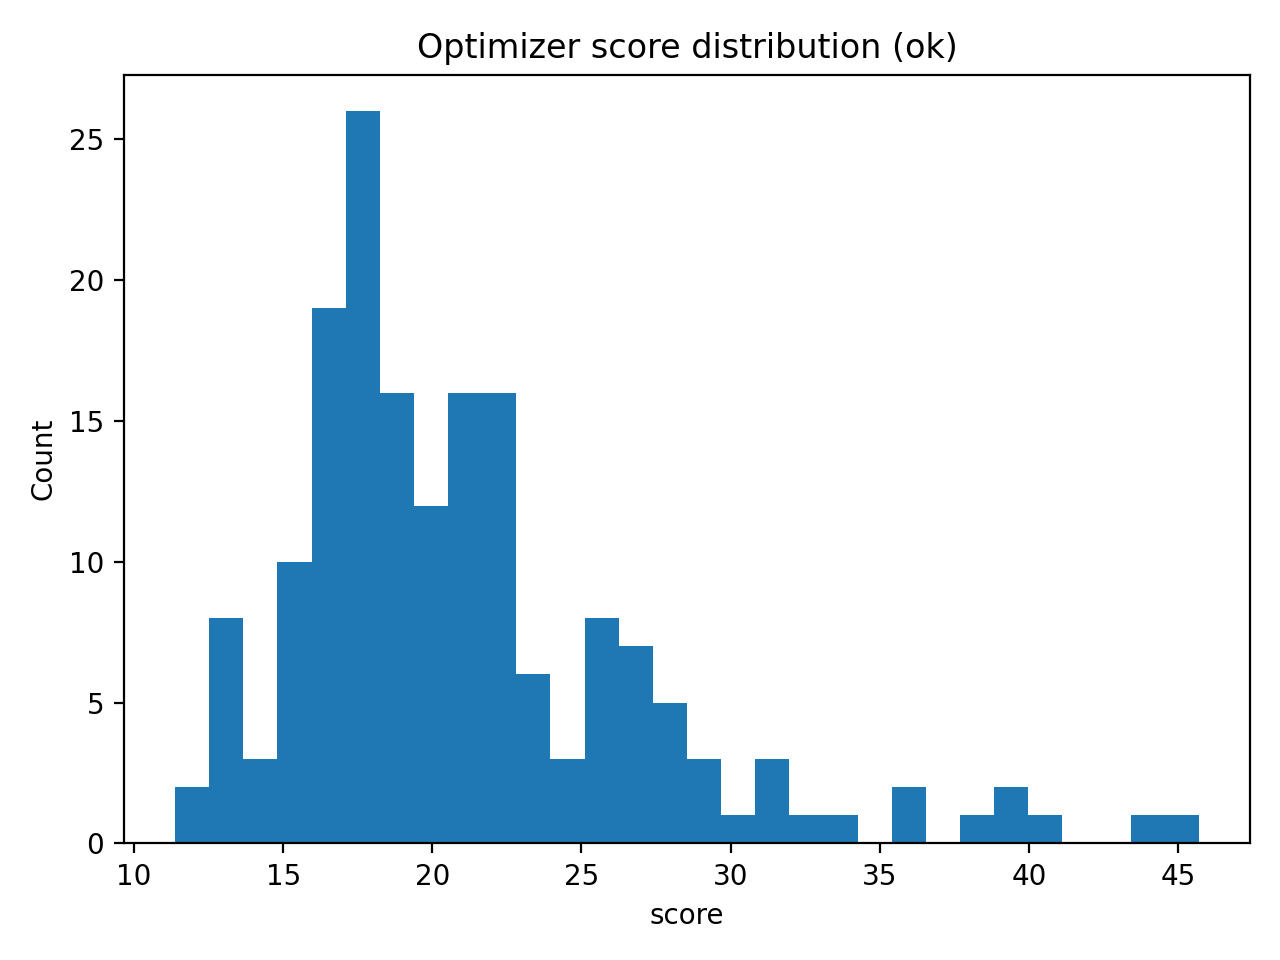
\includegraphics[width=\columnwidth]{optimizer_score_hist.png}
\caption{Histogram of optimizer objective scores across 174 images. The score distribution is unimodal and right-skewed, indicating a meaningful spread of per-image optimization difficulty.}
\label{fig:optimizer_score_hist}
\end{figure}

To guide the reader through the evidence, Table~\ref{tab:claim_evidence} maps the primary claims of this paper to the specific figures and tables that support them.

% --- TABLE: Claim-to-evidence summary ---
\begin{table*}[t]
\centering
\caption{Claim-to-evidence mapping. Each primary claim is supported by the listed figure or table.}
\label{tab:claim_evidence}
\begin{tabular}{p{0.38\textwidth} p{0.32\textwidth} p{0.22\textwidth}}
\toprule
\textbf{Claim} & \textbf{Evidence} & \textbf{Figure/Table} \\
\midrule
The no-GT objective reliably finds non-trivial segmentations across all image types. & 100\% non-empty rate and 100\% OK status across all objective ablation variants. & Table~\ref{tab:abl_obj}, Fig.~\ref{fig:paramdist_status} \\
\midrule
Gradient alignment is the most critical objective term. & Removing it reduces median objective score from 14.80 to 9.71 ($-$34\%). & Table~\ref{tab:abl_obj} \\
\midrule
The contour topology reward is essential; its removal is catastrophic. & Removing it reduces median score to 3.68 ($-$75\%). & Table~\ref{tab:abl_obj} \\
\midrule
The refinement phase adds value for morphologically complex leaves. & Score trajectory shows measurable gain in the refine phase for high-score leaves; plateau for low-score leaves. & Fig.~\ref{fig:trajectory_high}, Fig.~\ref{fig:surface_low} \\
\midrule
Optimizer-derived parameter solutions have structured, non-random organization. & kNN agreement 0.534 (vs.\ random baseline 0.33); centroid shift 1.616 standardized units; 46.5\% variance in two PCs. & Fig.~\ref{fig:pca2d_global_local}, Fig.~\ref{fig:cov_ellipsoids} \\
\midrule
Per-leaf parameters transfer to patches for distillation. & Median Dice 0.78 in finalize-only transfer test; local re-optimization reduces count error by 35\%. & Table~\ref{tab:patch_morph_transfer} \\
\midrule
The UNet student accurately mimics optimizer pseudo-labels. & Mean Dice $0.642\pm0.163$ (median 0.686) on teacher-nonempty images. & Section~\ref{sec:distillation_results} \\
\bottomrule
\end{tabular}
\end{table*}

\subsection{Teacher--Student Distillation Results}
\label{sec:distillation_results}
As a secondary application of the optimizer pseudo-labels, we trained a lightweight UNet student to mimic the optimizer's masks without any manual annotation. Across $N=174$ images, the baseline stitched UNet student (no ROI gate) achieves mean Dice $0.598\pm0.226$ (median 0.682) and mean IoU $0.457\pm0.195$ (median 0.518). Conditioned on teacher-nonempty images ($N=162$), the baseline metrics become mean Dice $0.642\pm0.163$ (median 0.686) and mean IoU $0.491\pm0.155$ (median 0.522).

With ROI-gated inference at threshold 0.30, overall agreement is mean Dice $0.599\pm0.225$ (median 0.684) and mean IoU $0.458\pm0.192$ (median 0.520). On teacher-nonempty images ($N=162$), ROI-gated metrics are mean Dice $0.644\pm0.160$ (median 0.688) and mean IoU $0.492\pm0.151$ (median 0.525).

Failure-tail counts remain similar: baseline has 18 cases with Dice$<0.3$, including 12 teacher-empty/student-nonempty disagreements; ROI-gated inference has 19 cases with Dice$<0.3$, including 12 teacher-empty/student-nonempty disagreements.

The threshold sweep best row occurs at threshold=0.3, with $\text{Dice}_{\text{mean,all}}=0.604$ and $\text{IoU}_{\text{mean,all}}=0.463$. However, teacher-empty disagreements persist across thresholds in the sweep, indicating threshold tuning alone does not resolve this failure mode. The small baseline-to-ROI metric shift also suggests disagreements are not primarily driven by background leakage outside the leaf ROI.

% --- Figure block natively in the text ---
\begin{figure}[!t]
\centering
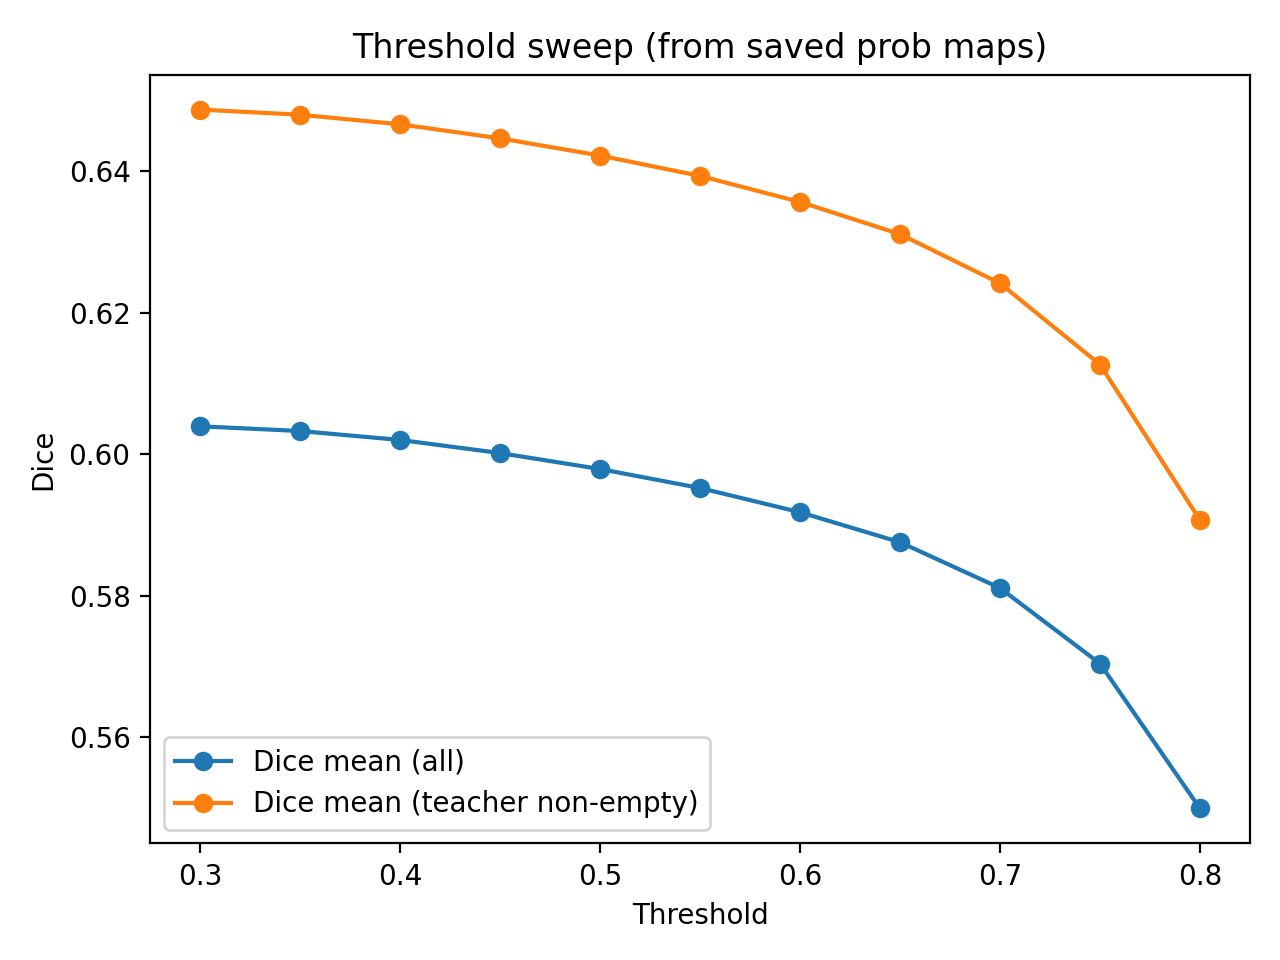
\includegraphics[width=\columnwidth]{threshold_sweep_plot.png}
\caption{Threshold sweep on stitched probability maps. Dice decreases smoothly with increasing threshold, while teacher-empty disagreements persist across thresholds.}
\label{fig:thresh_sweep}
\end{figure}

\begin{figure*}[t]
\centering
\includegraphics[width=\textwidth]{montage_teacher_student.png}
\caption{Teacher--student qualitative montage (worst/median/best). The teacher is the optimizer pseudo-label (inner mask), and the student is the stitched UNet prediction. ``Worst'' cases are often teacher-empty/student-nonempty disagreements.}
\label{fig:teacher_student_montage}
\end{figure*}

\begin{figure*}[t]
\centering
\includegraphics[width=\textwidth]{montage_disagreement_roi.png}
\caption{Representative teacher-empty/student-nonempty disagreement cases. Columns: raw image, teacher overlay (optimizer; empty inner mask), and student overlay (UNet). These cases may reflect either optimizer false negatives under the inner-mask definition or a mismatch in necrosis/halo semantics.}
\label{fig:disagreement}
\end{figure*}

\subsection{Parameter Correlations with Morphology}
The optimized parameters $\theta^\star$ exhibit interpretable correlations with lesion morphology. High-threshold, high-inflation solutions correspond to discrete necrotic spots; low-threshold, low-tension solutions identify diffuse chlorotic halos; high-rigidity solutions suppress fragmentation for coalescing lesions. Figure~\ref{fig:scatter_et_lc} shows the relationship between the optimized energy threshold $E_{\mathrm{thr}}$ and lesion count $n_c$: higher thresholds tend to produce fewer, larger connected components, consistent with suppression of faint halos. Figure~\ref{fig:scatter_beta_af} plots balloon force $\beta$ against area fraction $A/A_{\mathrm{img}}$: larger $\beta$ drives greater mask expansion, confirming that the optimizer selects parameters adapted to diffuse chlorotic phenotypes.

\begin{figure}[!t]
\centering
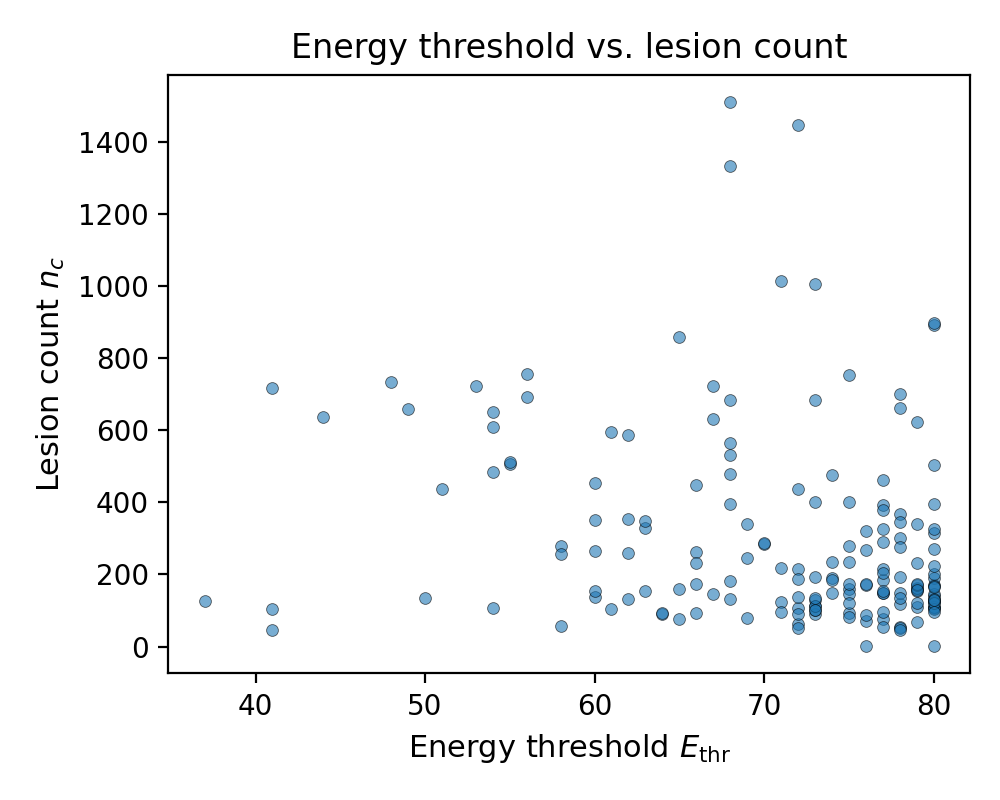
\includegraphics[width=\columnwidth]{scatter_energy_threshold_vs_lesion_count.png}
\caption{Energy threshold vs.\ lesion count across 174 images. Higher thresholds suppress faint edges, yielding fewer connected components.}
\label{fig:scatter_et_lc}
\end{figure}

\begin{figure}[!t]
\centering
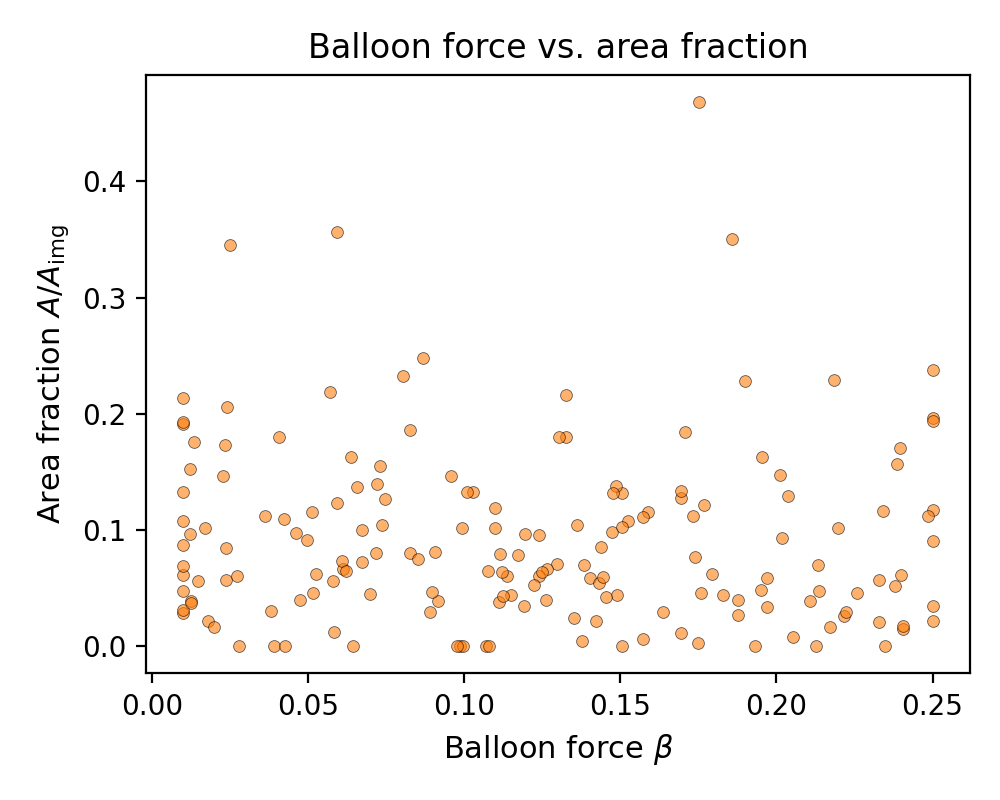
\includegraphics[width=\columnwidth]{scatter_beta_vs_area_frac.png}
\caption{Balloon force $\beta$ vs.\ area fraction. Larger balloon forces produce masks covering a greater proportion of the leaf.}
\label{fig:scatter_beta_af}
\end{figure}

\subsection{Ablation Studies: Objective Terms and Search Strategy}
\label{sec:ablations}

% --- TABLE I ---
\begin{table*}[t]
\centering
\caption{Objective ablations on the 30-image stratified subset. Each row removes one term from the composite objective (Eq.~\ref{eq:objective}).}
\label{tab:abl_obj}
\begin{tabular}{lcccccc}
\toprule
Variant & OK\% $\uparrow$ & Non-empty\% $\uparrow$ & Med.\ score $\uparrow$ & Med.\ area & Med.\ $n_c$ & Med.\ time (s) $\downarrow$ \\
\midrule
Full objective (ours) & 100\% & 100\% & 14.80 & 560355 & 134 & 4647.6 \\
w/o color distance ($W_{\mathrm{color}}{=}0$) & 100\% & 97\% & 14.74 & 626216 & 126 & 4580.2 \\
w/o gradient align ($W_{\mathrm{grad}}{=}0$) & 100\% & 100\% & 9.71 & 577427 & 139 & 4894.4 \\
w/o contour count ($W_{\text{topo}}{=}0$) & 100\% & 100\% & 3.68 & 615107 & 130 & 3892.8 \\
w/o area penalty ($W_{\text{area}}{=}0$) & 100\% & 100\% & 14.55 & 645565 & 131 & 4994.0 \\
w/o noise penalty ($W_{\text{small}}{=}0$) & 100\% & 100\% & 14.55 & 613357 & 188 & 4421.5 \\
\bottomrule
\end{tabular}
\end{table*}

% --- TABLE II ---
\begin{table*}[t]
\centering
\caption{Search-strategy ablations on the 30-image stratified subset. Each row changes one knob of the stochastic search while keeping the full objective.}
\label{tab:abl_search}
\begin{tabular}{lcccccc}
\toprule
Setting & OK\% $\uparrow$ & Non-empty\% $\uparrow$ & Med.\ score $\uparrow$ & Med.\ area & Med.\ $n_c$ & Med.\ time (s) $\downarrow$ \\
\midrule
Full pipeline (ours) & 100\% & 100\% & 14.95 & 560319 & 133 & 4046.5 \\
Random-only (no refine) & 100\% & 100\% & 14.88 & 593739 & 128 & 4060.7 \\
Low budget ($K{=}16$) & 100\% & 100\% & 14.91 & 646707 & 146 & 4225.3 \\
No downscale ($s{=}1.0$) & 100\% & 100\% & 16.58 & 604191 & 153 & 5427.9 \\
Fast (60 s timeout) & 100\% & 100\% & 14.44 & 588752 & 135 & 4419.0 \\
\bottomrule
\end{tabular}
\end{table*}

% ==========================
\subsection{Trace-Based Objective-Surface Analysis}
\label{sec:trace_analysis}
% ==========================
To characterize the objective landscape that the stochastic optimizer navigates, we conducted a representative full-budget rerun on nine selected leaves with candidate-level trace logging (Section~\ref{sec:trace_surfaces}). We selected three high-score, three median-score, and three low-score leaves from the 174-image production run, ensuring coverage of the score distribution extremes and center. Importantly, this rerun used the \emph{identical} optimizer settings as the production run (budget $K{=}64$ random candidates, top-$4$ refinement with $R{=}12$ steps per seed, downscale $s{=}0.75$, same search bounds and objective weights), so results are directly comparable. The only additions were per-candidate trace logging and restriction to the nine-leaf manifest; the optimization logic was otherwise unchanged.

\subsubsection{Score Surfaces}
For each leaf, we visualize projected pairwise surfaces $\mathcal{S}_{p,q}$ (Eq.~\ref{eq:proj_surface}) for the three parameter pairs with the strongest influence on segmentation behavior: energy threshold $T$ vs.\ balloon force $\beta$, $T$ vs.\ viscosity $\mu$, and $\beta$ vs.\ inflation $\gamma$. Figure~\ref{fig:surface_high} shows the $T$--$\beta$ surface for a representative high-score leaf; Figure~\ref{fig:surface_med} shows the same for a median-score leaf; Figure~\ref{fig:surface_low} for a low-score leaf.

High-score leaves exhibit relatively sharp objective landscapes with distinct optima that the refine phase can exploit, yielding measurable score gains beyond random search. In contrast, low-score leaves display flatter surfaces where random sampling already identifies near-optimal points, and the refine phase contributes minimal additional improvement. Median-score leaves show intermediate behavior, with moderate surface relief and variable refine-phase utility.

\begin{figure}[!t]
\centering
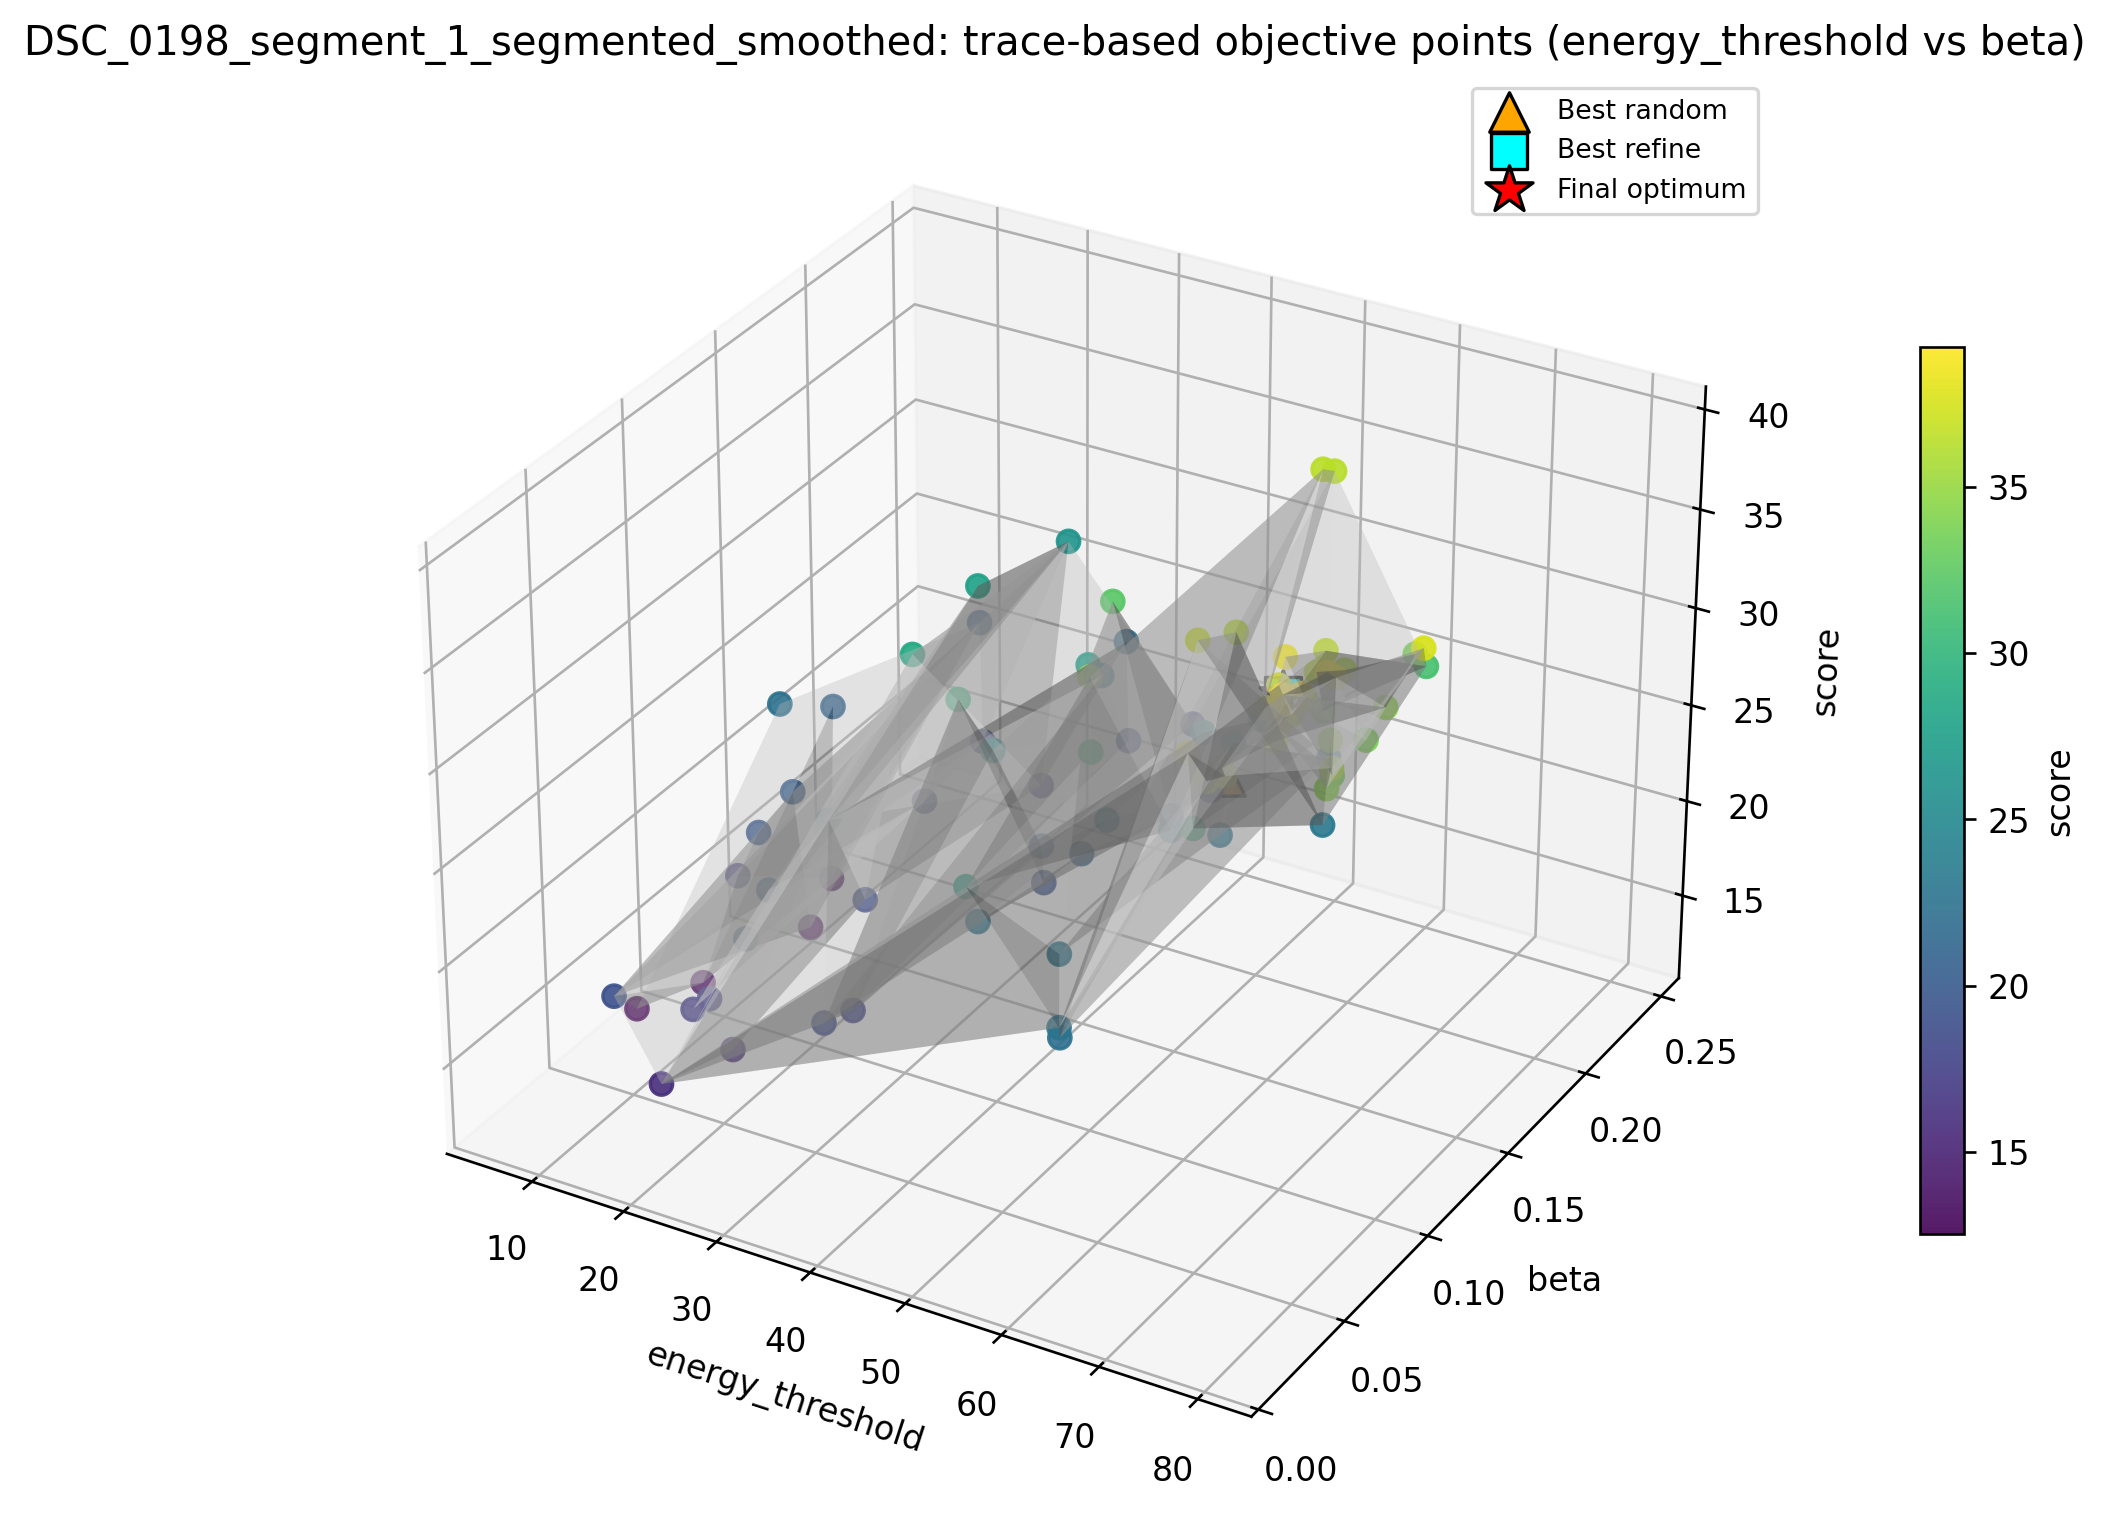
\includegraphics[width=\columnwidth]{surface_DSC_0198_segment_1_segmented_smoothed__surface_energy_threshold_vs_beta.png}
\caption{Trace-based projected objective surface ($T$ vs.\ $\beta$) for a representative \emph{high-score} leaf (DSC\_0198). All 112 evaluated candidates are shown as scatter points colored by score; the final optimum (red star), best random-phase point (orange triangle), and best refine-phase point (cyan square) are marked. A fitted triangulated surface is overlaid where sampling density permits.}
\label{fig:surface_high}
\end{figure}

\begin{figure}[!t]
\centering
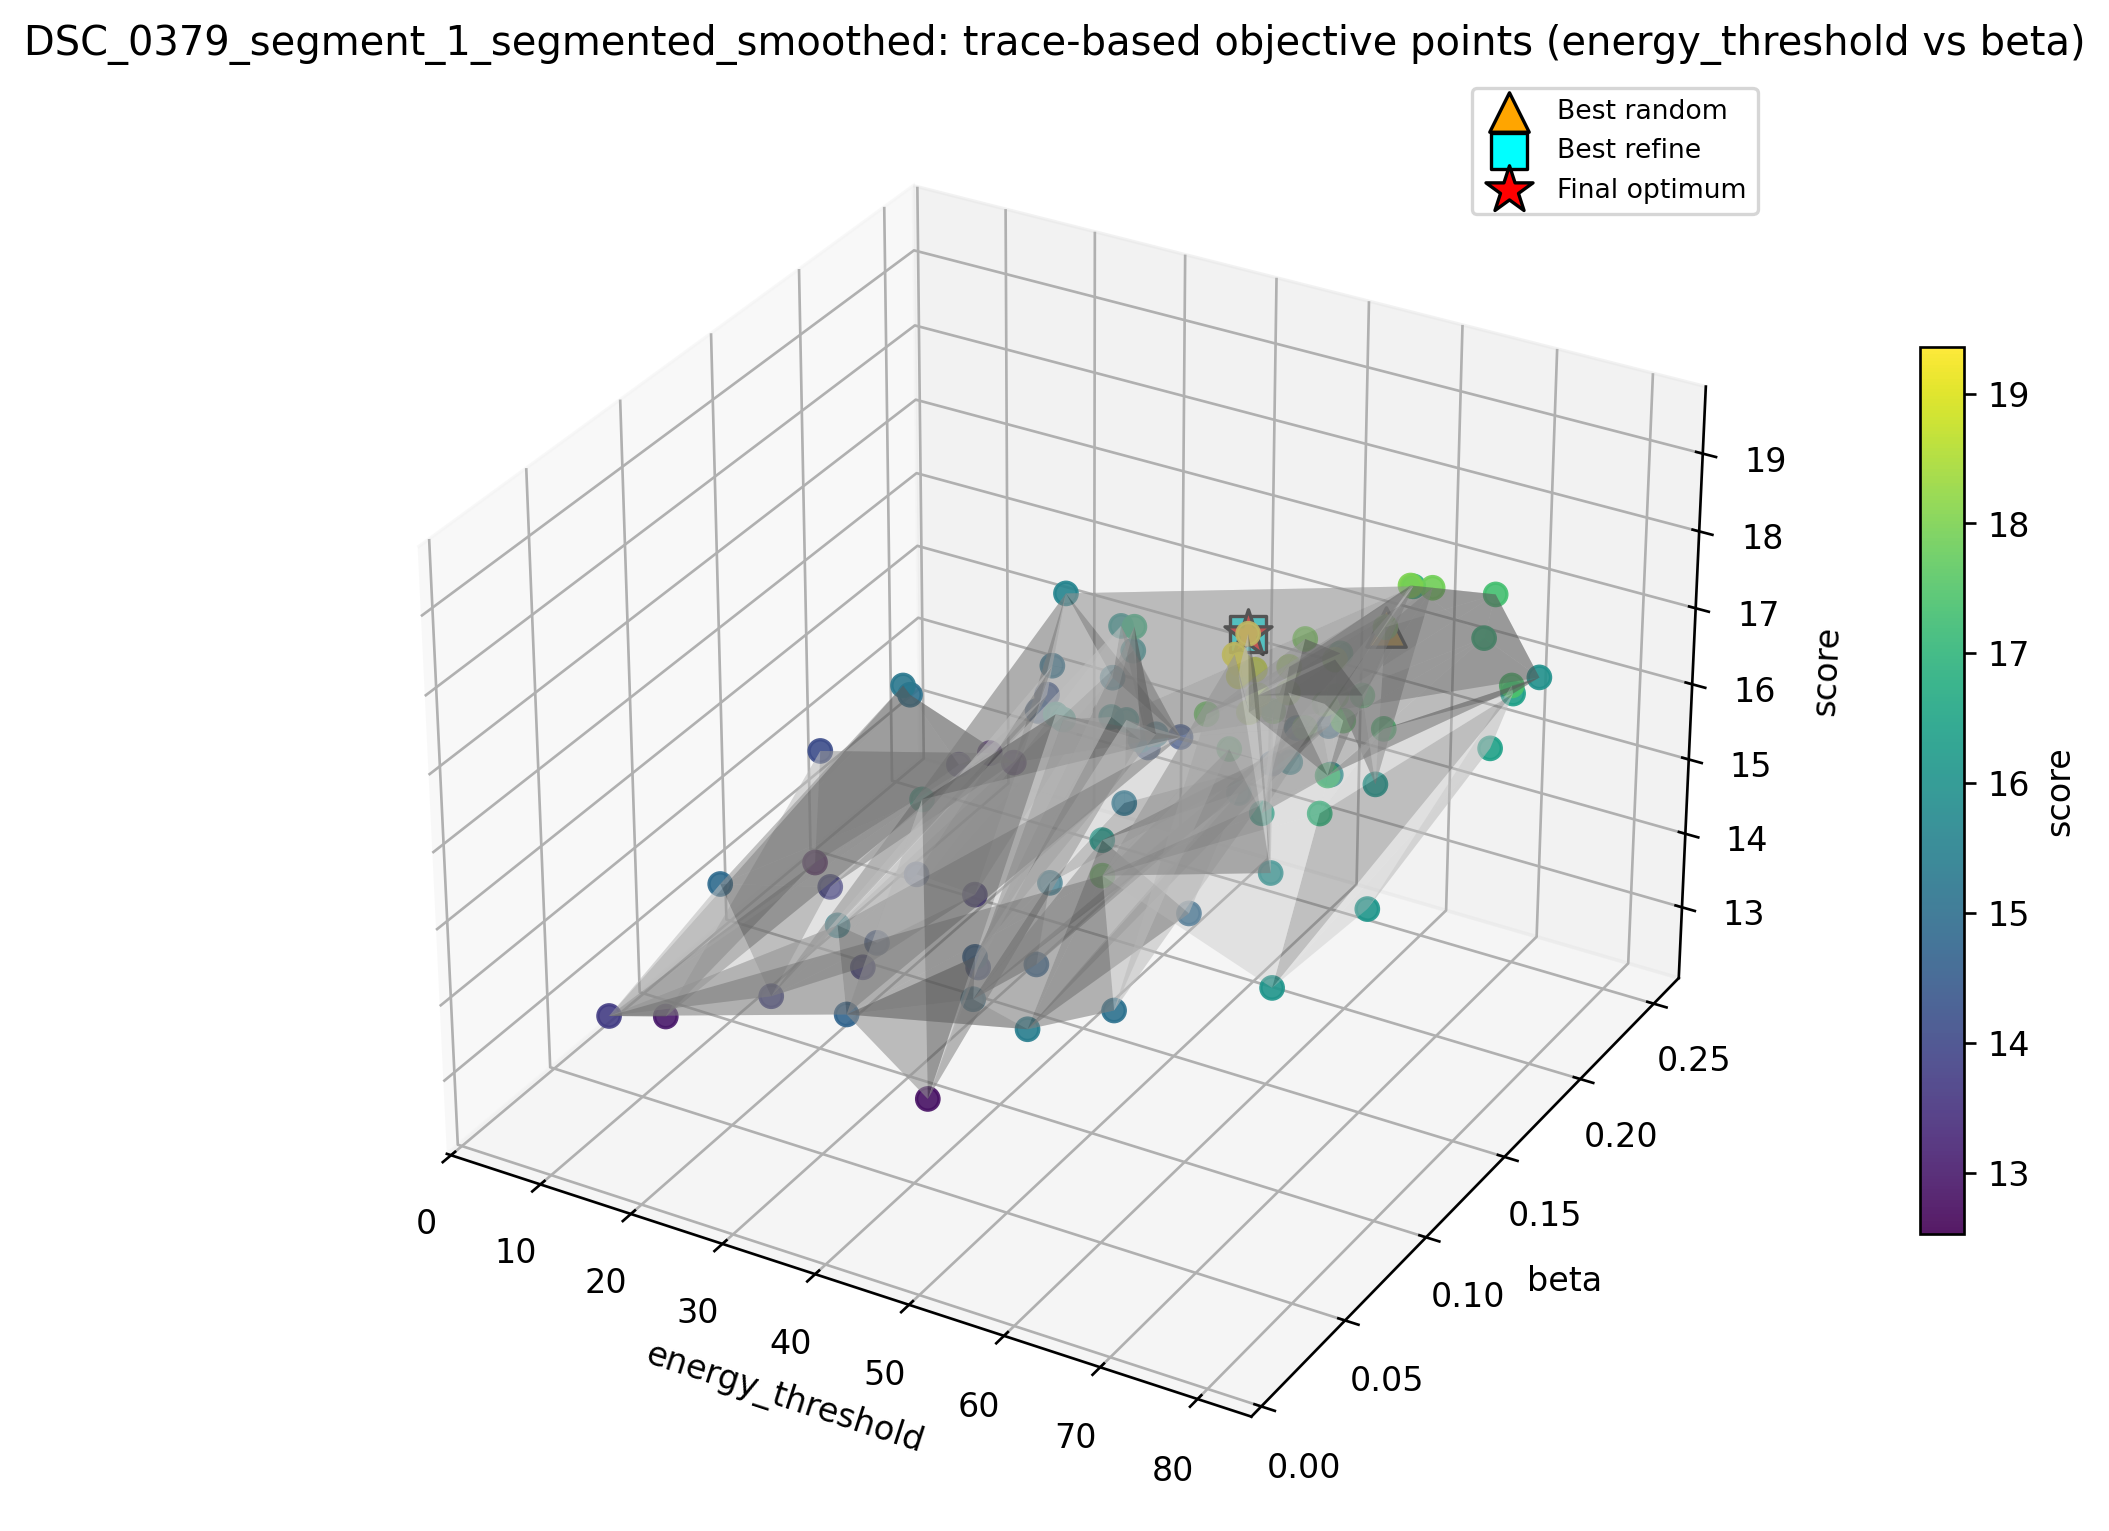
\includegraphics[width=\columnwidth]{surface_DSC_0379_segment_1_segmented_smoothed__surface_energy_threshold_vs_beta.png}
\caption{Trace-based projected objective surface ($T$ vs.\ $\beta$) for a representative \emph{median-score} leaf (DSC\_0379).}
\label{fig:surface_med}
\end{figure}

\begin{figure}[!t]
\centering
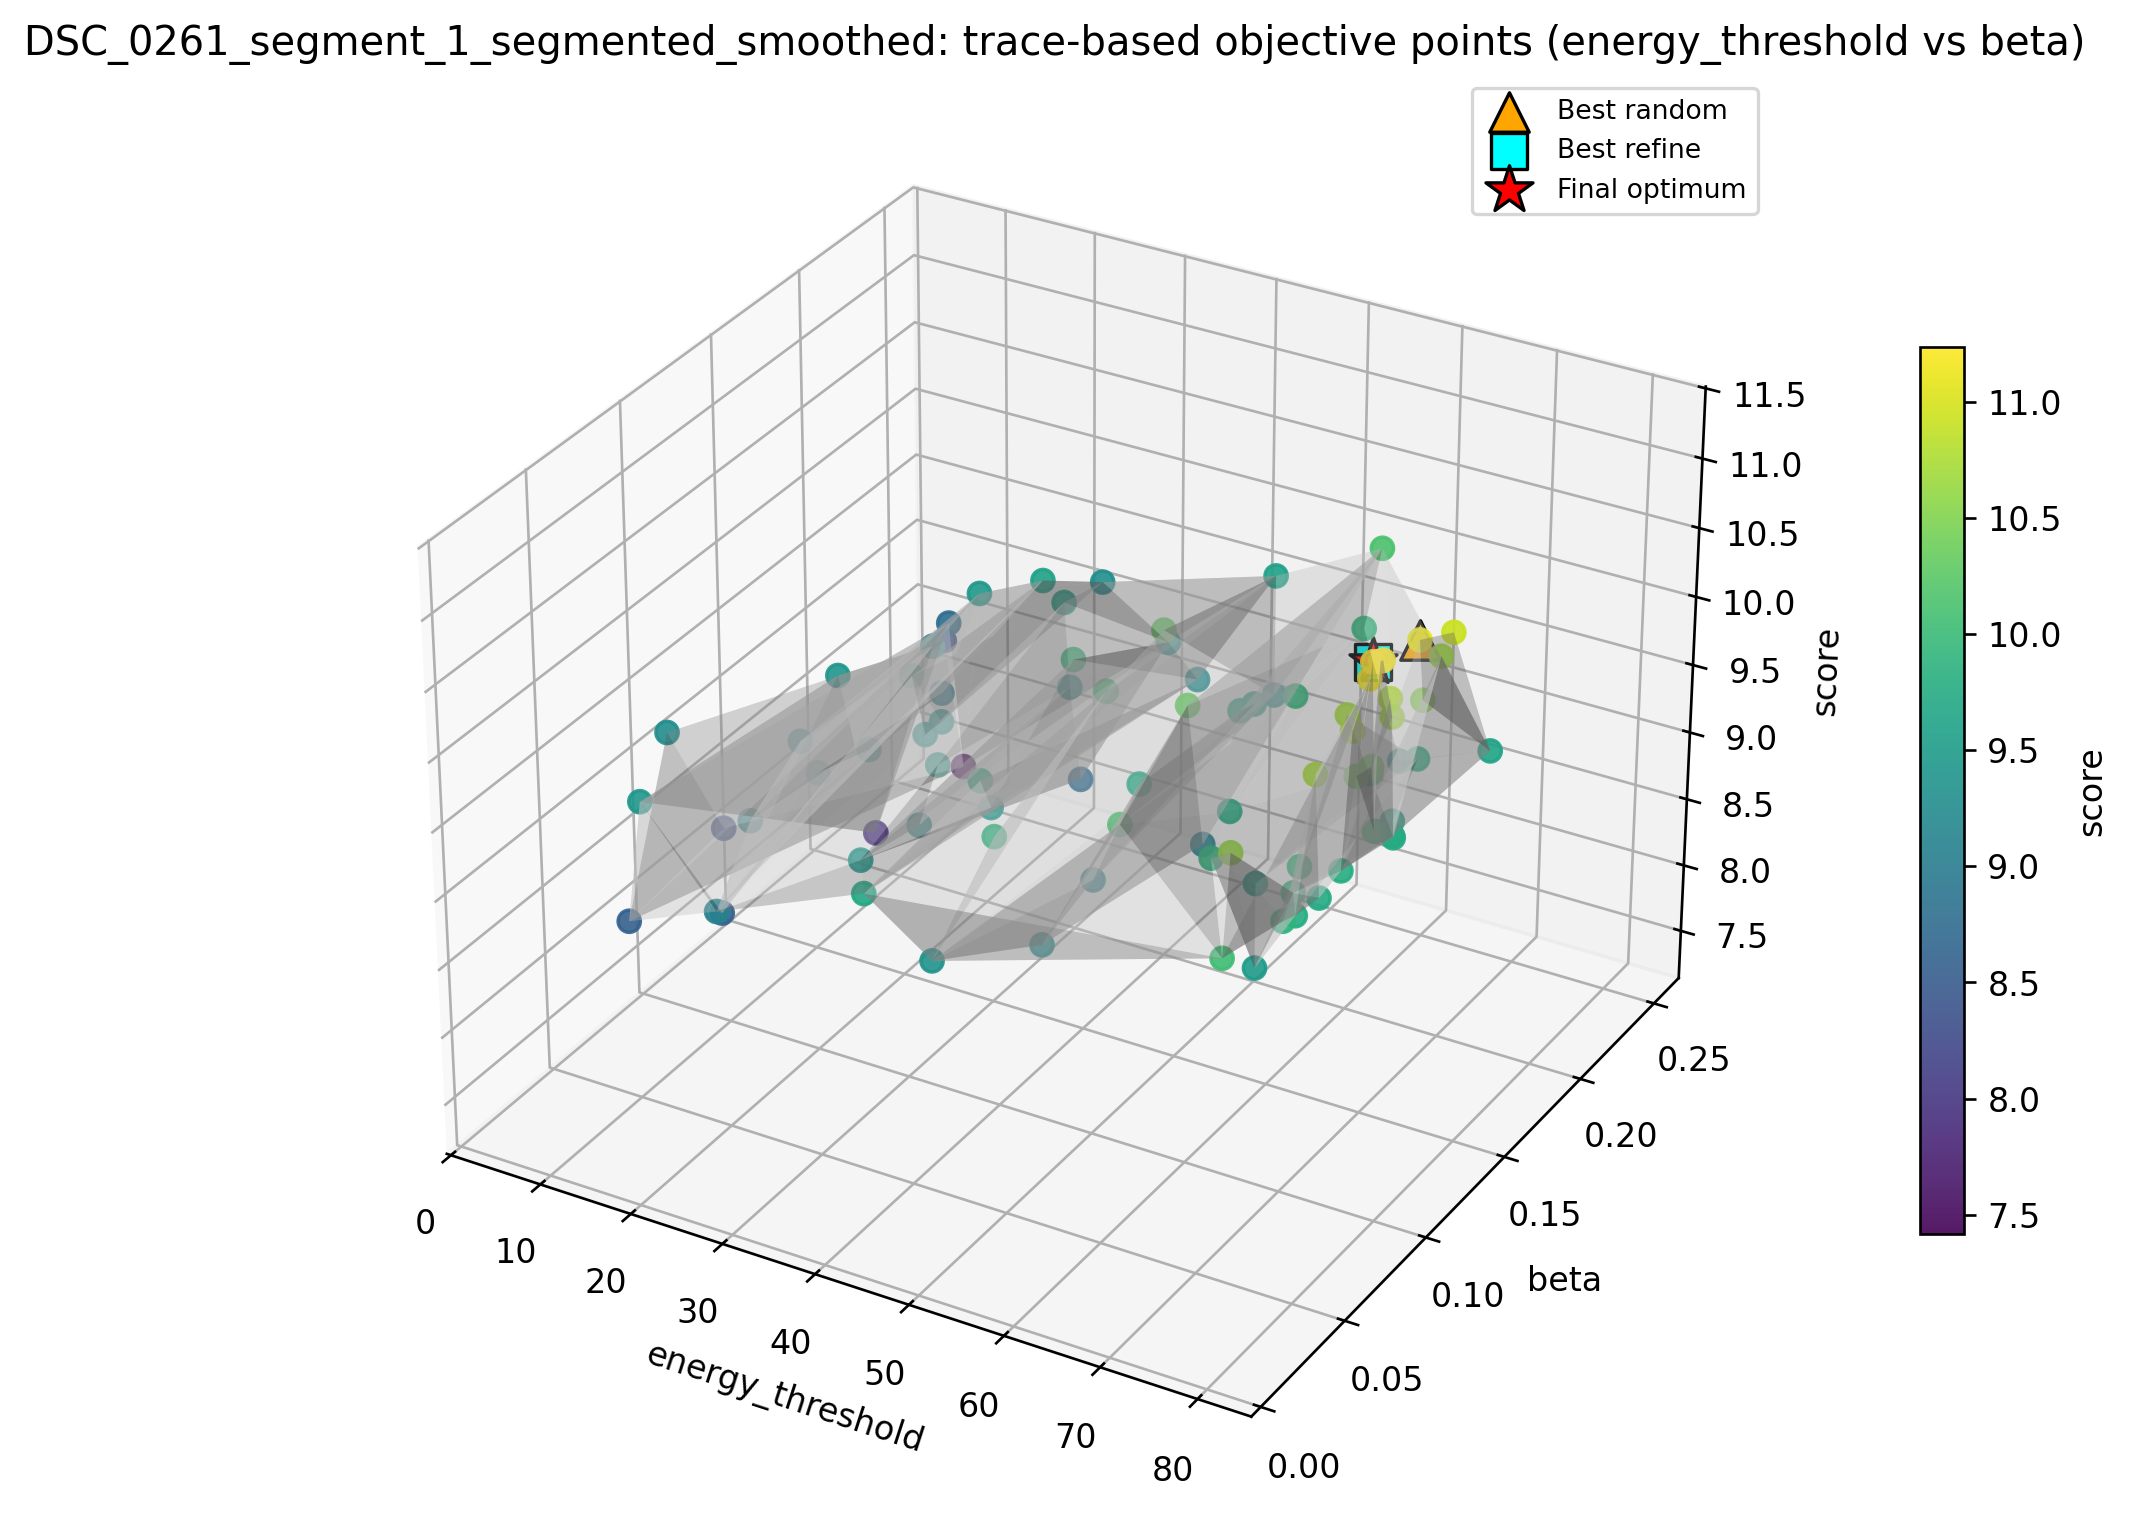
\includegraphics[width=\columnwidth]{surface_DSC_0261_segment_1_segmented_smoothed__surface_energy_threshold_vs_beta.png}
\caption{Trace-based projected objective surface ($T$ vs.\ $\beta$) for a representative \emph{low-score} leaf (DSC\_0261). The surface is flatter than for high-score leaves, consistent with a landscape that offers limited exploitable curvature.}
\label{fig:surface_low}
\end{figure}

\subsubsection{Optimization Trajectories}
Figure~\ref{fig:trajectory_high} shows the convergence of best-score-so-far for a high-score leaf, demonstrating the transition from random exploration (blue) to targeted refinement (orange). The refine phase achieves a distinct score improvement, confirming that local search around top random candidates is beneficial for morphologically complex leaves. For low-score leaves, the best-so-far curve plateaus early during random sampling, and the refine phase produces negligible gains.

\begin{figure}[!t]
\centering
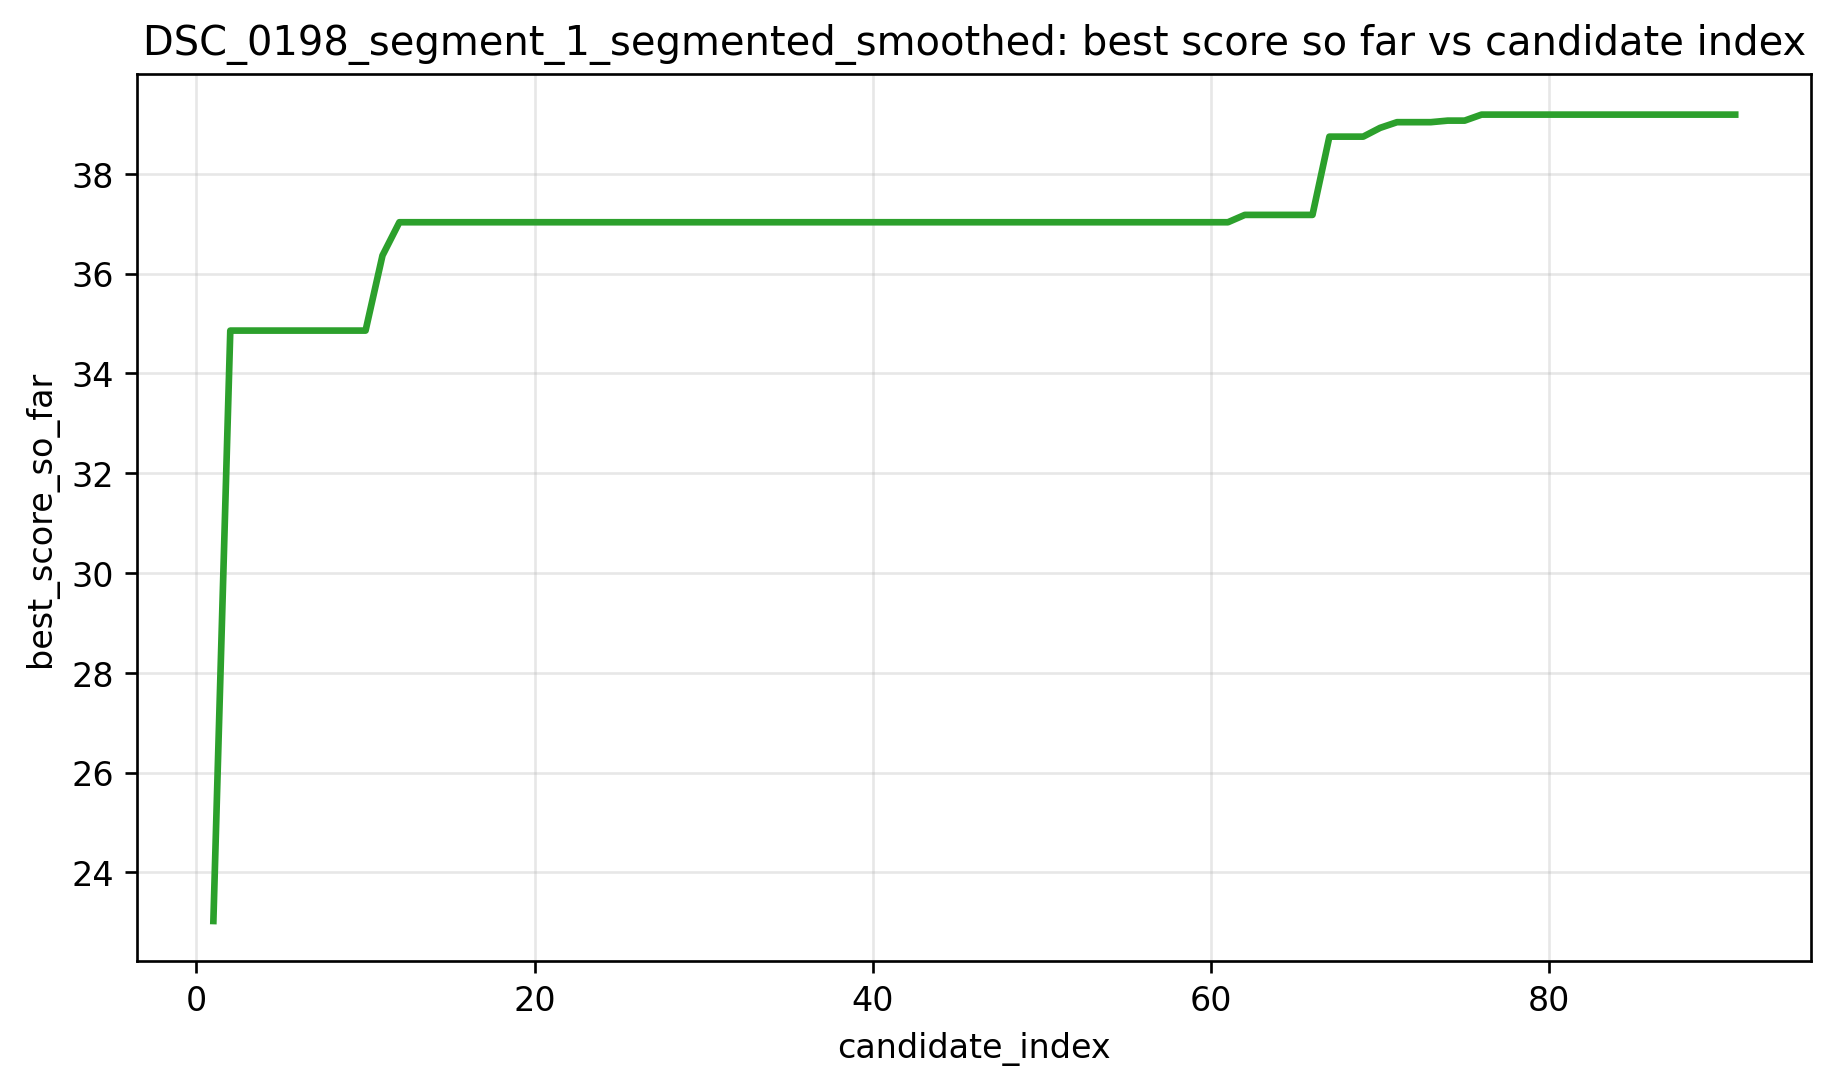
\includegraphics[width=\columnwidth]{traj_DSC_0198_segment_1_segmented_smoothed__trajectory_best_score_so_far.png}
\caption{Convergence trajectory: best score so far vs.\ candidate index for a high-score leaf (DSC\_0198). Random-phase candidates (blue region) establish initial optima; refine-phase candidates (orange region) improve upon them.}
\label{fig:trajectory_high}
\end{figure}

\subsubsection{Landscape Geometry Across Score Tiers}
Across the nine leaves, the dominant parameter pair (highest $R^2$ when regressing score on a two-parameter linear model) is consistently $T$--$\beta$, followed by $T$--$\mu$. This aligns with the physical interpretation: energy threshold controls which edges are detected, and balloon force controls how aggressively contours expand, making this pair the primary determinant of mask area and topology. A heuristic multi-basin analysis (based on spread of top-quartile candidates in normalized parameter space) finds hints of multiple basins in some high-score leaves, suggesting the landscape can support distinct good solutions corresponding to different segmentation strategies (e.g., many small lesions vs.\ fewer large coalesced regions).

% ==========================
\subsection{Parameter-Cloud Geometry and Manifold Structure}
\label{sec:param_geometry_results}
% ==========================
Complementing the score-landscape analysis above, we characterize the \emph{geometric organization} of the optimizer's solutions in the 7-dimensional parameter space (Section~\ref{sec:param_geometry_math}). Using 150 global--local parameter pairs from 15 leaves (75 interior, 75 boundary patches), we project parameter vectors via PCA and nonlinear embeddings.

\subsubsection{PCA Separation of Global and Local Optima}
Figure~\ref{fig:pca2d_global_local} shows the PCA 2D projection of all global (full-leaf) and local (patch-level) parameter vectors, colored by Dice improvement $\Delta D$. Two principal components capture 46.5\% of the total variance. Notably, PC1 separates the global and local clouds with a centroid shift magnitude of 1.616 standardized units, confirming that local re-optimization produces a \emph{systematic, directional} displacement in parameter space rather than random perturbation.

\begin{figure}[!t]
\centering
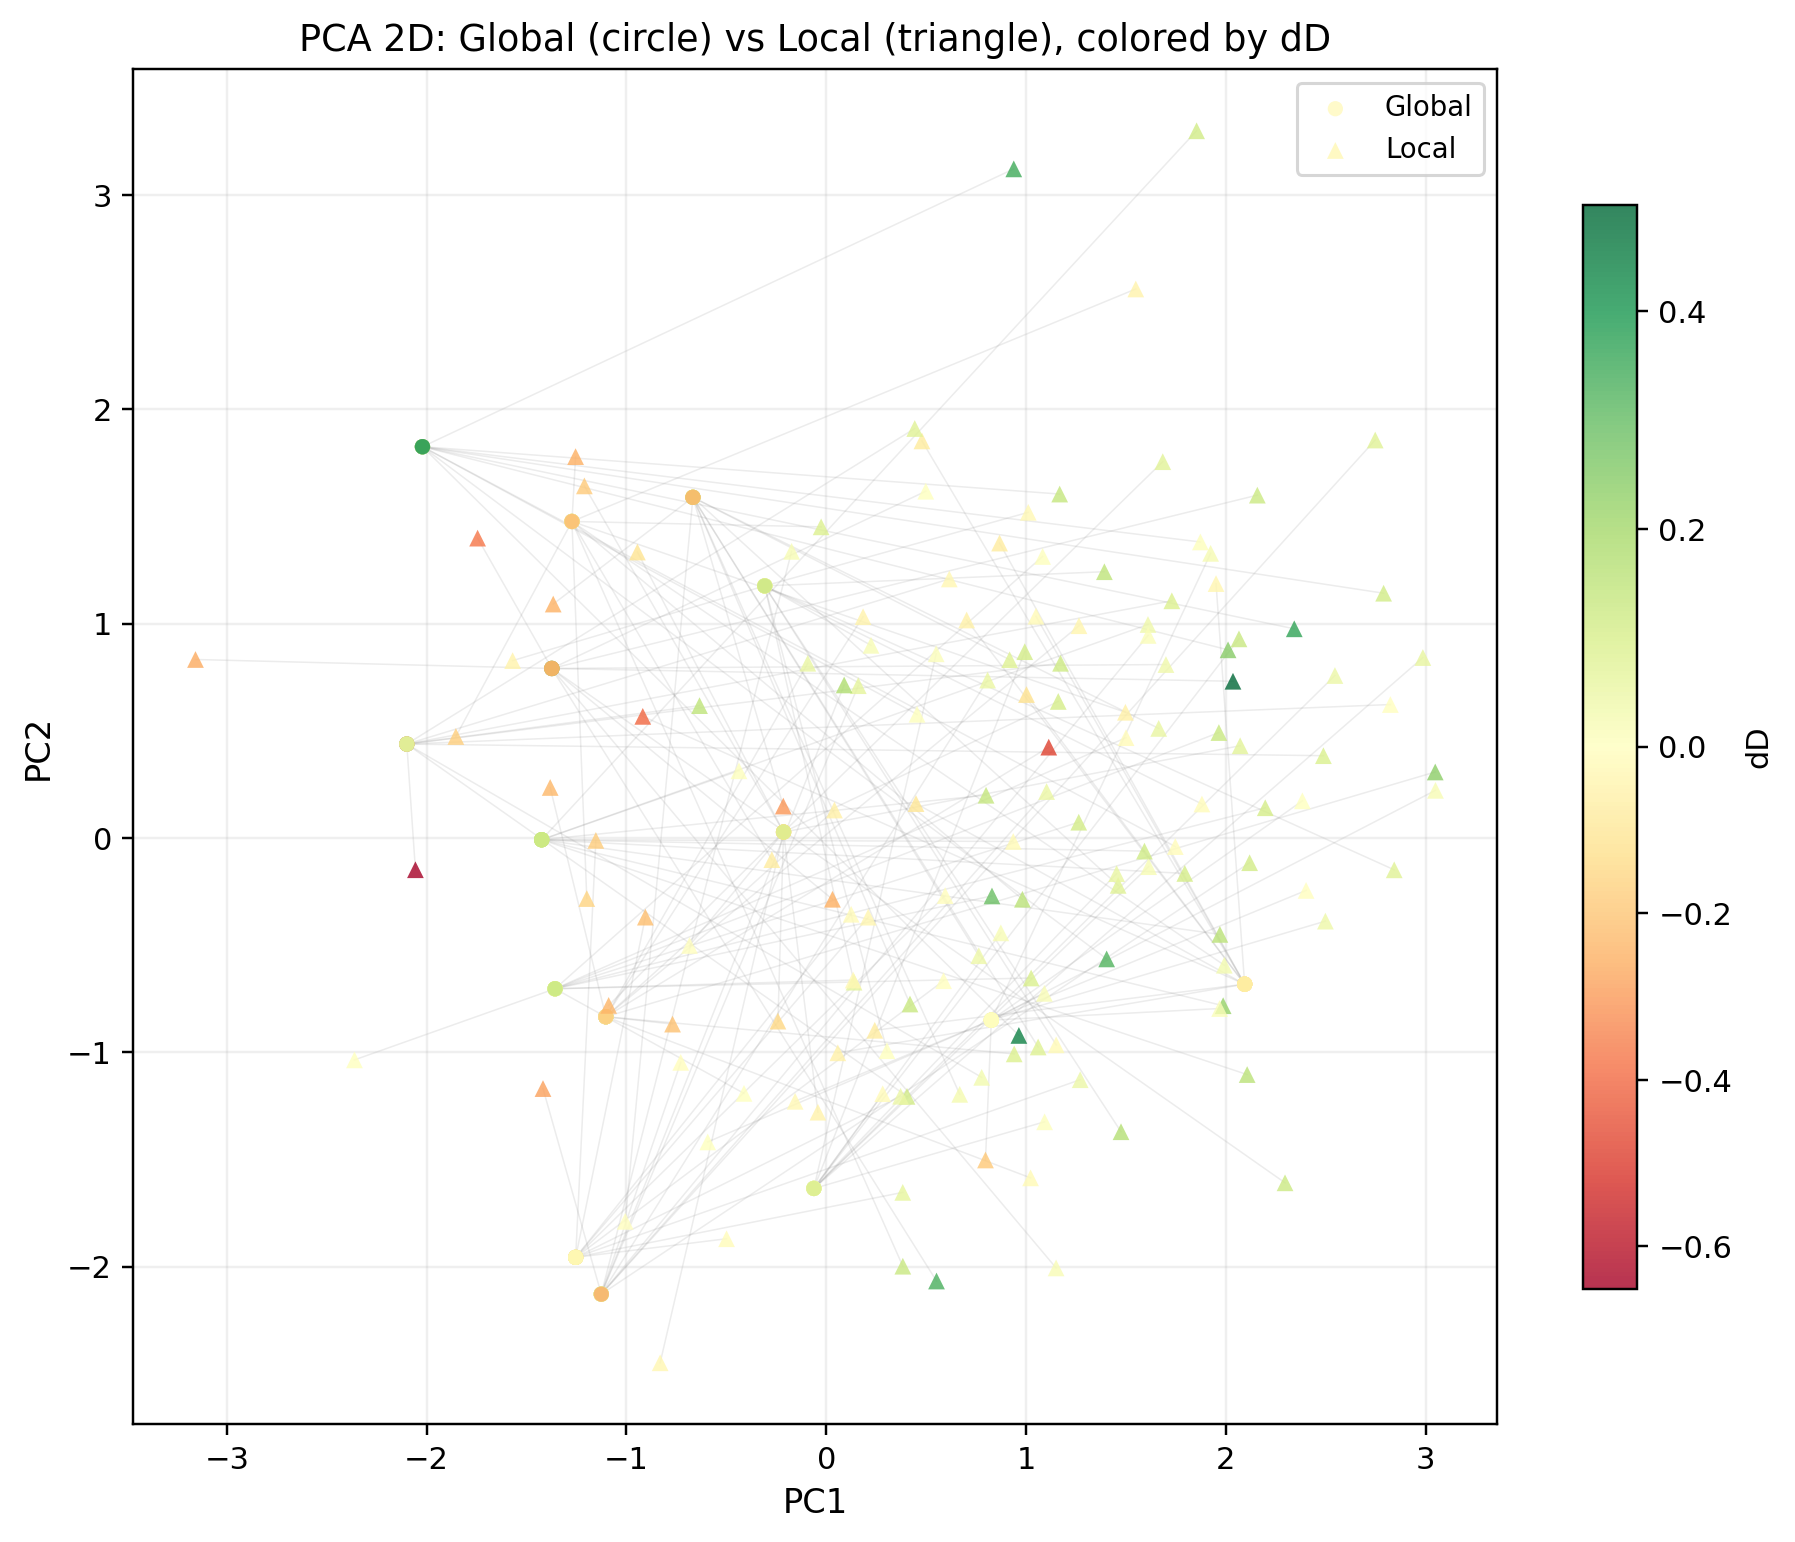
\includegraphics[width=\columnwidth]{pca2d_global_local_dD.png}
\caption{PCA 2D projection of global (circles) and local (triangles) parameter vectors from 150 patches. Points are colored by Dice improvement $\Delta D$. PC1 separates the two clouds, indicating a systematic directional shift from global to local optimization. The centroid shift magnitude is 1.616 standardized units.}
\label{fig:pca2d_global_local}
\end{figure}

\subsubsection{Mean Parameter Shift Profile}
Figure~\ref{fig:mean_delta} shows the mean parameter shift $\bar\delta$ across all patches. Energy threshold dominates, with $\mu$, diffusion rate, and $\gamma$ also contributing significant systematic shifts. This profile is consistent across interior and boundary patches, confirming that patch location does not determine the optimization trajectory---rather, the lesion content within the patch matters more.

\begin{figure}[!t]
\centering
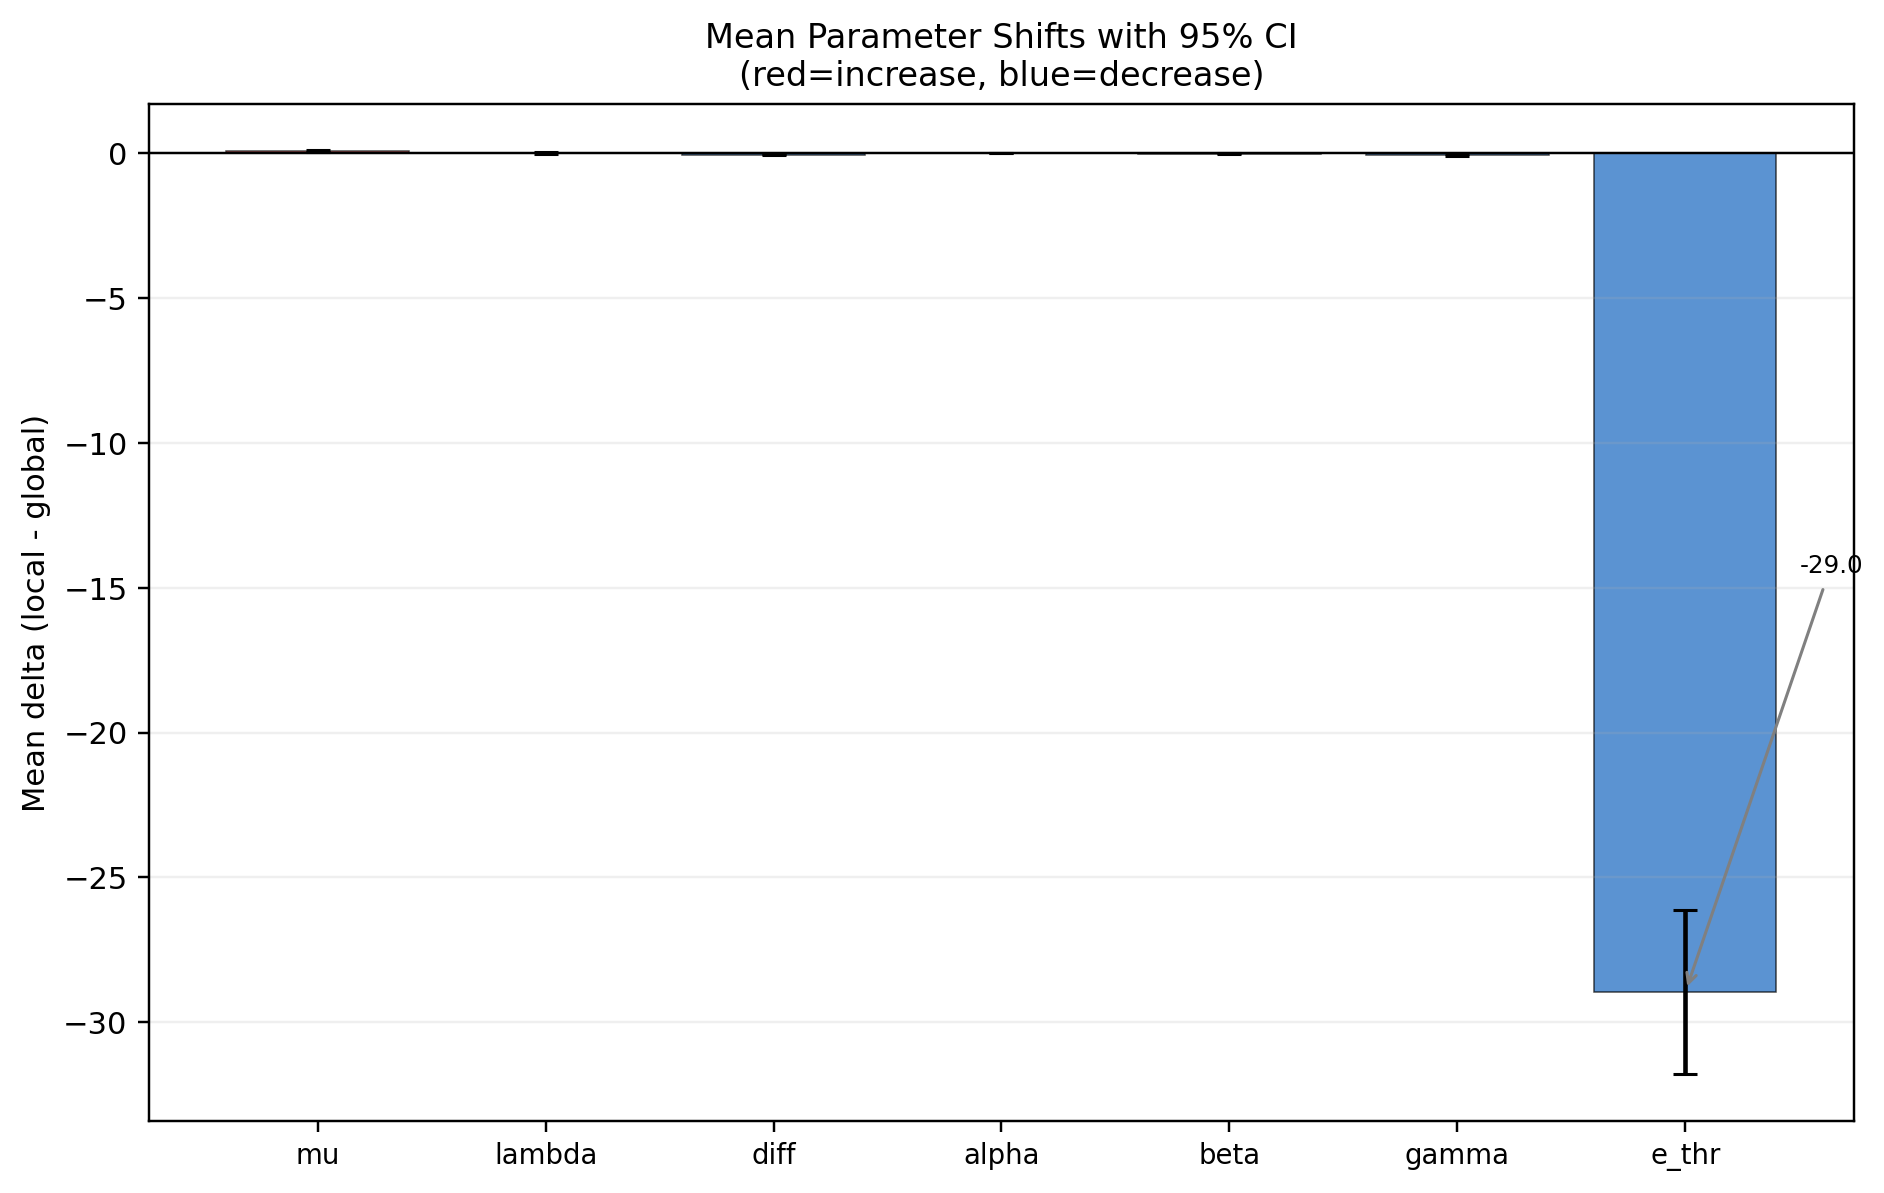
\includegraphics[width=\columnwidth]{mean_delta_parameters.png}
\caption{Mean parameter shift (global $\to$ local) across 150 patches. Energy threshold is the dominant shift parameter; $\mu$, diffusion rate, and $\gamma$ also show significant systematic displacements.}
\label{fig:mean_delta}
\end{figure}

\subsubsection{Solid 3D Geometry: Covariance Ellipsoids and Convex Hulls}
To visualize the volumetric organization of solution clouds, we fit 2-sigma covariance ellipsoids and convex hulls in PCA space (Figure~\ref{fig:cov_ellipsoids}). The global and local clouds form overlapping but displaced ellipsoids whose orientations are similar, suggesting that the optimization landscape has comparable curvature at both scales. The centroid shift arrow indicates the direction of systematic displacement. Patches where local optimization improved Dice ($\Delta D > +0.02$; $n{=}73$) and patches where it hurt ($\Delta D < -0.02$; $n{=}48$) show partial separation in PCA space, suggesting that the \emph{direction} of the parameter shift, not just its magnitude, encodes information about optimization success.

\begin{figure}[!t]
\centering
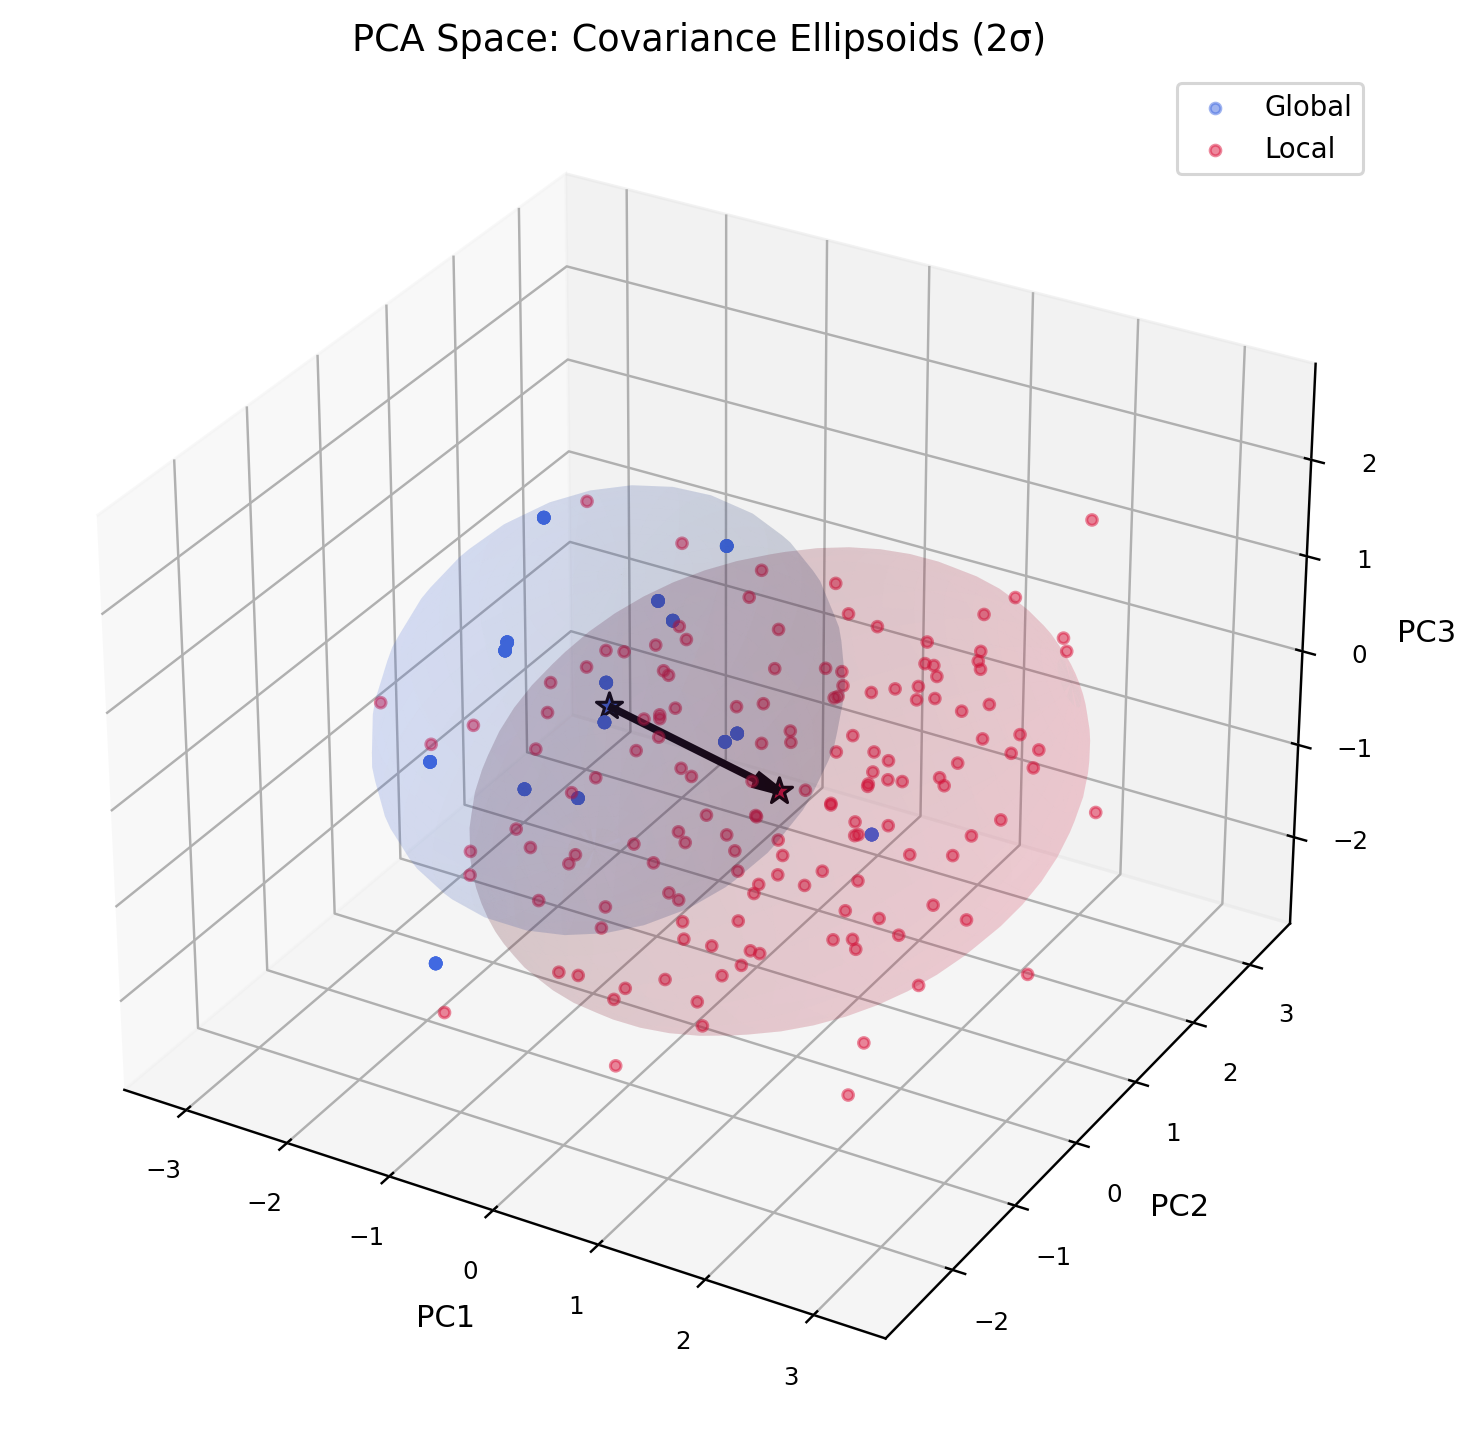
\includegraphics[width=\columnwidth]{pca3d_covariance_ellipsoids.png}
\caption{Covariance ellipsoids (2-sigma) for global (blue) and local (red) parameter clouds in PCA space. Star markers show centroids; black arrow indicates centroid shift direction. The ellipsoids overlap substantially but are systematically displaced, confirming structured parameter organization.}
\label{fig:cov_ellipsoids}
\end{figure}

\subsubsection{Neighbor Consistency and Predictive Structure}
A $k$-NN classification test on the delta-parameter cloud yields agreement of 0.534 for $\Delta D$ groups (vs.\ random baseline 0.33), indicating that nearby points in parameter-shift space tend to share the same improvement outcome. Patch type (interior vs.\ boundary) achieves only 0.488 (baseline 0.50), confirming that spatial location within the leaf does not predict the parameter-shift direction. These findings support the feasibility of an amortized parameter predictor that maps image features to optimized parameters, since the parameter manifold encodes exploitable structure.

% ==========================
\subsection{Qualitative Results and Failure Taxonomy}
% ==========================
Figure~\ref{fig:qual_grid} organizes qualitative results across the Dice spectrum, spanning five biologically meaningful lesion categories:
\begin{itemize}
    \item Small discrete necrotic spots (strong edges),
    \item Chlorotic halos (soft edges),
    \item Coalescing/merged lesions,
    \item Mixed inner/outer structure (necrotic core + halo ring),
    \item Leaf venation confounds and glare artifacts.
\end{itemize}

\begin{figure*}[t]
\centering
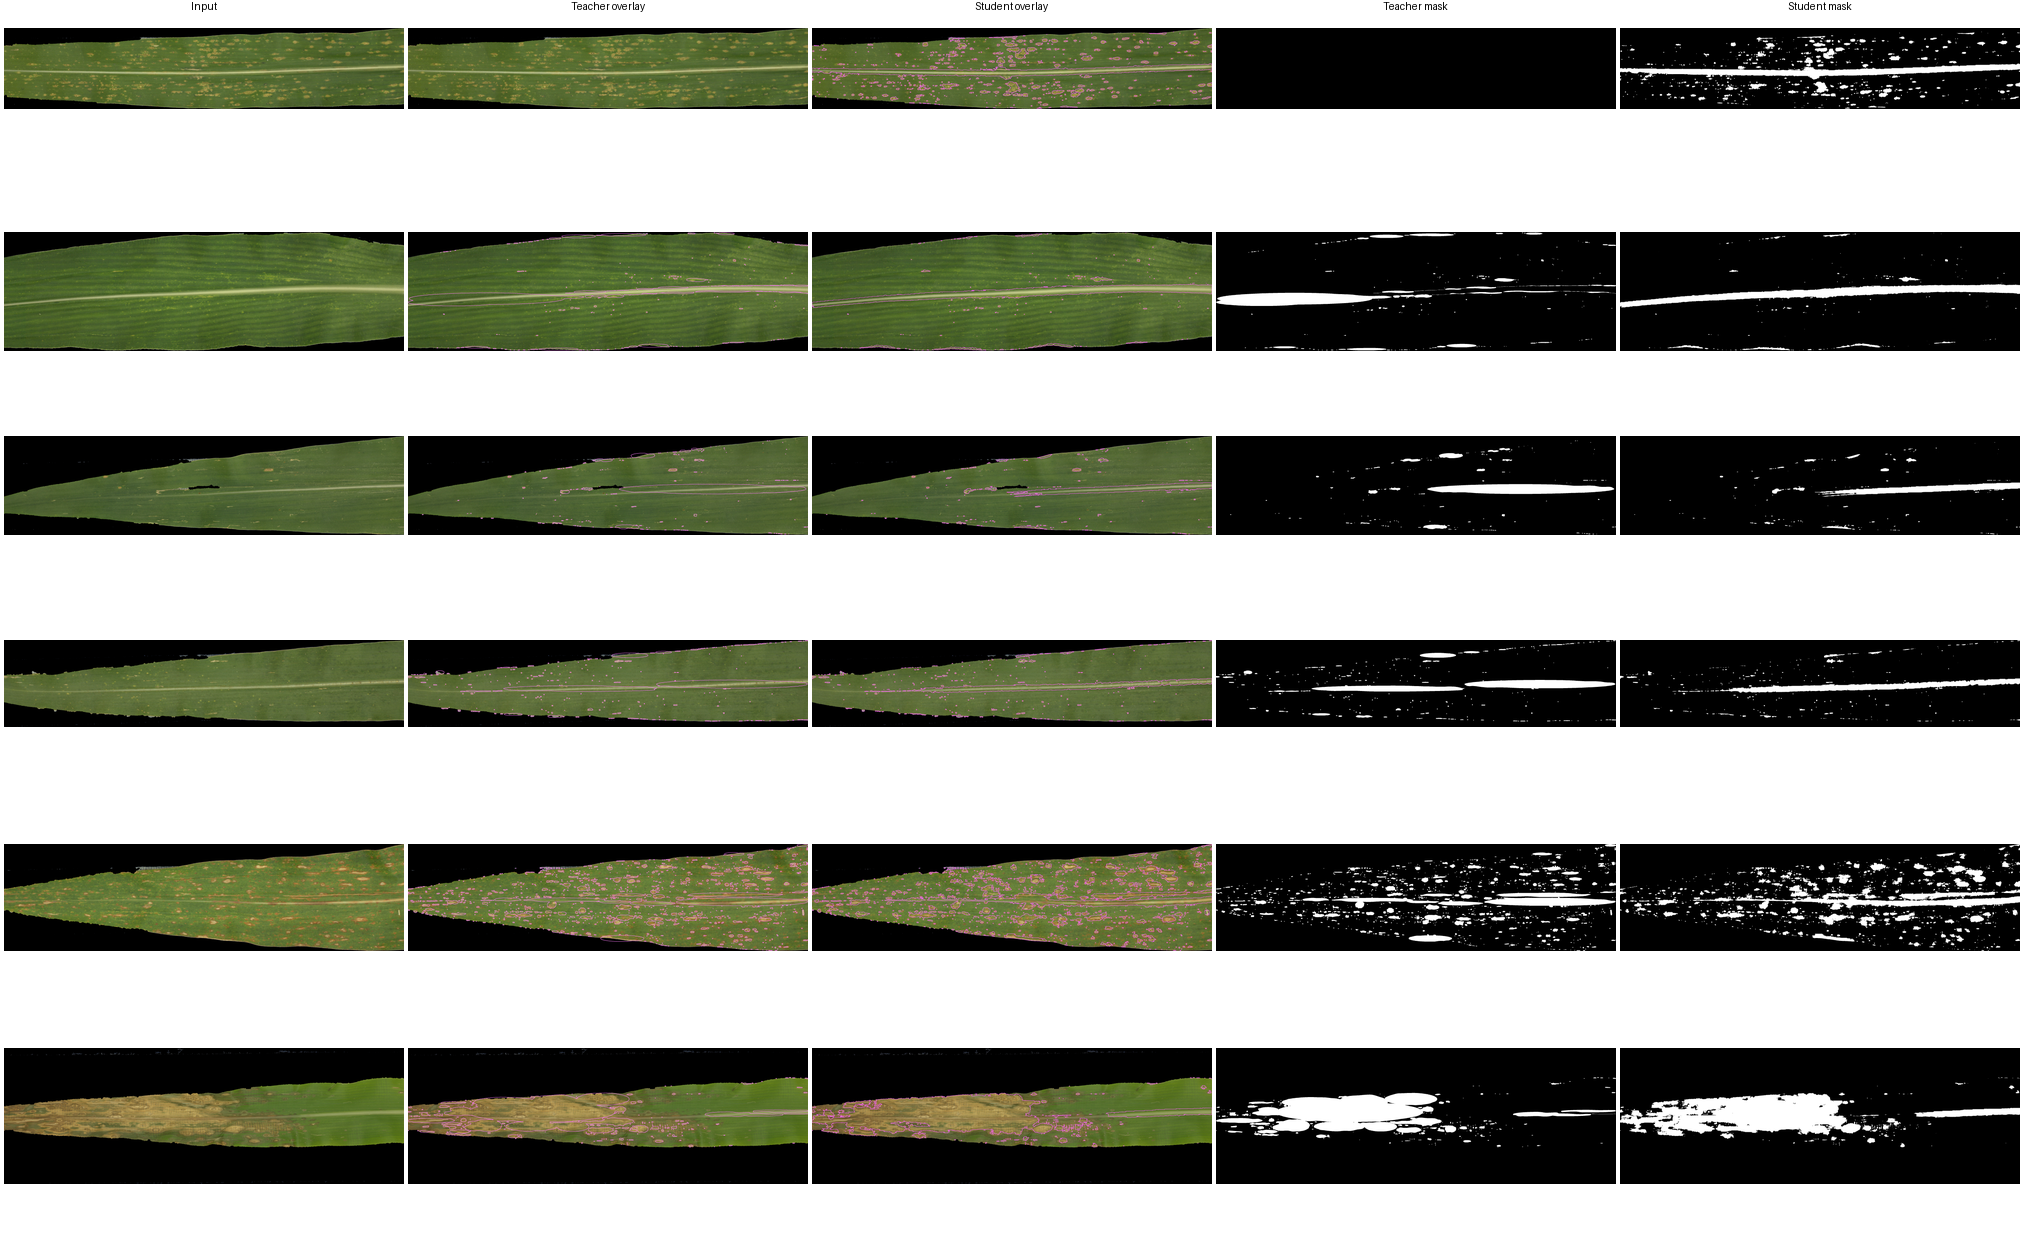
\includegraphics[width=\textwidth]{qual_grid_teacher_student.png}
\caption{Qualitative grid across the Dice spectrum (6 rows, sorted worst-to-best). Columns: Input leaf image, teacher (optimizer) overlay, student (UNet) overlay, teacher mask, student mask. Rows span Dice${\approx}0.0$ (teacher-empty case) to Dice${\approx}0.84$ (high agreement).}
\label{fig:qual_grid}
\end{figure*}

% ==========================
\section{Multi-Stage Inference for Nested/Inner Lesions}
\label{sec:multistage}
Broad lesions frequently contain inner oscillating or necrotic substructures that are biologically distinct from the outer chlorotic halo. We address this with a \textbf{two-stage nested inference strategy}:
\begin{enumerate}
    \item Stage-A (outer): run optimizer to obtain outer lesion regions $M_{\text{outer}}$.
    \item Stage-B (inner): restrict to $M_{\text{outer}}$ and re-run with a higher threshold $T'$ and slightly different snake rigidity to capture necrotic cores $M_{\text{inner}}$.
\end{enumerate}
This yields biologically meaningful \emph{nested masks} enabling traits such as:
\begin{equation}
\text{Necrosis ratio} = \frac{|M_{\text{inner}}|}{|M_{\text{outer}}|+\varepsilon},
\end{equation}
and enables better downstream phenotyping.

In practice, Stage-B may legitimately yield an empty $M_{\text{inner}}$ for lesions without a necrotic core; we treat these as biologically plausible ``no-inner cases in our teacher--student evaluation.

\begin{algorithm}
\caption{Two-Stage Nested Lesion Inference}
\label{alg:two_stage}
\begin{algorithmic}[1]
\REQUIRE Image $I$, search bounds $\Theta$
\STATE \textbf{Stage-A (Outer):} $\theta_A^\star \leftarrow \mathrm{Optimize}(I;\Theta)$
\STATE $M_{\text{outer}} \leftarrow \mathrm{RunPhysics}(I;\theta_A^\star)$ \COMMENT{green overlay}
\IF{$|M_{\text{outer}}| > 0$}
    \STATE \textbf{Stage-B (Inner):} Restrict search to pixels inside $M_{\text{outer}}$
    \STATE Increase energy threshold: $T' \leftarrow 1.3\,T_A^\star$
    \STATE $\theta_B^\star \leftarrow \mathrm{Optimize}(I \odot M_{\text{outer}};\Theta')$
    \STATE $M_{\text{inner}} \leftarrow \mathrm{RunPhysics}(I \odot M_{\text{outer}};\theta_B^\star)$ \COMMENT{magenta overlay}
\ELSE
    \STATE $M_{\text{inner}} \leftarrow \emptyset$
\ENDIF
\RETURN $M_{\text{outer}}, M_{\text{inner}}$
\end{algorithmic}
\end{algorithm}

In our visualization, Stage-A outer lesion boundaries are rendered as semi-transparent green overlays on the original 16-bit leaf image, while Stage-B inner necrotic cores are rendered in magenta, enabling visual separation of halo and necrotic regions in composite overlays.

% ==========================
\section{Discussion and Limitations}
% ==========================

\textbf{Global-parameter transfer under patchification.}
To assess whether per-leaf optimized physics parameters remain valid under patch-based processing, we performed a context-stability test using the optimal parameter set $\theta^\star$ obtained on each full-resolution leaf. Without re-optimizing on crops, we applied the same $\theta^\star$ in a \emph{finalize-only} run on local $512\times512$ patches and compared the resulting masks to the corresponding patch crops of the full-leaf teacher mask. Across sampled leaves and patches, we observed a median Dice agreement of $0.78$ (mean $0.72$), indicating that the per-leaf parameters transfer well to most local regions. However, agreement degraded for a subset of patches (10th percentile Dice $=0.34$), consistent with crop-boundary sensitivity of the PDE/snakes finalization (e.g., truncated context and boundary effects). In additional tests with reflect-padding around patches (not shown), this low-tail behavior reduced, further supporting a boundary-effect interpretation. This observation motivates our hybrid design: we execute the physics-based teacher on full leaves to generate pseudo-labels with minimal crop artifacts, and use the patch-based student network for efficient localized inference and stitching at full resolution.

\textbf{Patch-level morphology transfer: area and lesion-count fidelity.}
Beyond overlap metrics, we evaluated whether morphological quantities relevant to downstream phenotyping---specifically lesion area fraction and lesion count---are preserved when per-leaf parameters are transferred to patches.
Using the same 150 patches from 15 leaves (75 interior, 75 boundary), we ran the full finalize pipeline in forward-pass mode with the globally optimized $\theta^\star$ (``global'') and the locally re-optimized $\theta_{\mathrm{local}}^\star$ (``local''), and compared the resulting area fraction and connected-component count against the teacher mask.
Table~\ref{tab:patch_morph_transfer} summarizes the results.
Both parameter sets severely underestimate lesion area (global: $0.026$ vs.\ teacher $0.169$), suggesting that the two-stage inner-mask definition discards peripheral necrotic tissue that the teacher retains at full resolution.
Local re-optimization reduces mean absolute count error by 35\% ($19.1 \to 12.4$), with larger improvements on interior patches ($27.6 \to 18.6$), indicating that per-patch tuning recovers some lesion fragments lost to context truncation.
Overlap metrics (Dice, IoU) show only modest changes ($+0.013$ mean $\Delta$Dice), confirming that morphological fidelity and pixel-overlap can diverge and should be reported jointly in phenotyping applications~\citep{ronneberger2015u}.
This distinction is especially important in high-throughput phenotyping workflows where downstream trait extraction---lesion counts, area distributions, and necrotic ratios---constitutes the primary scientific output~\citep{gehan2017high,plantcv2025}; a segmentation with high Dice but biased morphological statistics can mislead quantitative trait analysis.

\begin{table}[t]
\centering
\caption{Patch-level morphology transfer: mean metrics across 150 patches (75 interior, 75 boundary). Area fraction is lesion area divided by valid pixels; count is connected components $\geq 16$\,px.}
\label{tab:patch_morph_transfer}
\setlength{\tabcolsep}{4pt}
\begin{tabular}{l c c c}
\hline
Metric & All & Interior & Boundary \\
\hline
Dice (global, teacher)       & 0.430 & 0.344 & 0.516 \\
Dice (local, teacher)        & 0.443 & 0.381 & 0.505 \\
$\Delta$Dice (local$-$global)& $+$0.013 & $+$0.037 & $-$0.011 \\
\hline
Teacher area frac            & 0.169 & 0.198 & 0.141 \\
Global area frac             & 0.026 & 0.026 & 0.026 \\
Local area frac              & 0.028 & 0.035 & 0.021 \\
$|$area frac err$|$ (global) & 0.143 & 0.171 & 0.115 \\
$|$area frac err$|$ (local)  & 0.141 & 0.163 & 0.120 \\
\hline
Teacher count                & 23.9 & 34.0 & 13.7 \\
Global count                 & 39.4 & 56.8 & 22.1 \\
Local count                  & 29.7 & 46.7 & 12.6 \\
$|$count err$|$ (global)     & 19.1 & 27.6 & 10.7 \\
$|$count err$|$ (local)      & 12.4 & 18.6 & 6.3 \\
\hline
\end{tabular}
\end{table}

\begin{figure}[t]
\centering
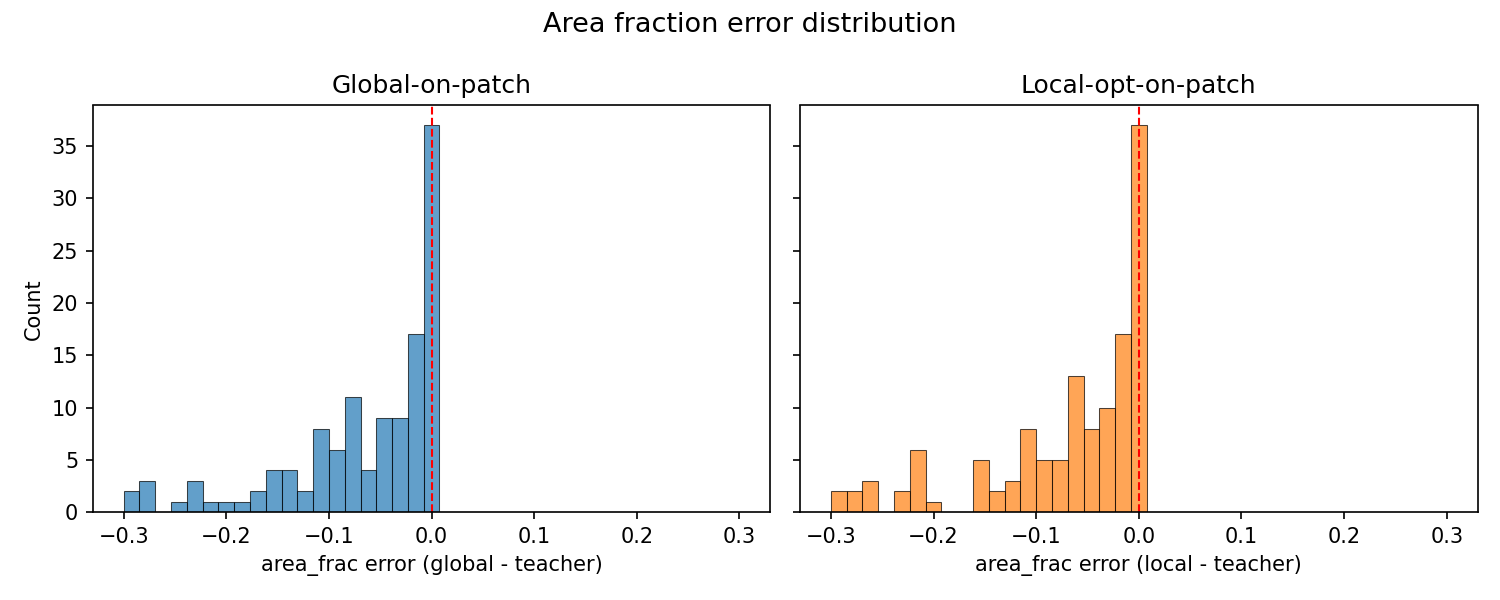
\includegraphics[width=\columnwidth]{hist_area_frac_error.png}
\caption{Distribution of signed area-fraction error (predicted $-$ teacher) for global and local parameter sets across 150 patches. Both distributions are left-skewed, reflecting systematic underestimation of lesion area under patchification.}
\label{fig:patch_area_err_hist}
\end{figure}

\begin{figure}[t]
\centering
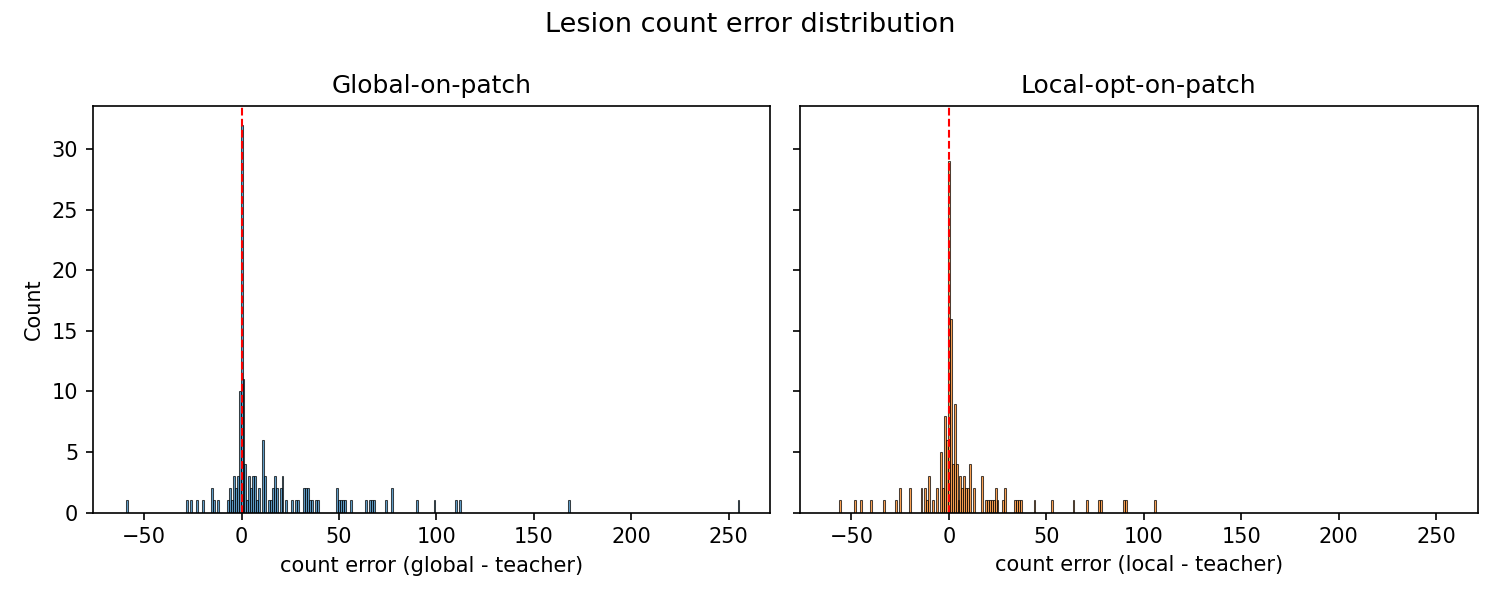
\includegraphics[width=\columnwidth]{hist_count_error.png}
\caption{Distribution of signed lesion-count error (predicted $-$ teacher). Local re-optimization shifts the distribution closer to zero, reducing mean $|$count error$|$ by 35\%.}
\label{fig:patch_count_err_hist}
\end{figure}

\begin{figure}[t]
\centering
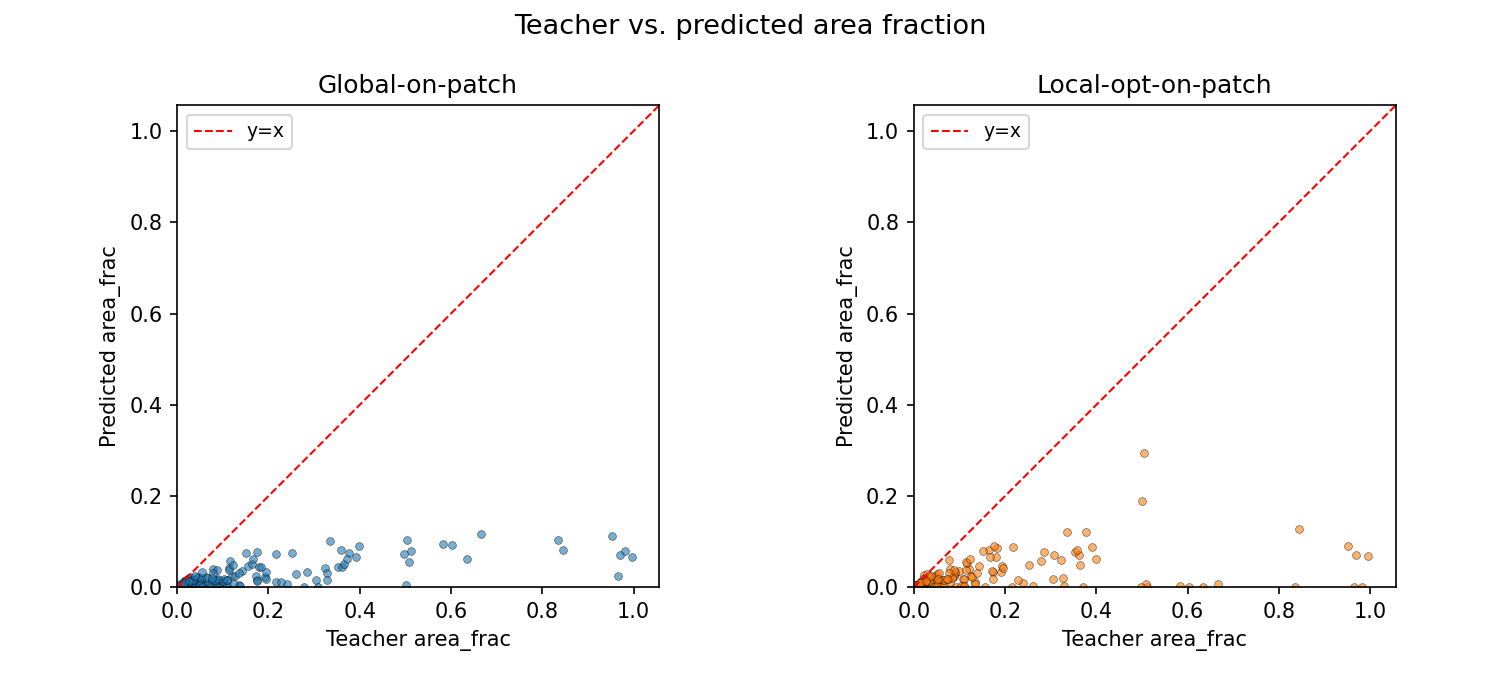
\includegraphics[width=\columnwidth]{scatter_teacher_vs_pred_area_frac.png}
\caption{Teacher vs.\ predicted lesion area fraction. Points below the diagonal indicate underestimation; both global and local predictions cluster well below the identity line, consistent with context-dependent area loss under patchification.}
\label{fig:patch_area_scatter}
\end{figure}

\textbf{Objective landscape geometry and search efficiency.}
The trace-based surface analysis (Section~\ref{sec:trace_analysis}) reveals that the objective landscape varies systematically with phenotypic difficulty. High-score leaves (morphologically favorable for segmentation) present landscapes with appreciable local curvature in the $T$--$\beta$ plane, rewarding the refine phase with measurable score gains. Low-score leaves (morphologically challenging) tend toward flatter landscapes where random exploration already approaches the optimum, and local refinement contributes minimally. This dichotomy has practical implications: for images with favorable phenotypes, budgeting more refinement steps could improve results; for difficult images, the search budget is better spent on broader exploration or alternative scoring strategies. The dominance of the $T$--$\beta$ parameter pair in explaining score variance confirms the central role of edge detection sensitivity and contour expansion in determining segmentation quality, consistent with the physics of the underlying PDE/snake pipeline.

These findings also relate to broader work on black-box optimization landscape analysis~\citep{hansen2001cma,jones1998ego}: the observation that some images present essentially ``trivial'' (flat) landscapes while others present rich, multimodal surfaces suggests that adaptive budget allocation---spending more evaluations where the landscape rewards exploration---could improve overall pipeline efficiency.

\textbf{Parameter-manifold structure and amortized prediction.}
The PCA and $k$-NN analysis of parameter clouds (Section~\ref{sec:param_geometry_results}) reveals that the optimizer's solutions are not scattered randomly in $\R^7$ but exhibit structured, optimizer-derived parameter organization: two PCs capture 46.5\% of variance, and the direction of the parameter shift from global to local optimization partially predicts whether local re-optimization helps ($k$-NN agreement 0.534 vs.\ random 0.33). We emphasize that this is a statement about the geometry of the optimizer's output space, not a claim that the method learns the governing physics from images. The practical implication is that amortized parameter prediction is feasible: a lightweight network mapping image features to $\theta^\star$ has an exploitable, structured target space rather than an arbitrary high-dimensional target. The dominance of energy threshold in the shift profile is consistent with the physics of the PDE pipeline---threshold determines which edges participate in contour initialization---but the primary observation is operational: local re-optimization chiefly adjusts edge-detection sensitivity to match patch contrast. Machine learning approaches to hyperparameter transfer and landscape characterization~\citep{yu2020hyperparam,singh2016machine} could further exploit this manifold structure for efficient multi-image optimization.

Our approach provides annotation-free segmentation but has other limitations:
\begin{itemize}
    \item Objective mismatch: Eq.~\eqref{eq:objective} is a proxy and can prefer wrong masks (e.g., veins) if color calibration fails.
    \item Runtime: per-image optimization is slower than feed-forward networks; practical use motivates distillation \citep{hinton2015distilling}.
    \item Domain shift: changes in lighting/camera or cultivars may change Lab separability, requiring re-tuning objective weights.
    \item Teacher noise: pseudo-labels derived from the inner-mask definition can be empty on some images even when outer lesions are present, creating teacher--student disagreements. We therefore report both overall agreement and conditional metrics on teacher-nonempty images. Adjudicating these cases with a small manually annotated subset would further clarify whether disagreements reflect optimizer false negatives or genuine semantic mismatches, and is reserved as a natural extension of this work.
\end{itemize}
\paragraph{Reproducibility and data availability.}
All optimizer code, ablation scripts, configuration files, and the 30-image ablation manifest are released under an open-source license. The stochastic search uses a fixed seed (1337 for ablations, 42 for subset selection), and all per-image parameter summaries (CSV) are included so that results can be reproduced without re-running the optimizer. The 174-image leaf dataset originates from controlled greenhouse experiments; leaf images were acquired under standardized lighting and are stored as lossless 16-bit TIFFs. We do not use human subjects data, and all plant material was grown under institutional biosafety protocols. We will release the annotation subset manifest ($N{=}60$) and the param-morphology metrics table alongside the code repository upon publication.

% ==========================
\section{Conclusion}
% ==========================
We have presented a fully automated pipeline for unsupervised lesion segmentation using Navier/elastic energy maps, multi-contour snakes, and per-image gradient-free stochastic optimization. By replacing manual parameter tuning with a robust objective and search strategy, we enable physics-based segmentation to adapt to heterogeneous lesion phenotypes in high-bit-depth imagery. Trace-based objective-surface analysis reveals that the difficulty of optimization correlates with phenotypic complexity: morphologically favorable images present sharp, exploitable landscapes, while challenging images yield flatter surfaces where random sampling suffices. Analysis of the optimizer's solution geometry shows that per-image parameters occupy a structured, low-dimensional manifold whose shift direction partially predicts optimization success, supporting the feasibility of amortized parameter prediction for future work. The output masks and per-image parameters naturally support downstream phenotyping and facilitate training of compact student models for fast inference.

\appendix
\section{Additional Optimizer Diagnostics}
To complement the main results, we report additional summary statistics of the stochastic optimizer, including output morphology distributions (mask area and component counts) and the empirical distributions of optimized parameters. Such diagnostics are useful in high-throughput phenotyping pipelines where downstream traits (e.g., lesion counts and area distributions) are primary outputs, and not fully characterized by overlap metrics alone (cf.\ PlantCV-style phenotyping workflows and trait extraction~\citep{plantcv2025}).

\begin{figure*}[!t]
\centering
\begin{minipage}[b]{0.49\textwidth}
\centering
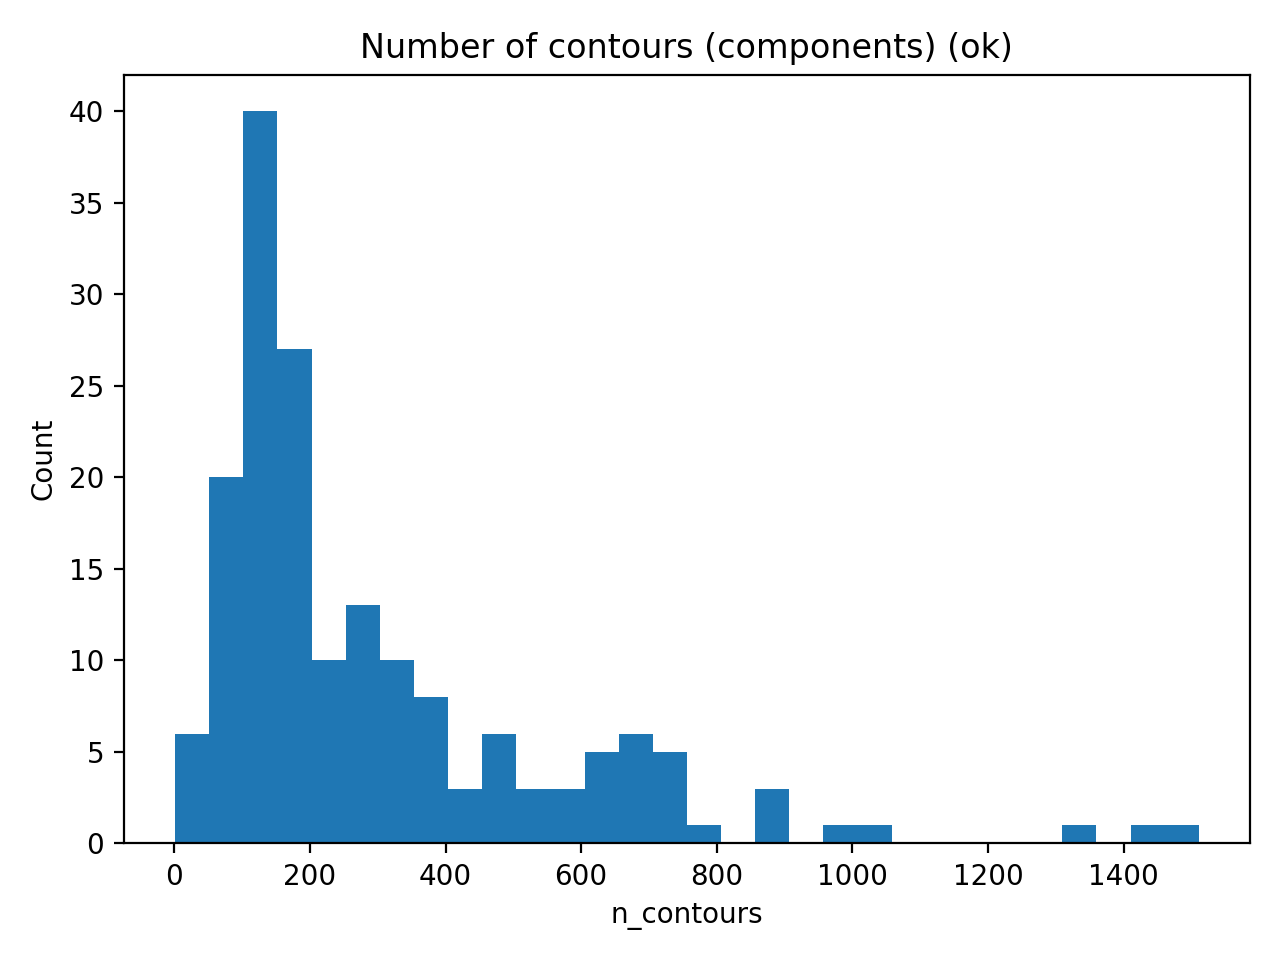
\includegraphics[width=\linewidth]{n_contours_hist.png}
\caption*{(a) Connected-component count ($n_c$) distribution.}
\end{minipage}\hfill
\begin{minipage}[b]{0.49\textwidth}
\centering
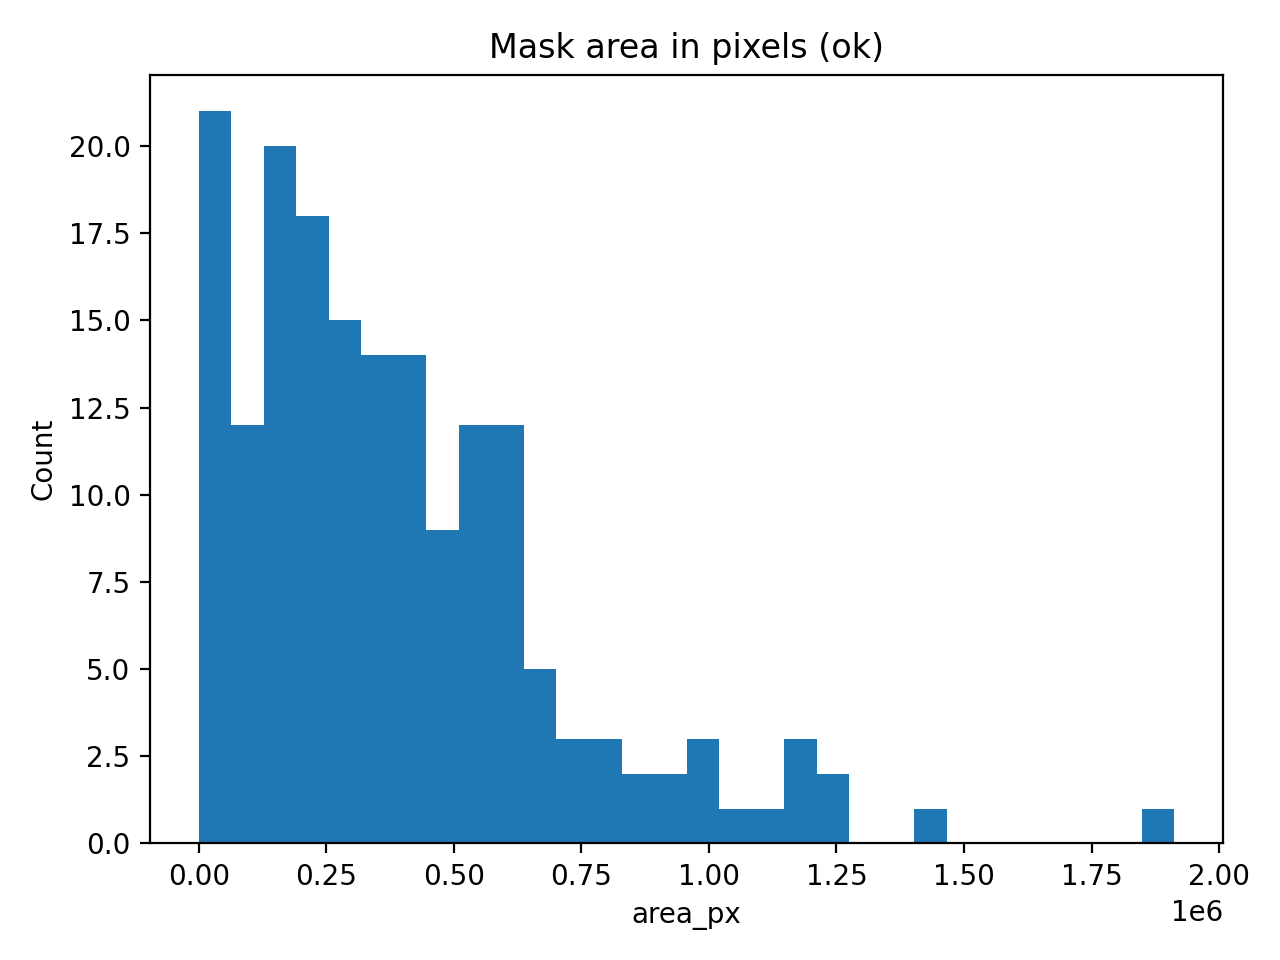
\includegraphics[width=\linewidth]{area_px_hist.png}
\caption*{(b) Mask area (pixels) distribution.}
\end{minipage}
\caption{Additional optimizer output diagnostics across all images (OK runs).}
\label{fig:appendix_optimizer_outputs}
\end{figure*}

\begin{figure*}[!t]
\centering
\begin{minipage}[b]{0.32\textwidth}\centering
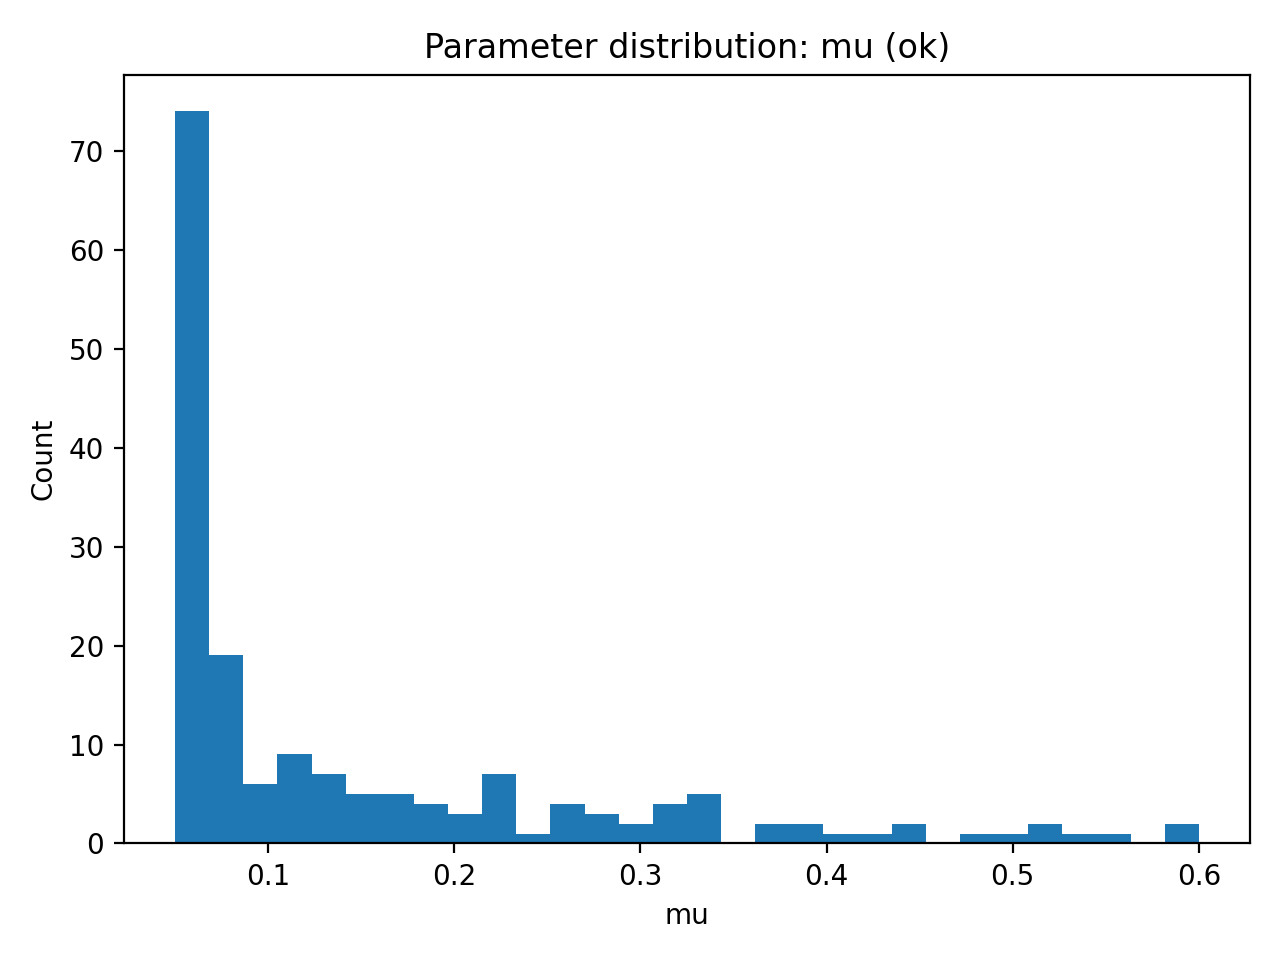
\includegraphics[width=\linewidth]{param_mu_hist.png}\caption*{(a) $\mu$}\end{minipage}\hfill
\begin{minipage}[b]{0.32\textwidth}\centering
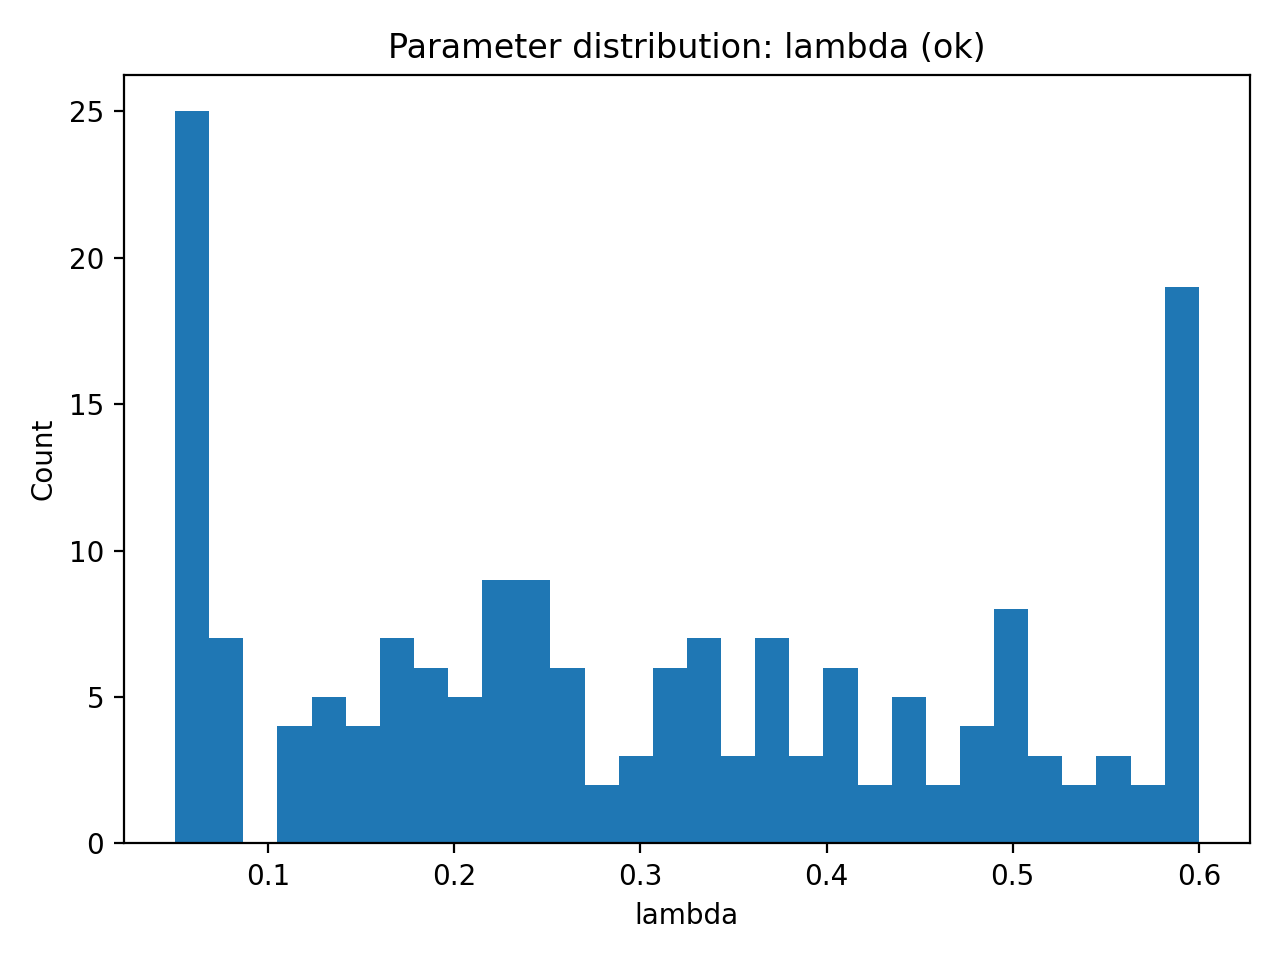
\includegraphics[width=\linewidth]{param_lambda_hist.png}\caption*{(b) $\lambda$}\end{minipage}\hfill
\begin{minipage}[b]{0.32\textwidth}\centering
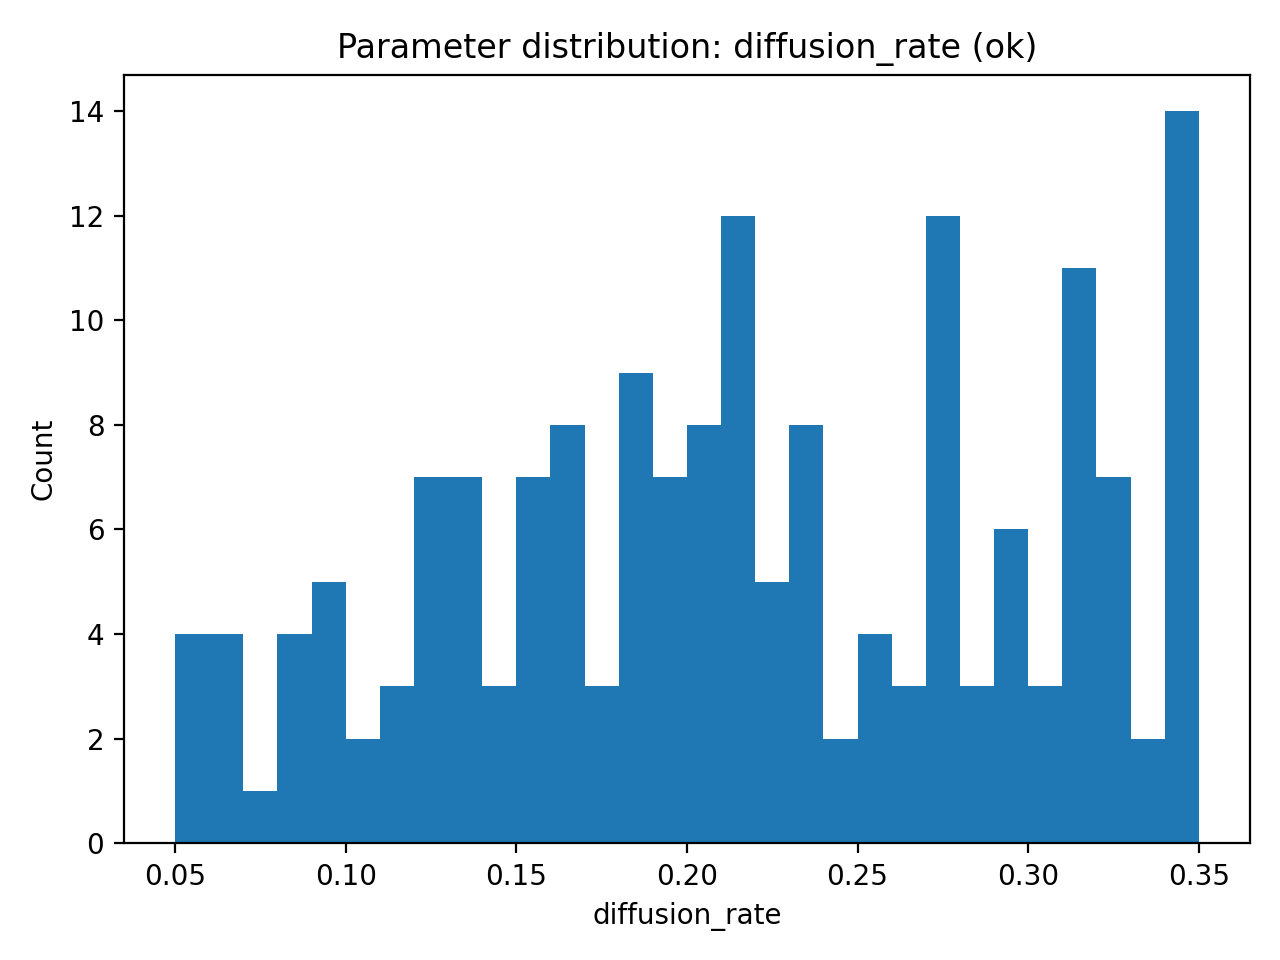
\includegraphics[width=\linewidth]{param_diffusion_rate_hist.png}\caption*{(c) diffusion}\end{minipage}

\vspace{2mm}

\begin{minipage}[b]{0.32\textwidth}\centering
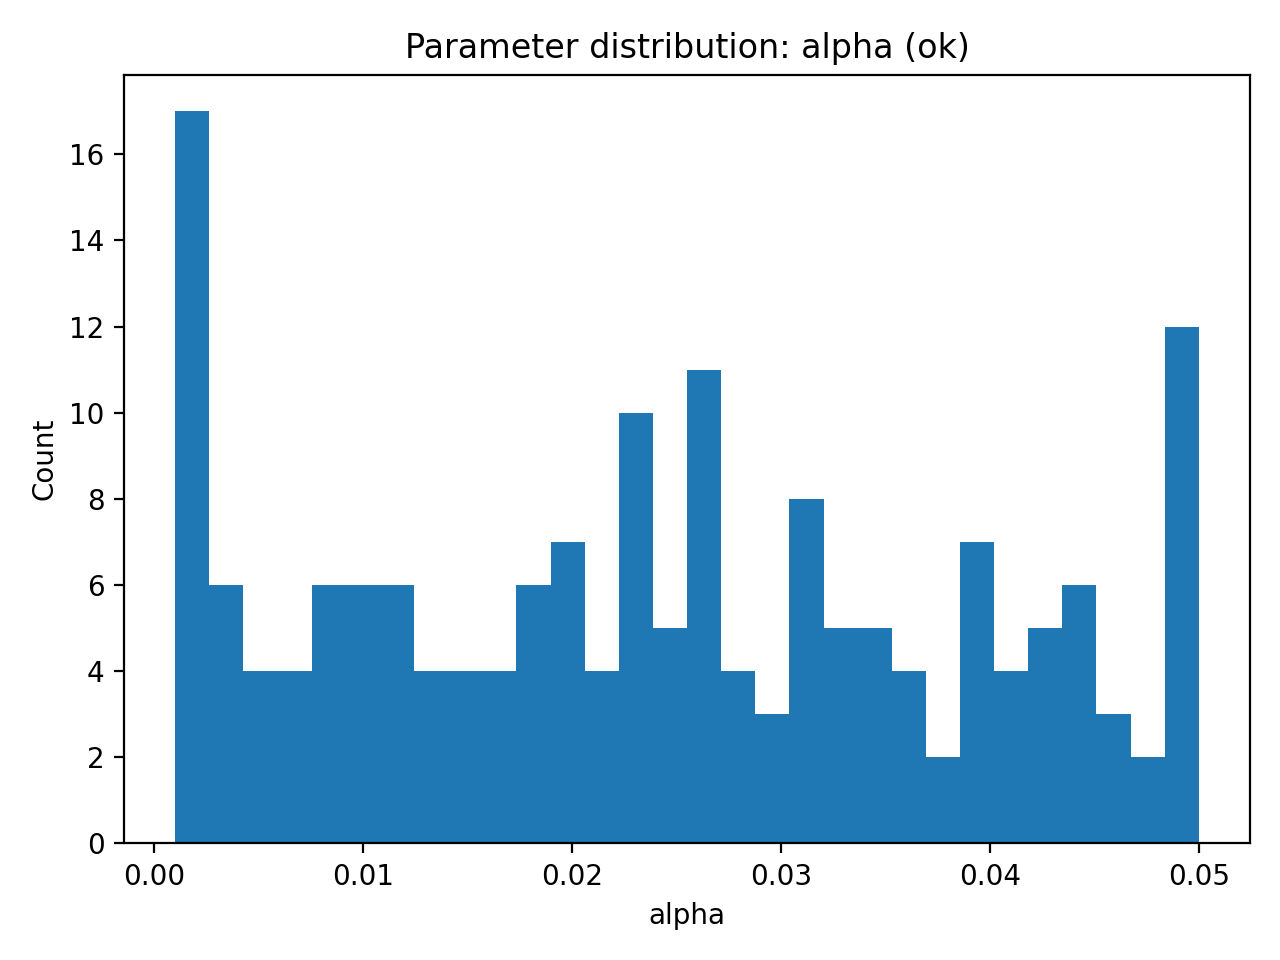
\includegraphics[width=\linewidth]{param_alpha_hist.png}\caption*{(d) $\alpha$}\end{minipage}\hfill
\begin{minipage}[b]{0.32\textwidth}\centering
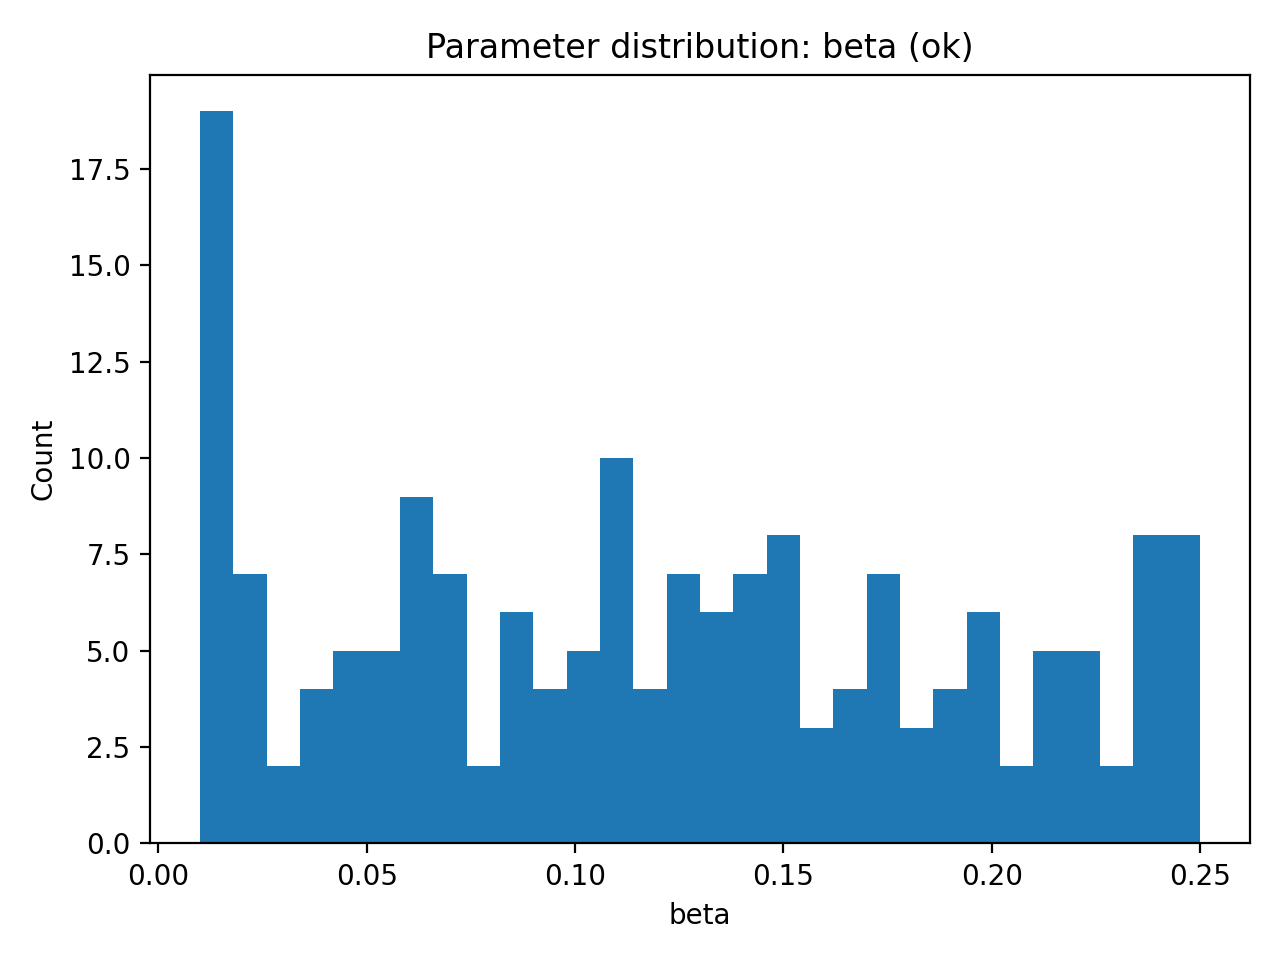
\includegraphics[width=\linewidth]{param_beta_hist.png}\caption*{(e) $\beta$}\end{minipage}\hfill
\begin{minipage}[b]{0.32\textwidth}\centering
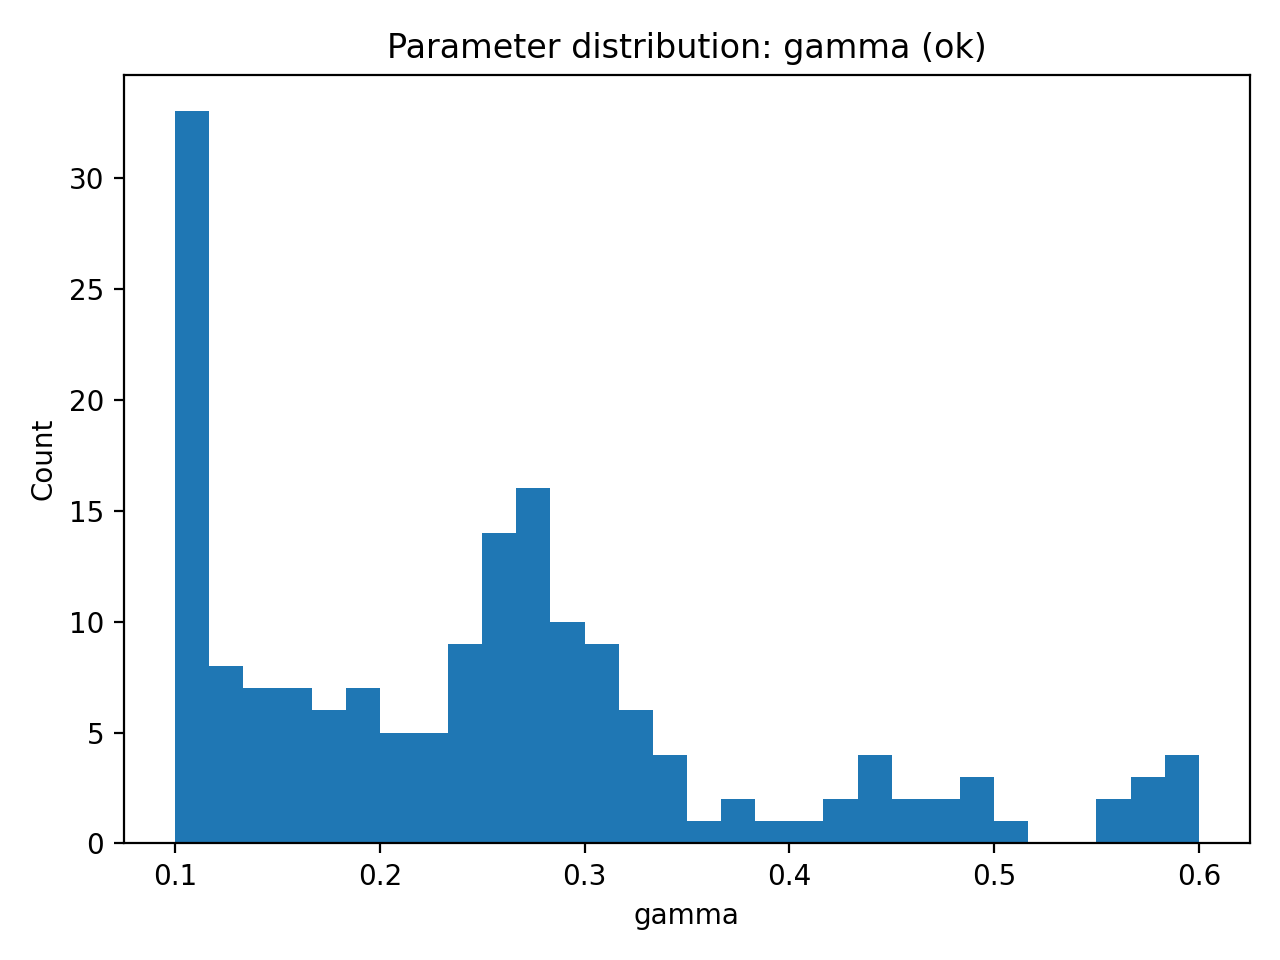
\includegraphics[width=\linewidth]{param_gamma_hist.png}\caption*{(f) $\gamma$}\end{minipage}

\vspace{2mm}

\begin{minipage}[b]{0.49\textwidth}\centering
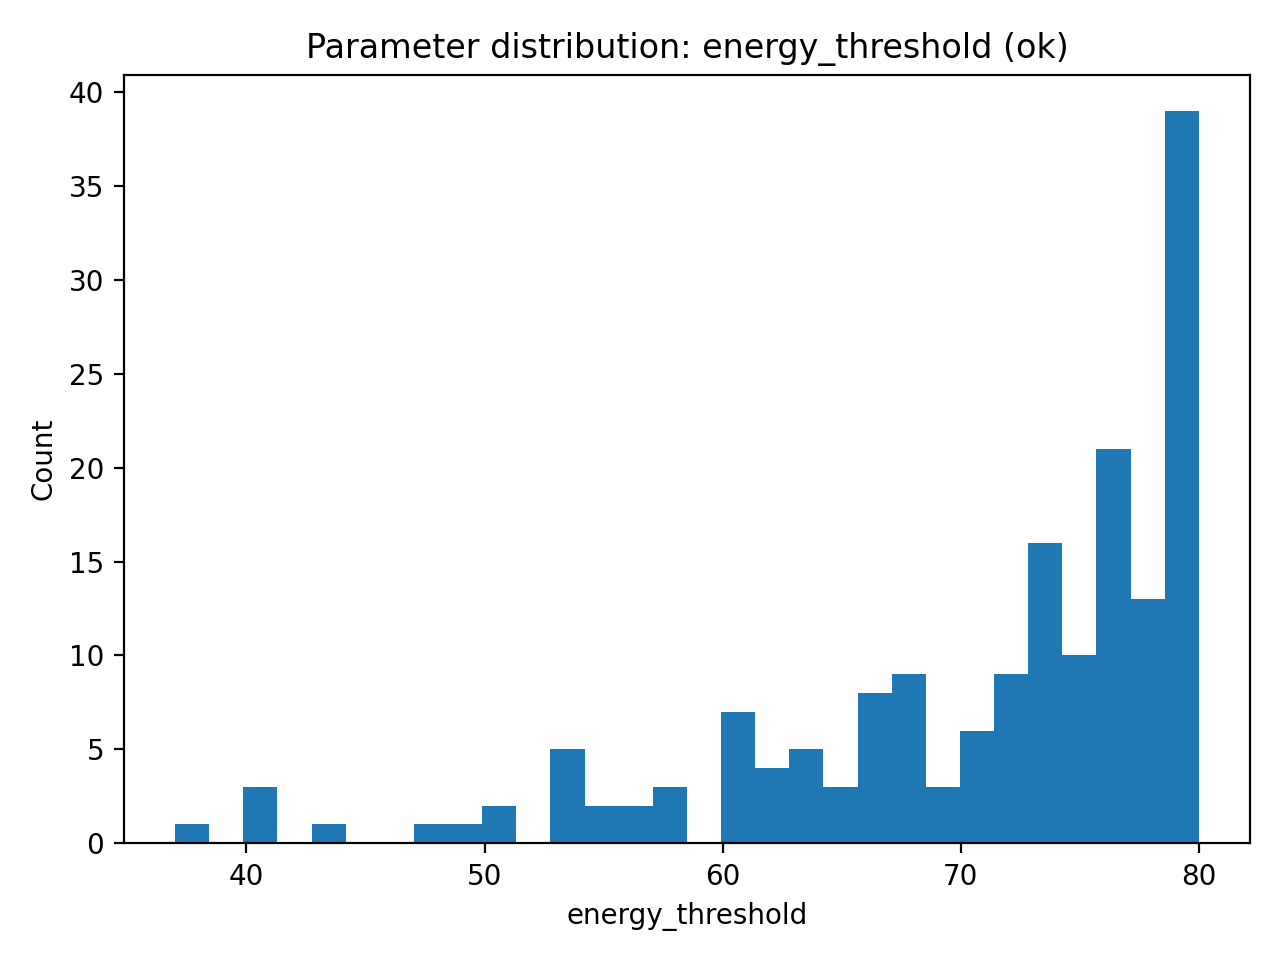
\includegraphics[width=\linewidth]{param_energy_threshold_hist.png}
\caption*{(g) $E_{\mathrm{thr}}$}\end{minipage}

\caption{Empirical distributions of optimized physics parameters across all images (OK runs).}
\label{fig:appendix_param_hists}
\end{figure*}

\section{Trace-Based Surface and Trajectory Supplementary Plots}
\label{sec:appendix_traces}
This section presents additional trace-based objective-surface and trajectory plots from the representative nine-leaf full-budget rerun. For each of the three score tiers (high, median, low), we show the convergence trajectory (best score so far vs.\ candidate index) and the search-region density ($T$--$\beta$ plane), providing further evidence for the landscape geometry findings in Section~\ref{sec:trace_analysis}.

\begin{figure*}[!t]
\centering
\begin{minipage}[b]{0.49\textwidth}
\centering
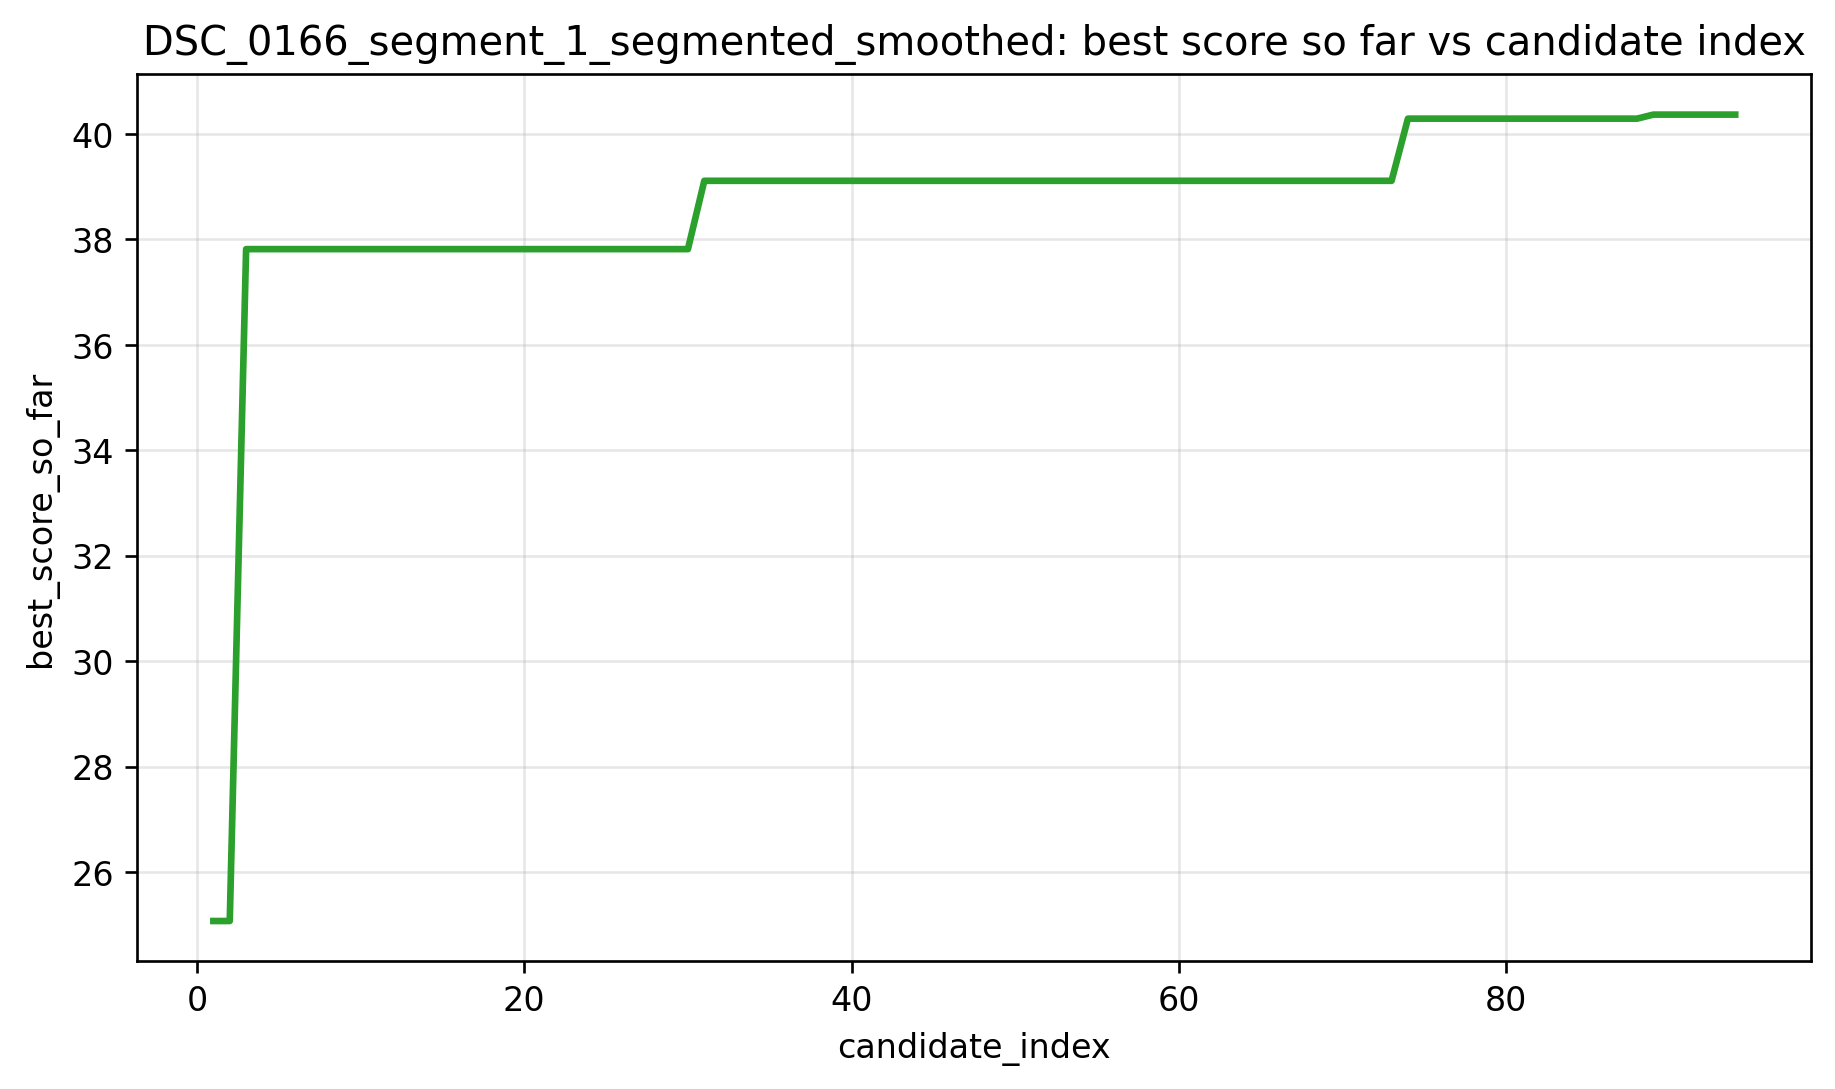
\includegraphics[width=\linewidth]{traj_DSC_0166_segment_1_segmented_smoothed__trajectory_best_score_so_far.png}
\caption*{(a) High-score leaf (DSC\_0166): convergence.}
\end{minipage}\hfill
\begin{minipage}[b]{0.49\textwidth}
\centering
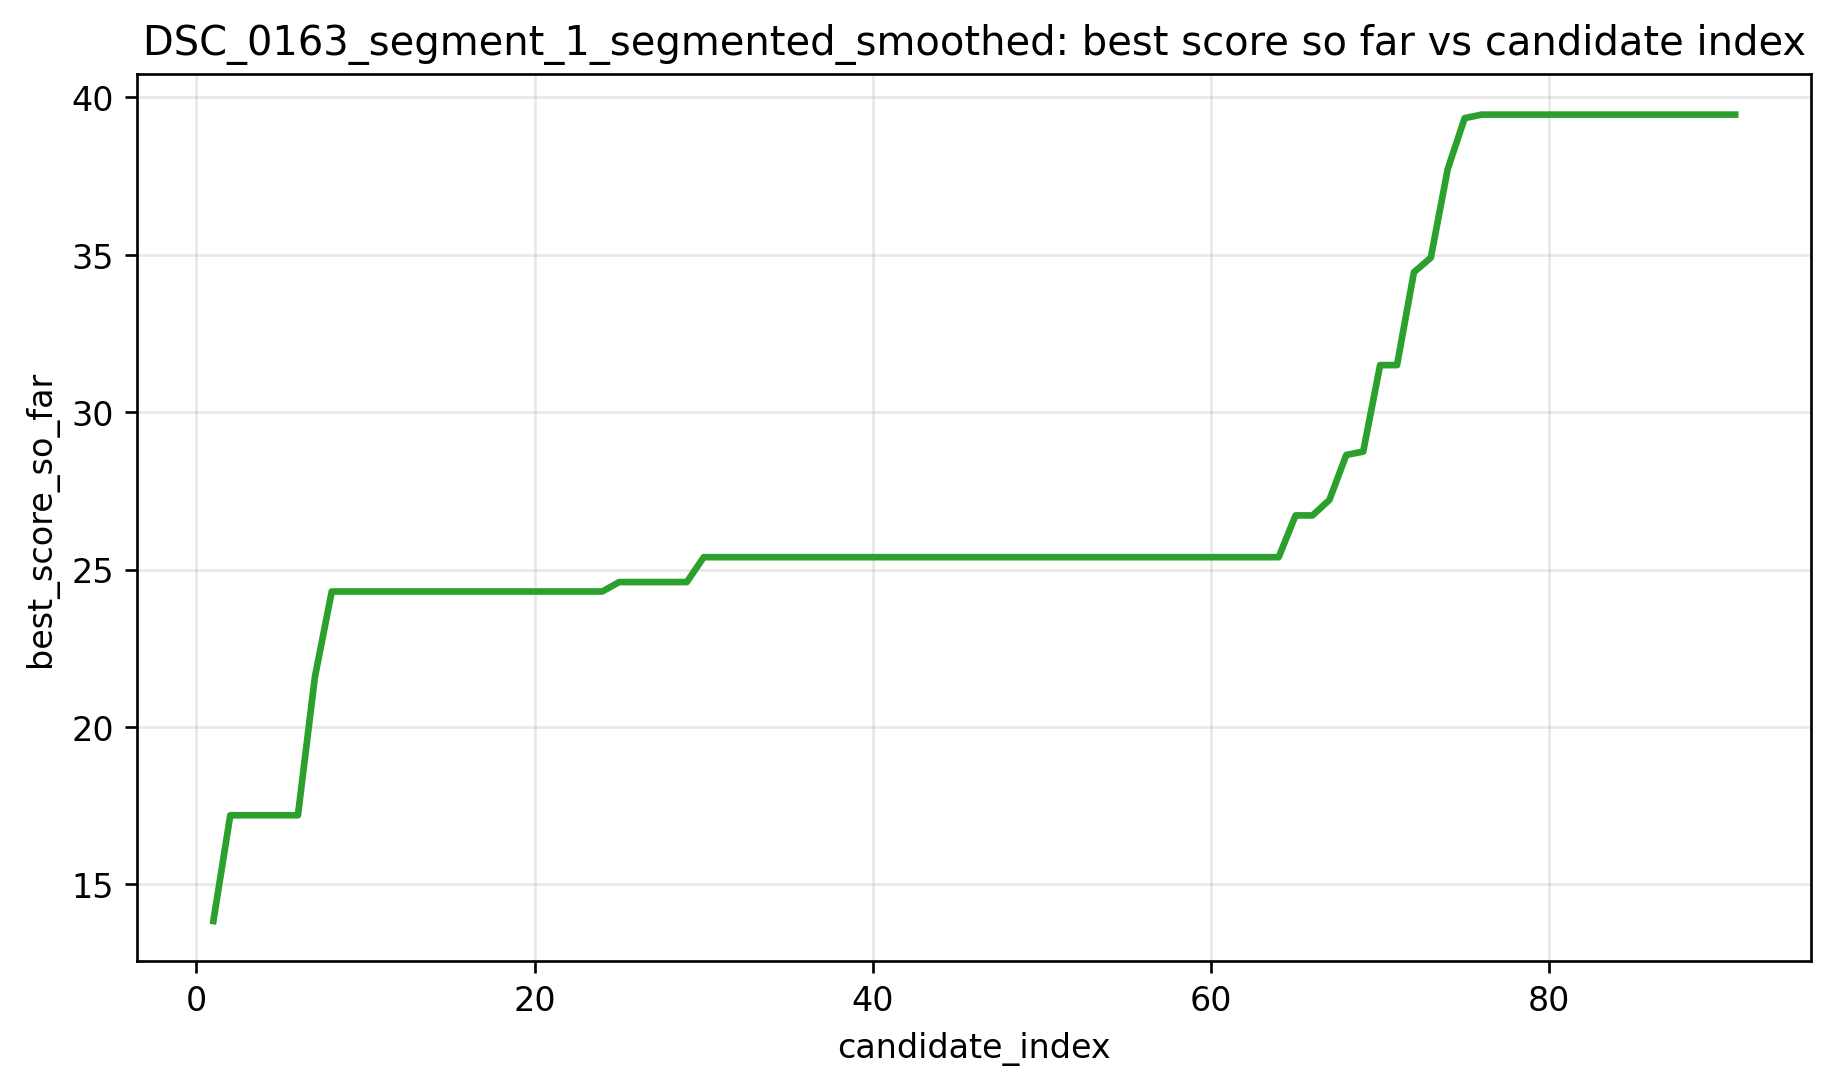
\includegraphics[width=\linewidth]{traj_DSC_0163_segment_1_segmented_smoothed__trajectory_best_score_so_far.png}
\caption*{(b) High-score leaf (DSC\_0163): convergence.}
\end{minipage}
\caption{Best-score-so-far convergence trajectories for additional high-score leaves.}
\label{fig:appendix_traj_high}
\end{figure*}

\begin{figure*}[!t]
\centering
\begin{minipage}[b]{0.49\textwidth}
\centering
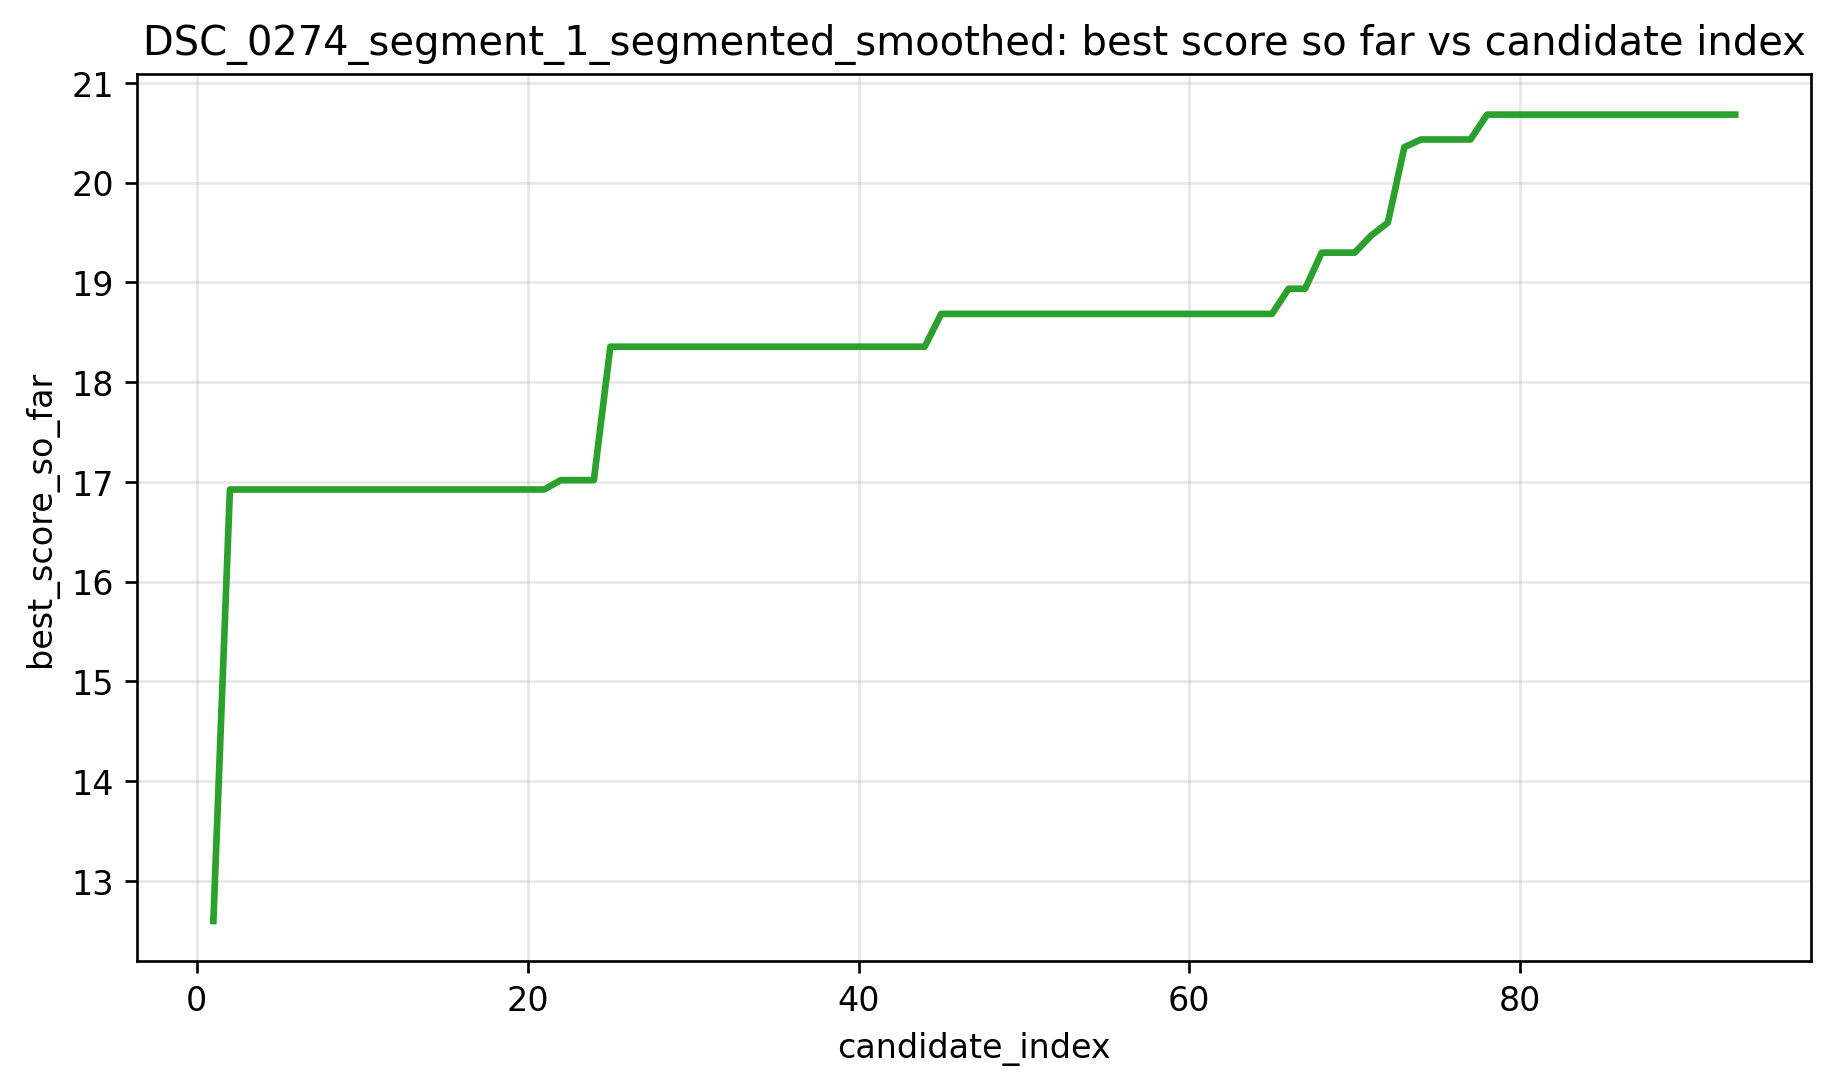
\includegraphics[width=\linewidth]{traj_DSC_0274_segment_1_segmented_smoothed__trajectory_best_score_so_far.png}
\caption*{(a) Median-score leaf (DSC\_0274): convergence.}
\end{minipage}\hfill
\begin{minipage}[b]{0.49\textwidth}
\centering
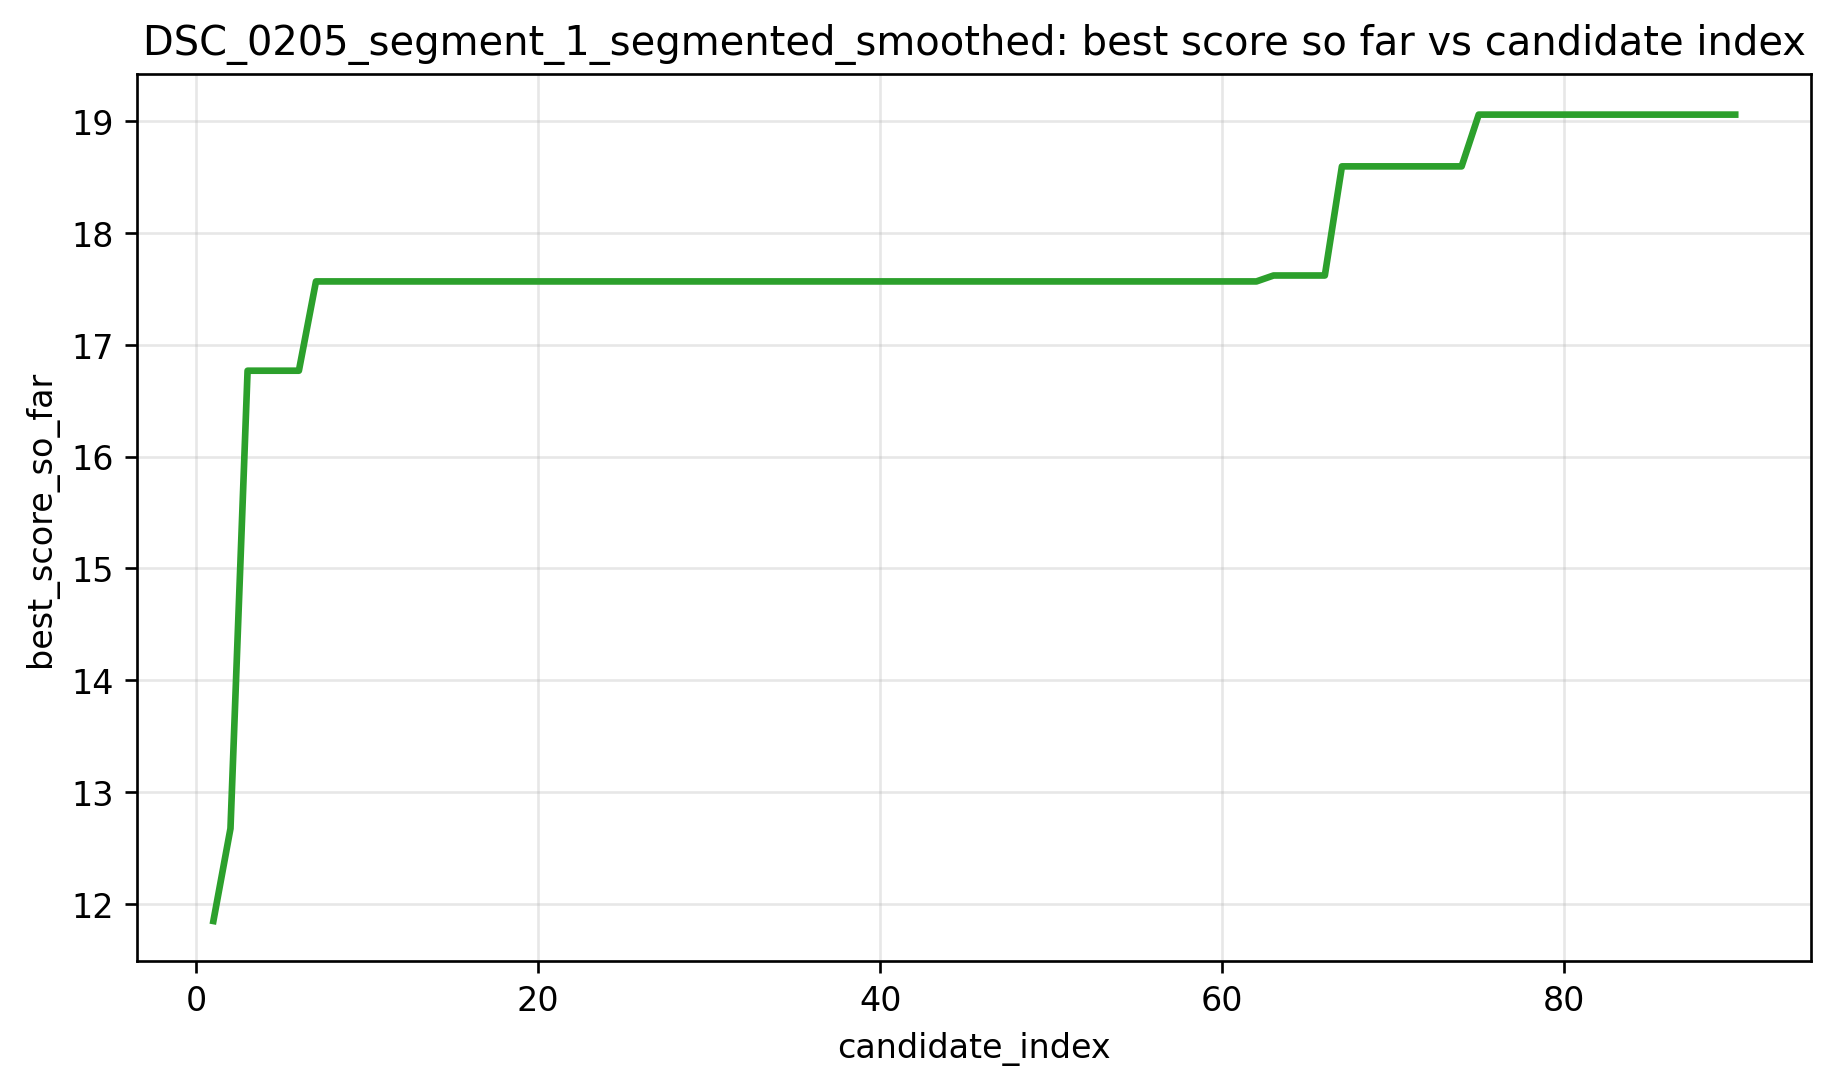
\includegraphics[width=\linewidth]{traj_DSC_0205_segment_1_segmented_smoothed__trajectory_best_score_so_far.png}
\caption*{(b) Median-score leaf (DSC\_0205): convergence.}
\end{minipage}
\caption{Best-score-so-far convergence trajectories for median-score leaves.}
\label{fig:appendix_traj_med}
\end{figure*}

\begin{figure*}[!t]
\centering
\begin{minipage}[b]{0.49\textwidth}
\centering
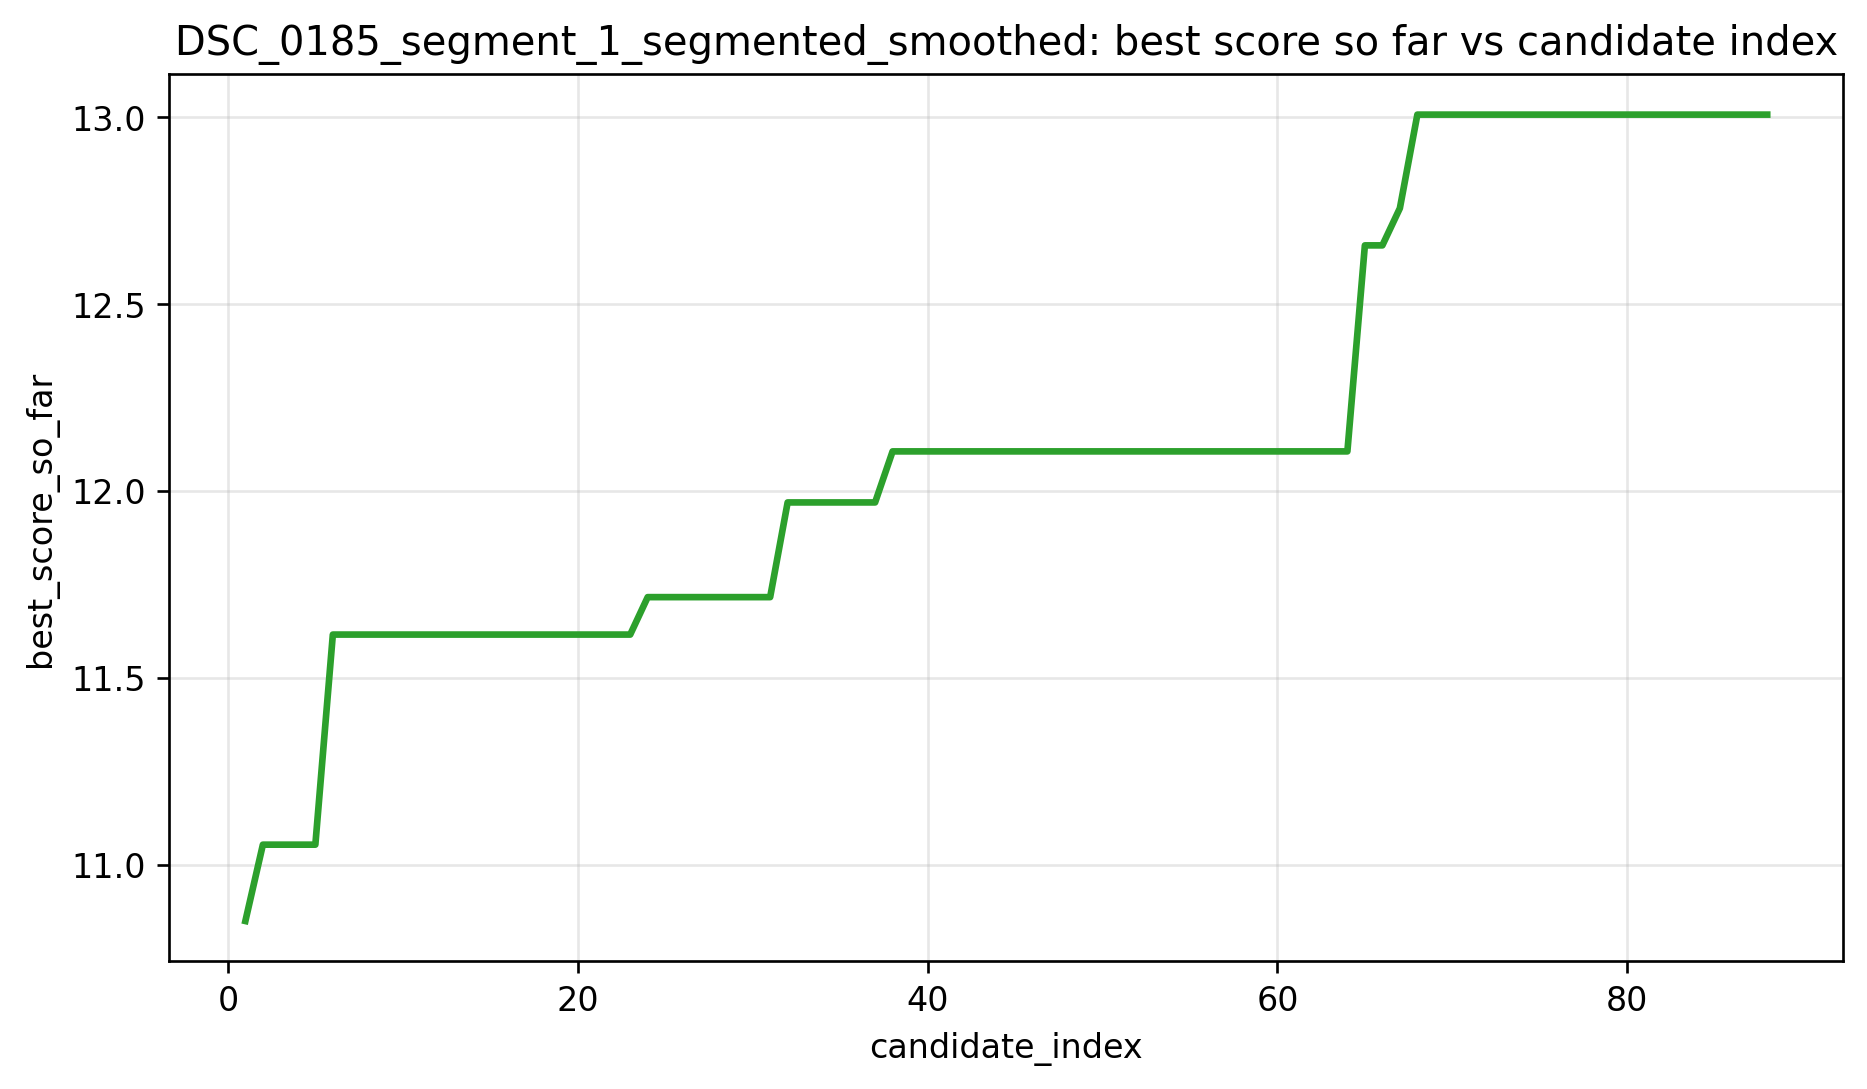
\includegraphics[width=\linewidth]{traj_DSC_0185_segment_1_segmented_smoothed__trajectory_best_score_so_far.png}
\caption*{(a) Low-score leaf (DSC\_0185): convergence.}
\end{minipage}\hfill
\begin{minipage}[b]{0.49\textwidth}
\centering
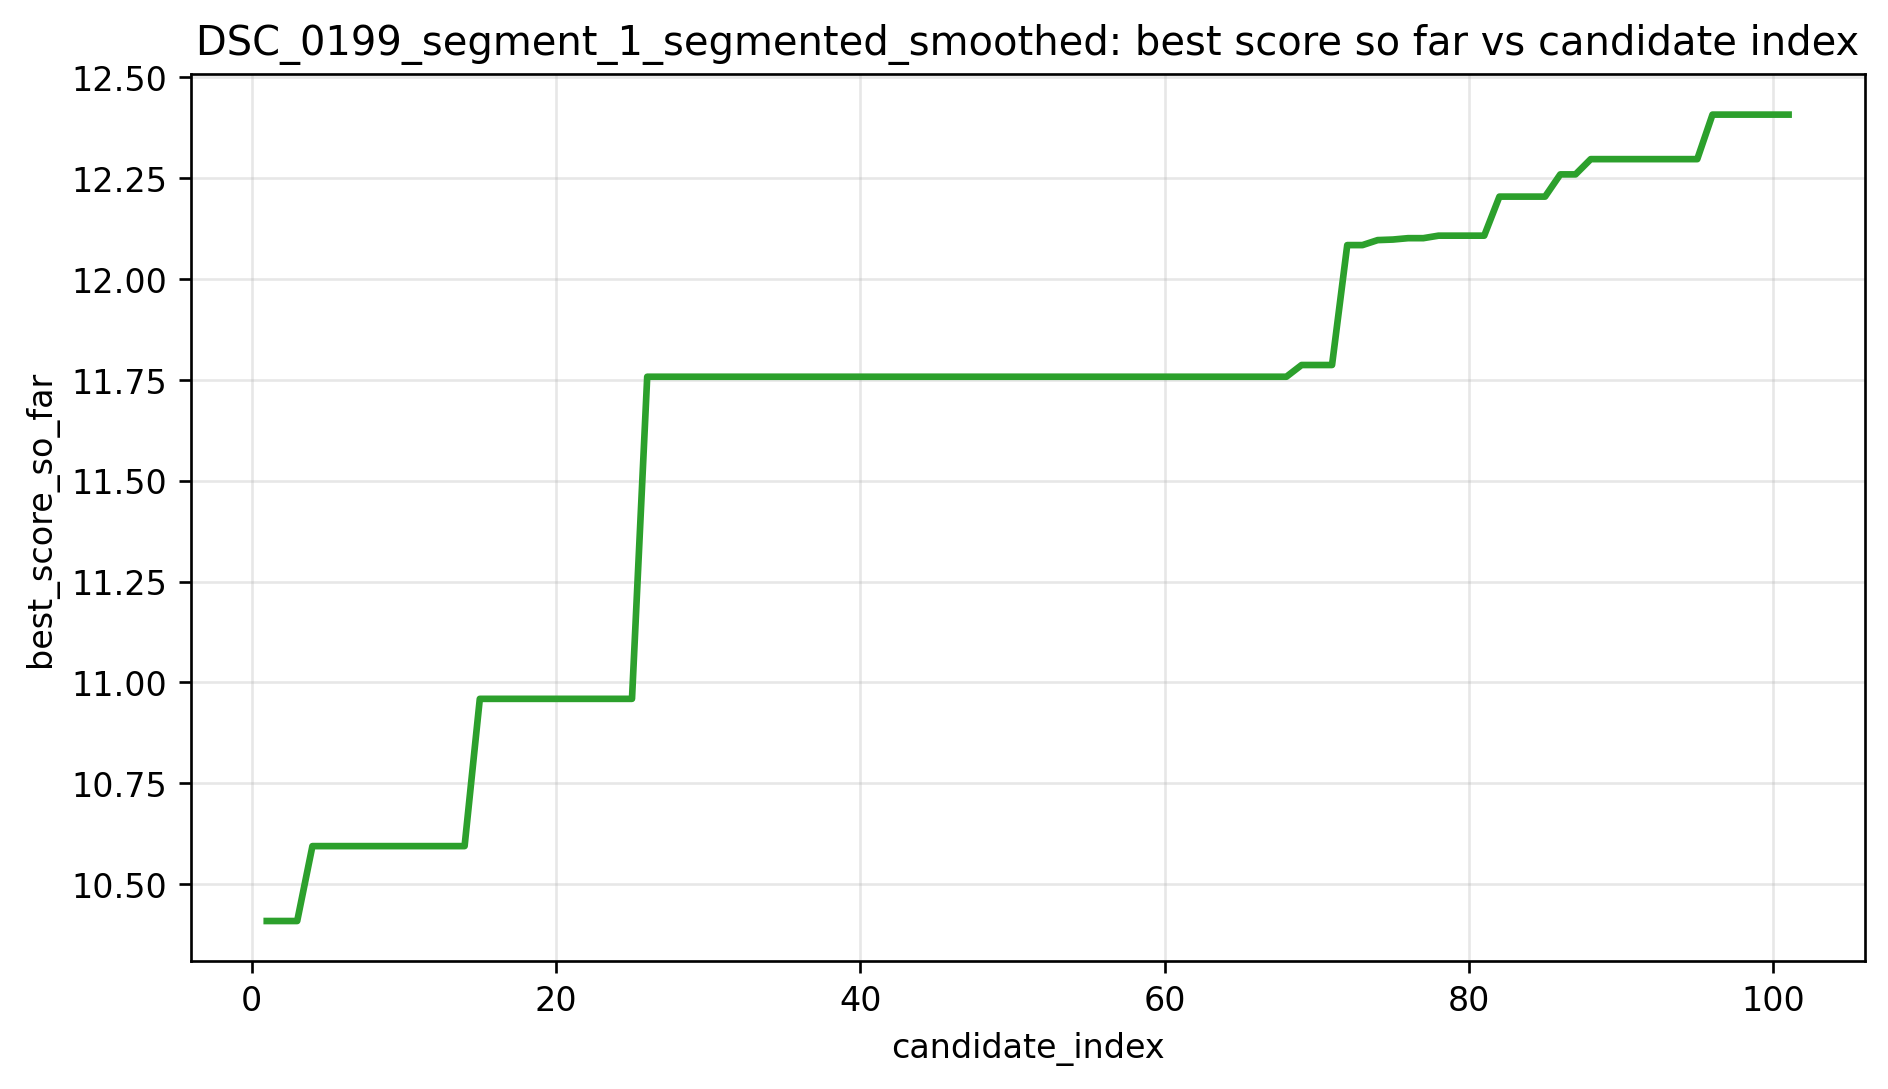
\includegraphics[width=\linewidth]{traj_DSC_0199_segment_1_segmented_smoothed__trajectory_best_score_so_far.png}
\caption*{(b) Low-score leaf (DSC\_0199): convergence.}
\end{minipage}
\caption{Best-score-so-far convergence trajectories for low-score leaves. Note the early plateau compared to high-score leaves.}
\label{fig:appendix_traj_low}
\end{figure*}

\section{Parameter-Cloud Geometry Supplementary Plots}
\label{sec:appendix_geometry}
This section presents additional parameter-cloud geometry plots from the manifold and solid-3D analyses described in Section~\ref{sec:param_geometry_results}.

\begin{figure*}[!t]
\centering
\begin{minipage}[b]{0.49\textwidth}
\centering
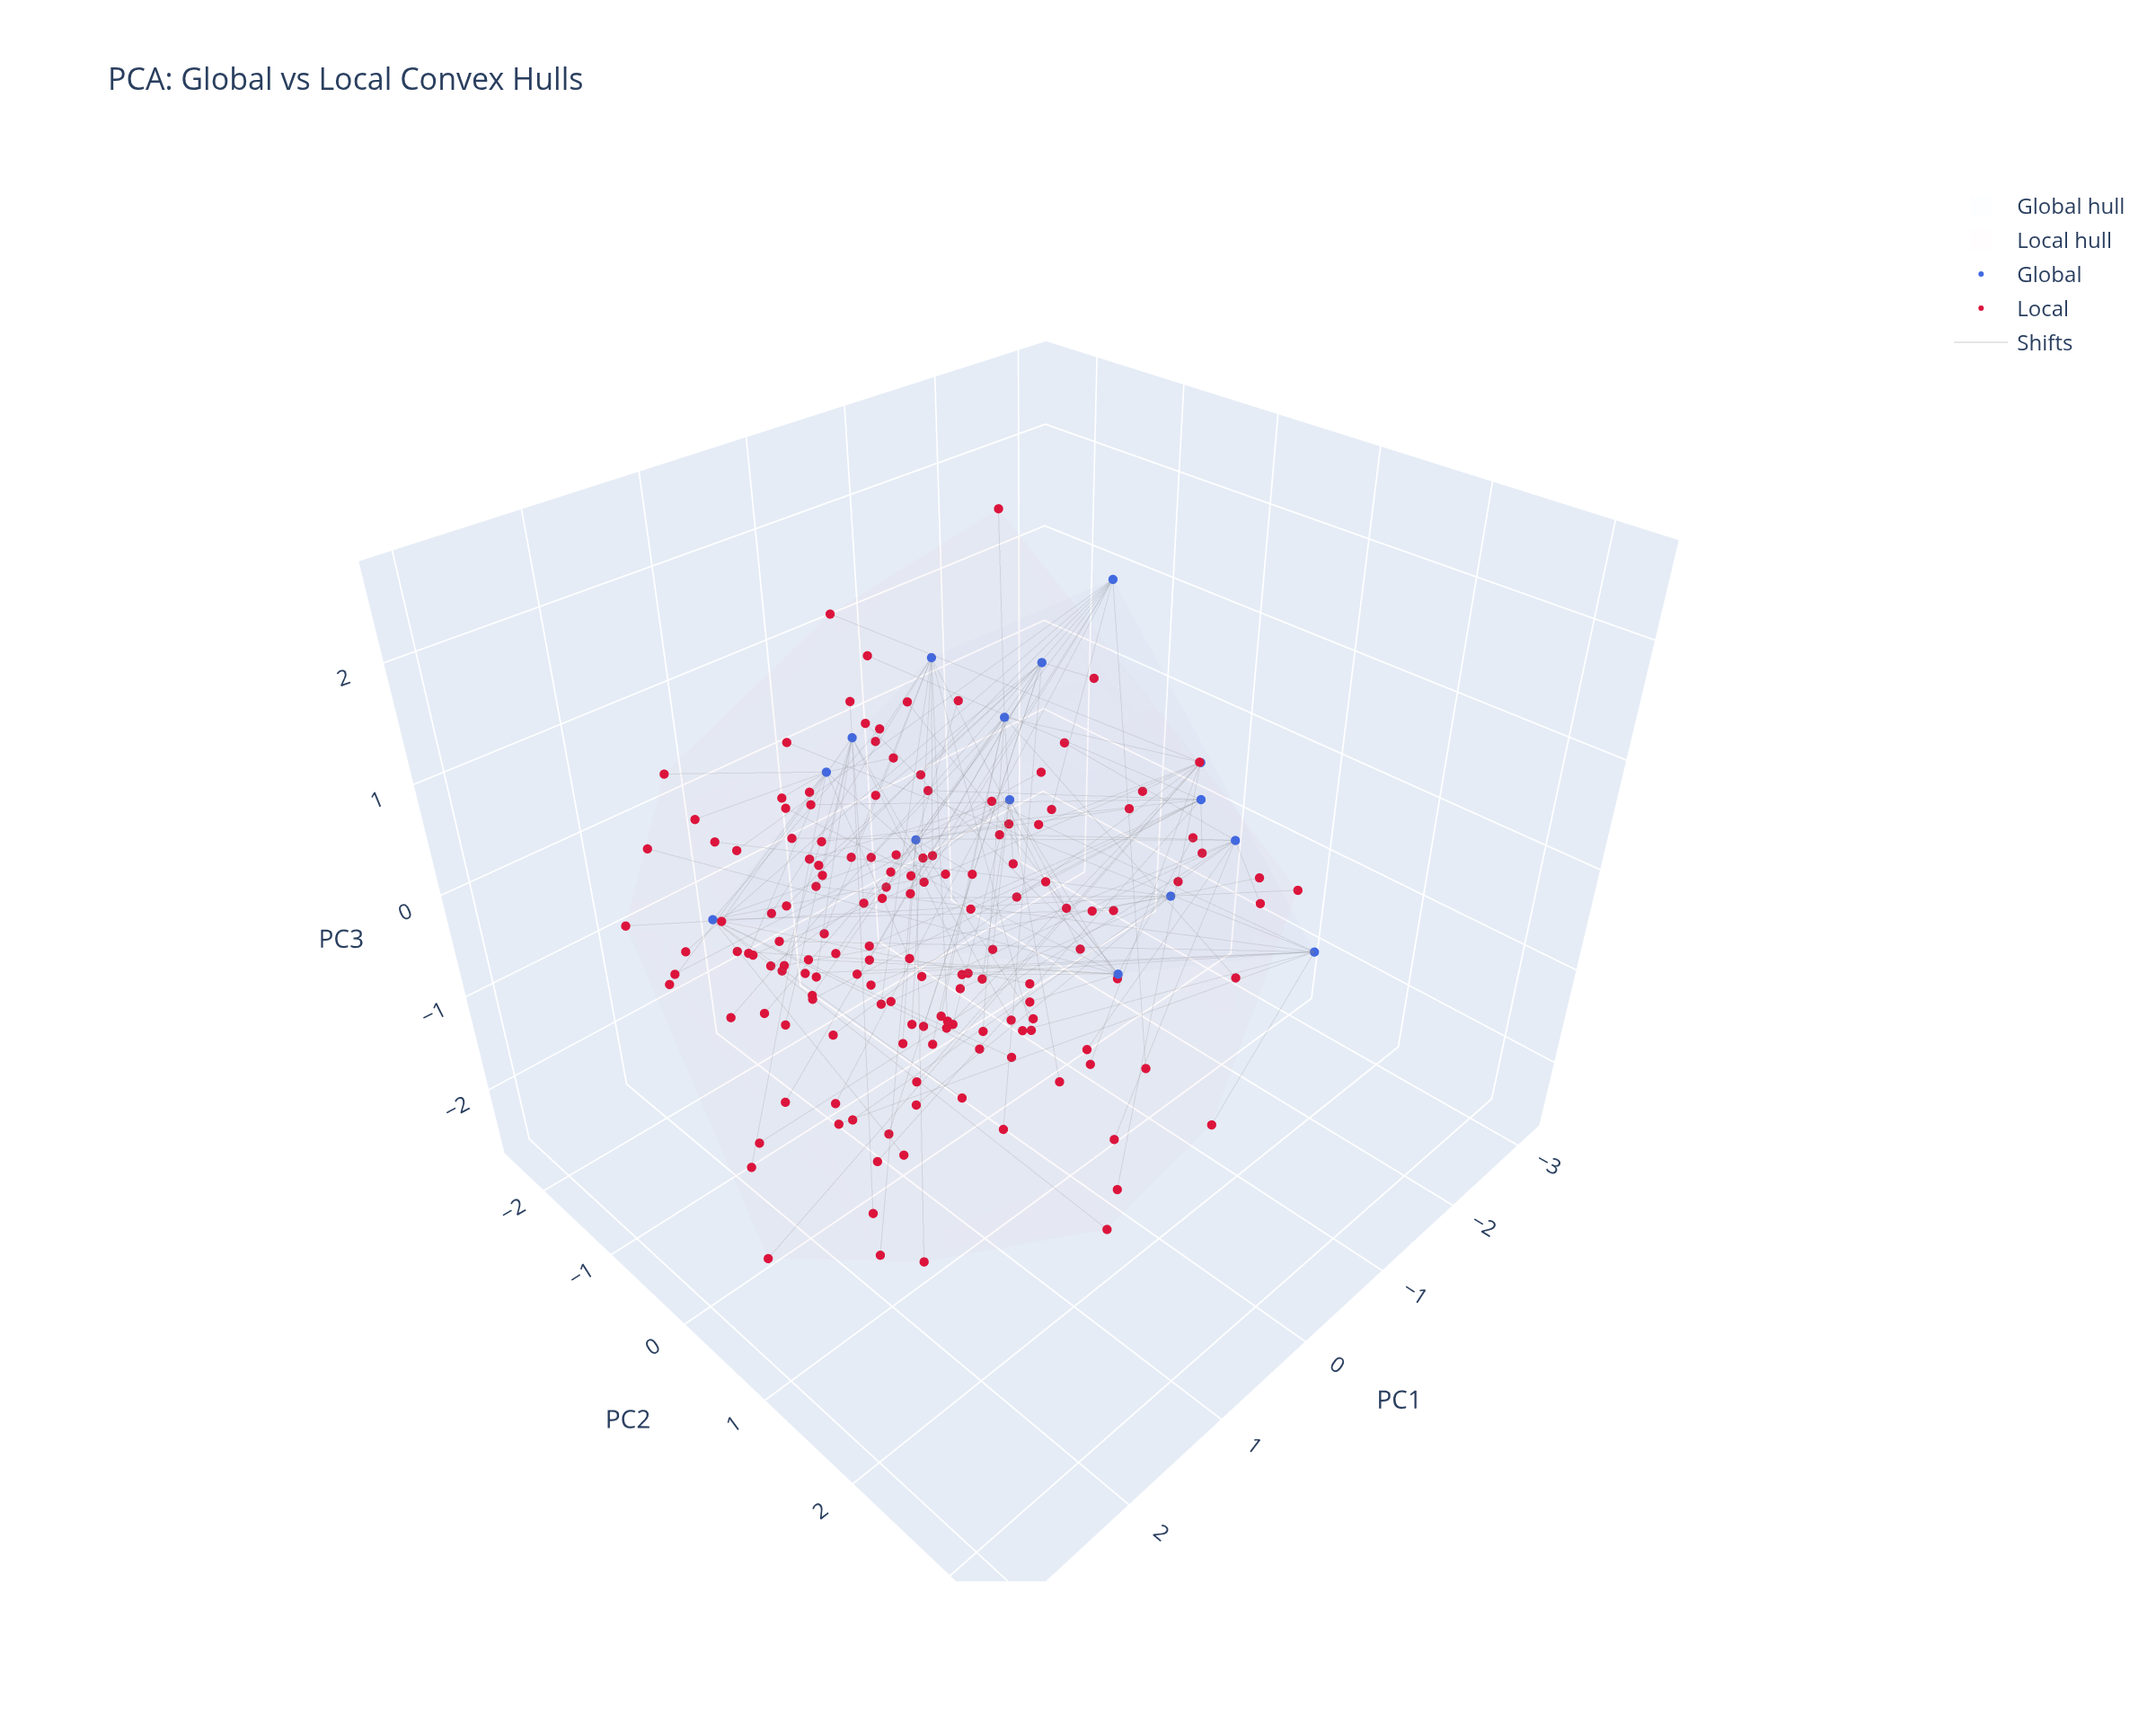
\includegraphics[width=\linewidth]{pca3d_convex_hull_global_local.png}
\caption*{(a) Convex hulls: global (blue) vs.\ local (red) in PCA space.}
\end{minipage}\hfill
\begin{minipage}[b]{0.49\textwidth}
\centering
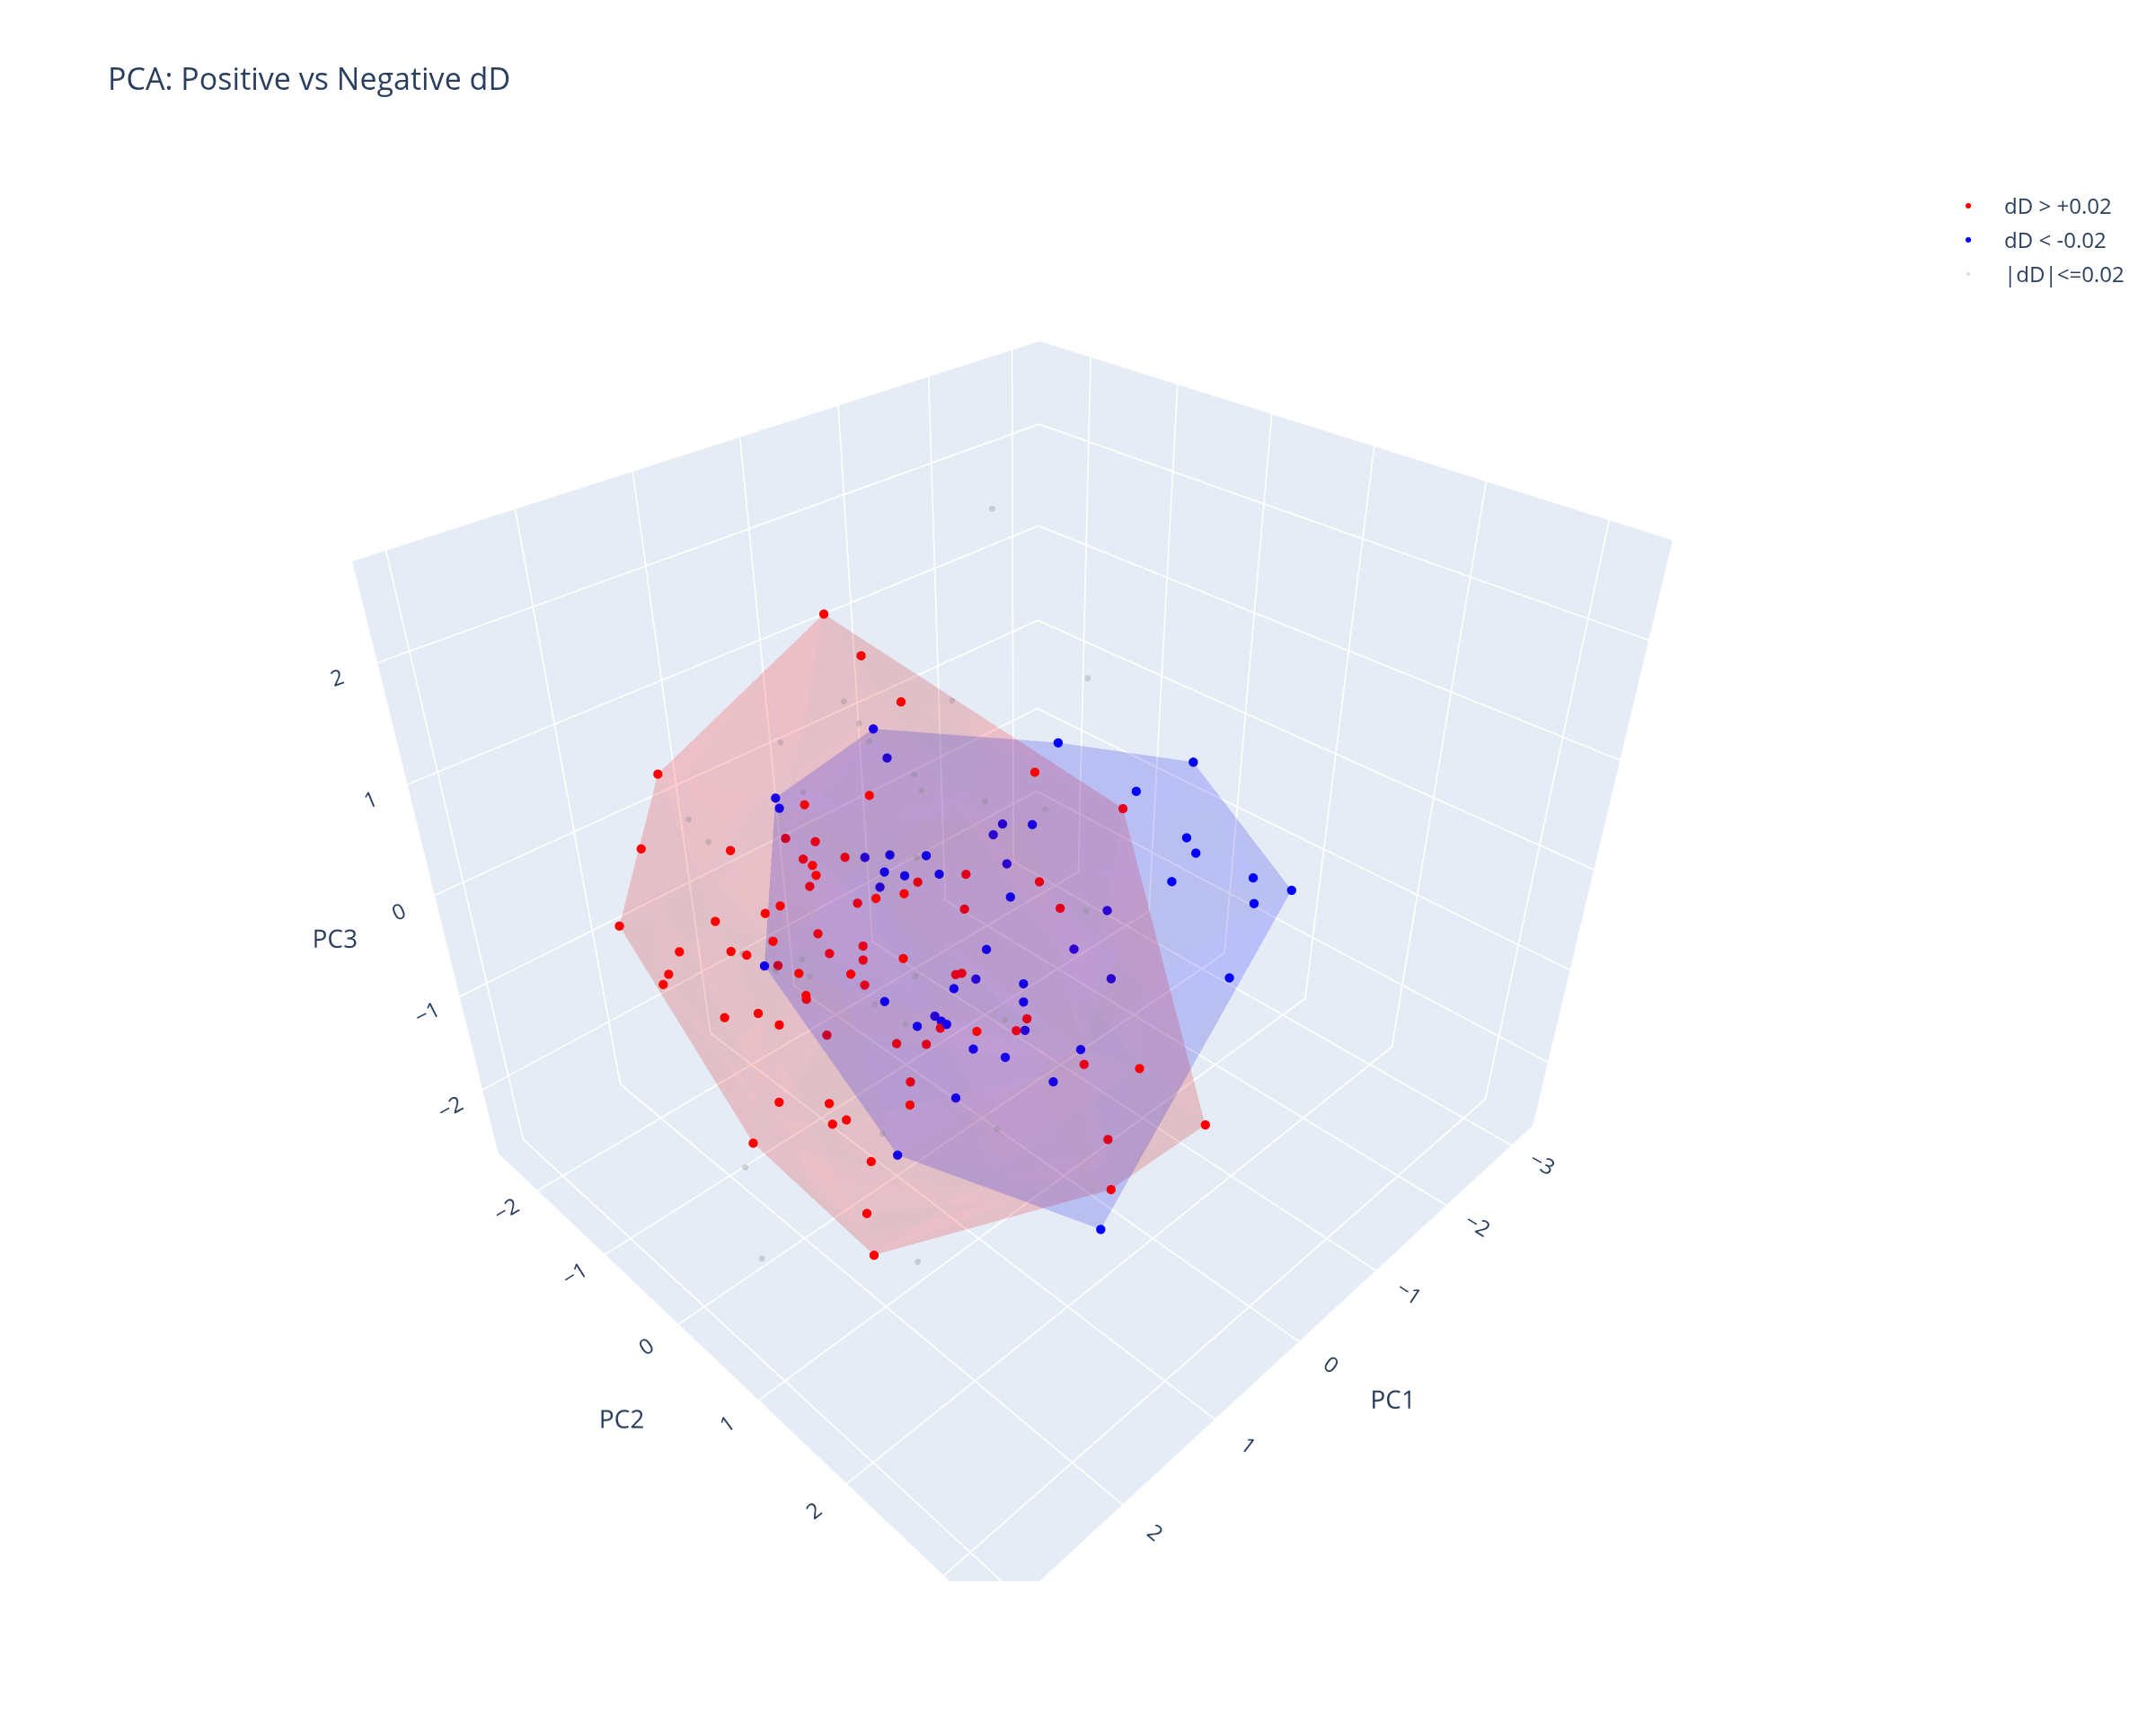
\includegraphics[width=\linewidth]{pca3d_positive_vs_negative_dD_surfaces.png}
\caption*{(b) Positive $\Delta D$ (red) vs.\ negative $\Delta D$ (blue) hulls.}
\end{minipage}
\caption{Supplementary solid-3D parameter geometry. (a) Convex hulls show the volumetric extent of global and local parameter clouds. (b) Separation of patches by Dice improvement sign reveals partial clustering of beneficial vs.\ detrimental local re-optimization in parameter space.}
\label{fig:appendix_solid3d}
\end{figure*}

\begin{figure*}[!t]
\centering
\begin{minipage}[b]{0.49\textwidth}
\centering
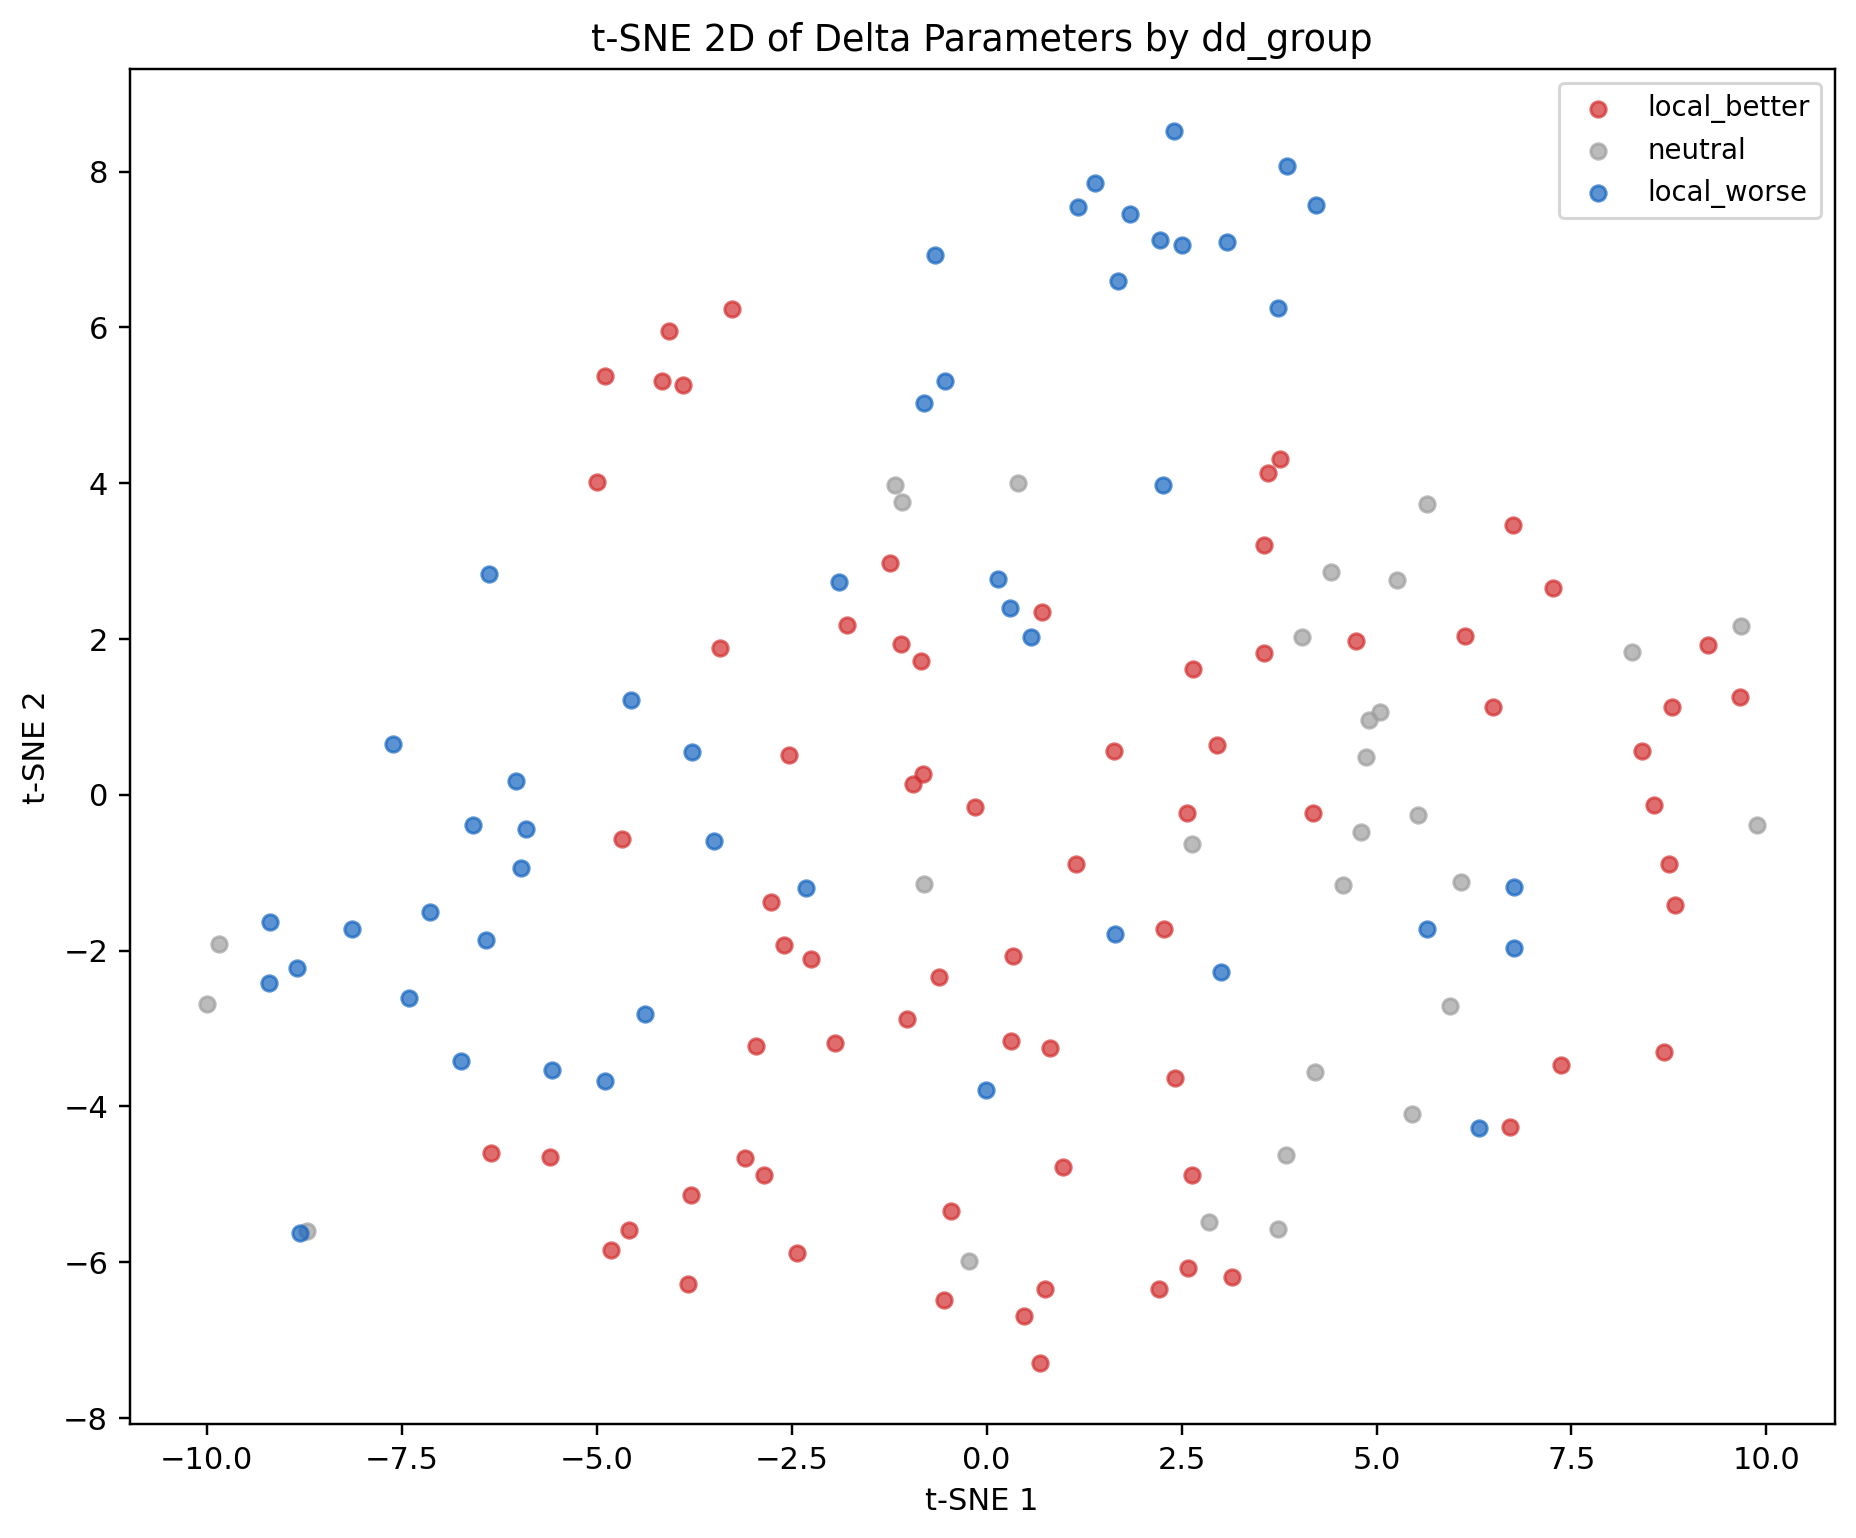
\includegraphics[width=\linewidth]{tsne2d_delta_ddgroup.png}
\caption*{(a) t-SNE of parameter shifts, colored by $\Delta D$ group.}
\end{minipage}\hfill
\begin{minipage}[b]{0.49\textwidth}
\centering
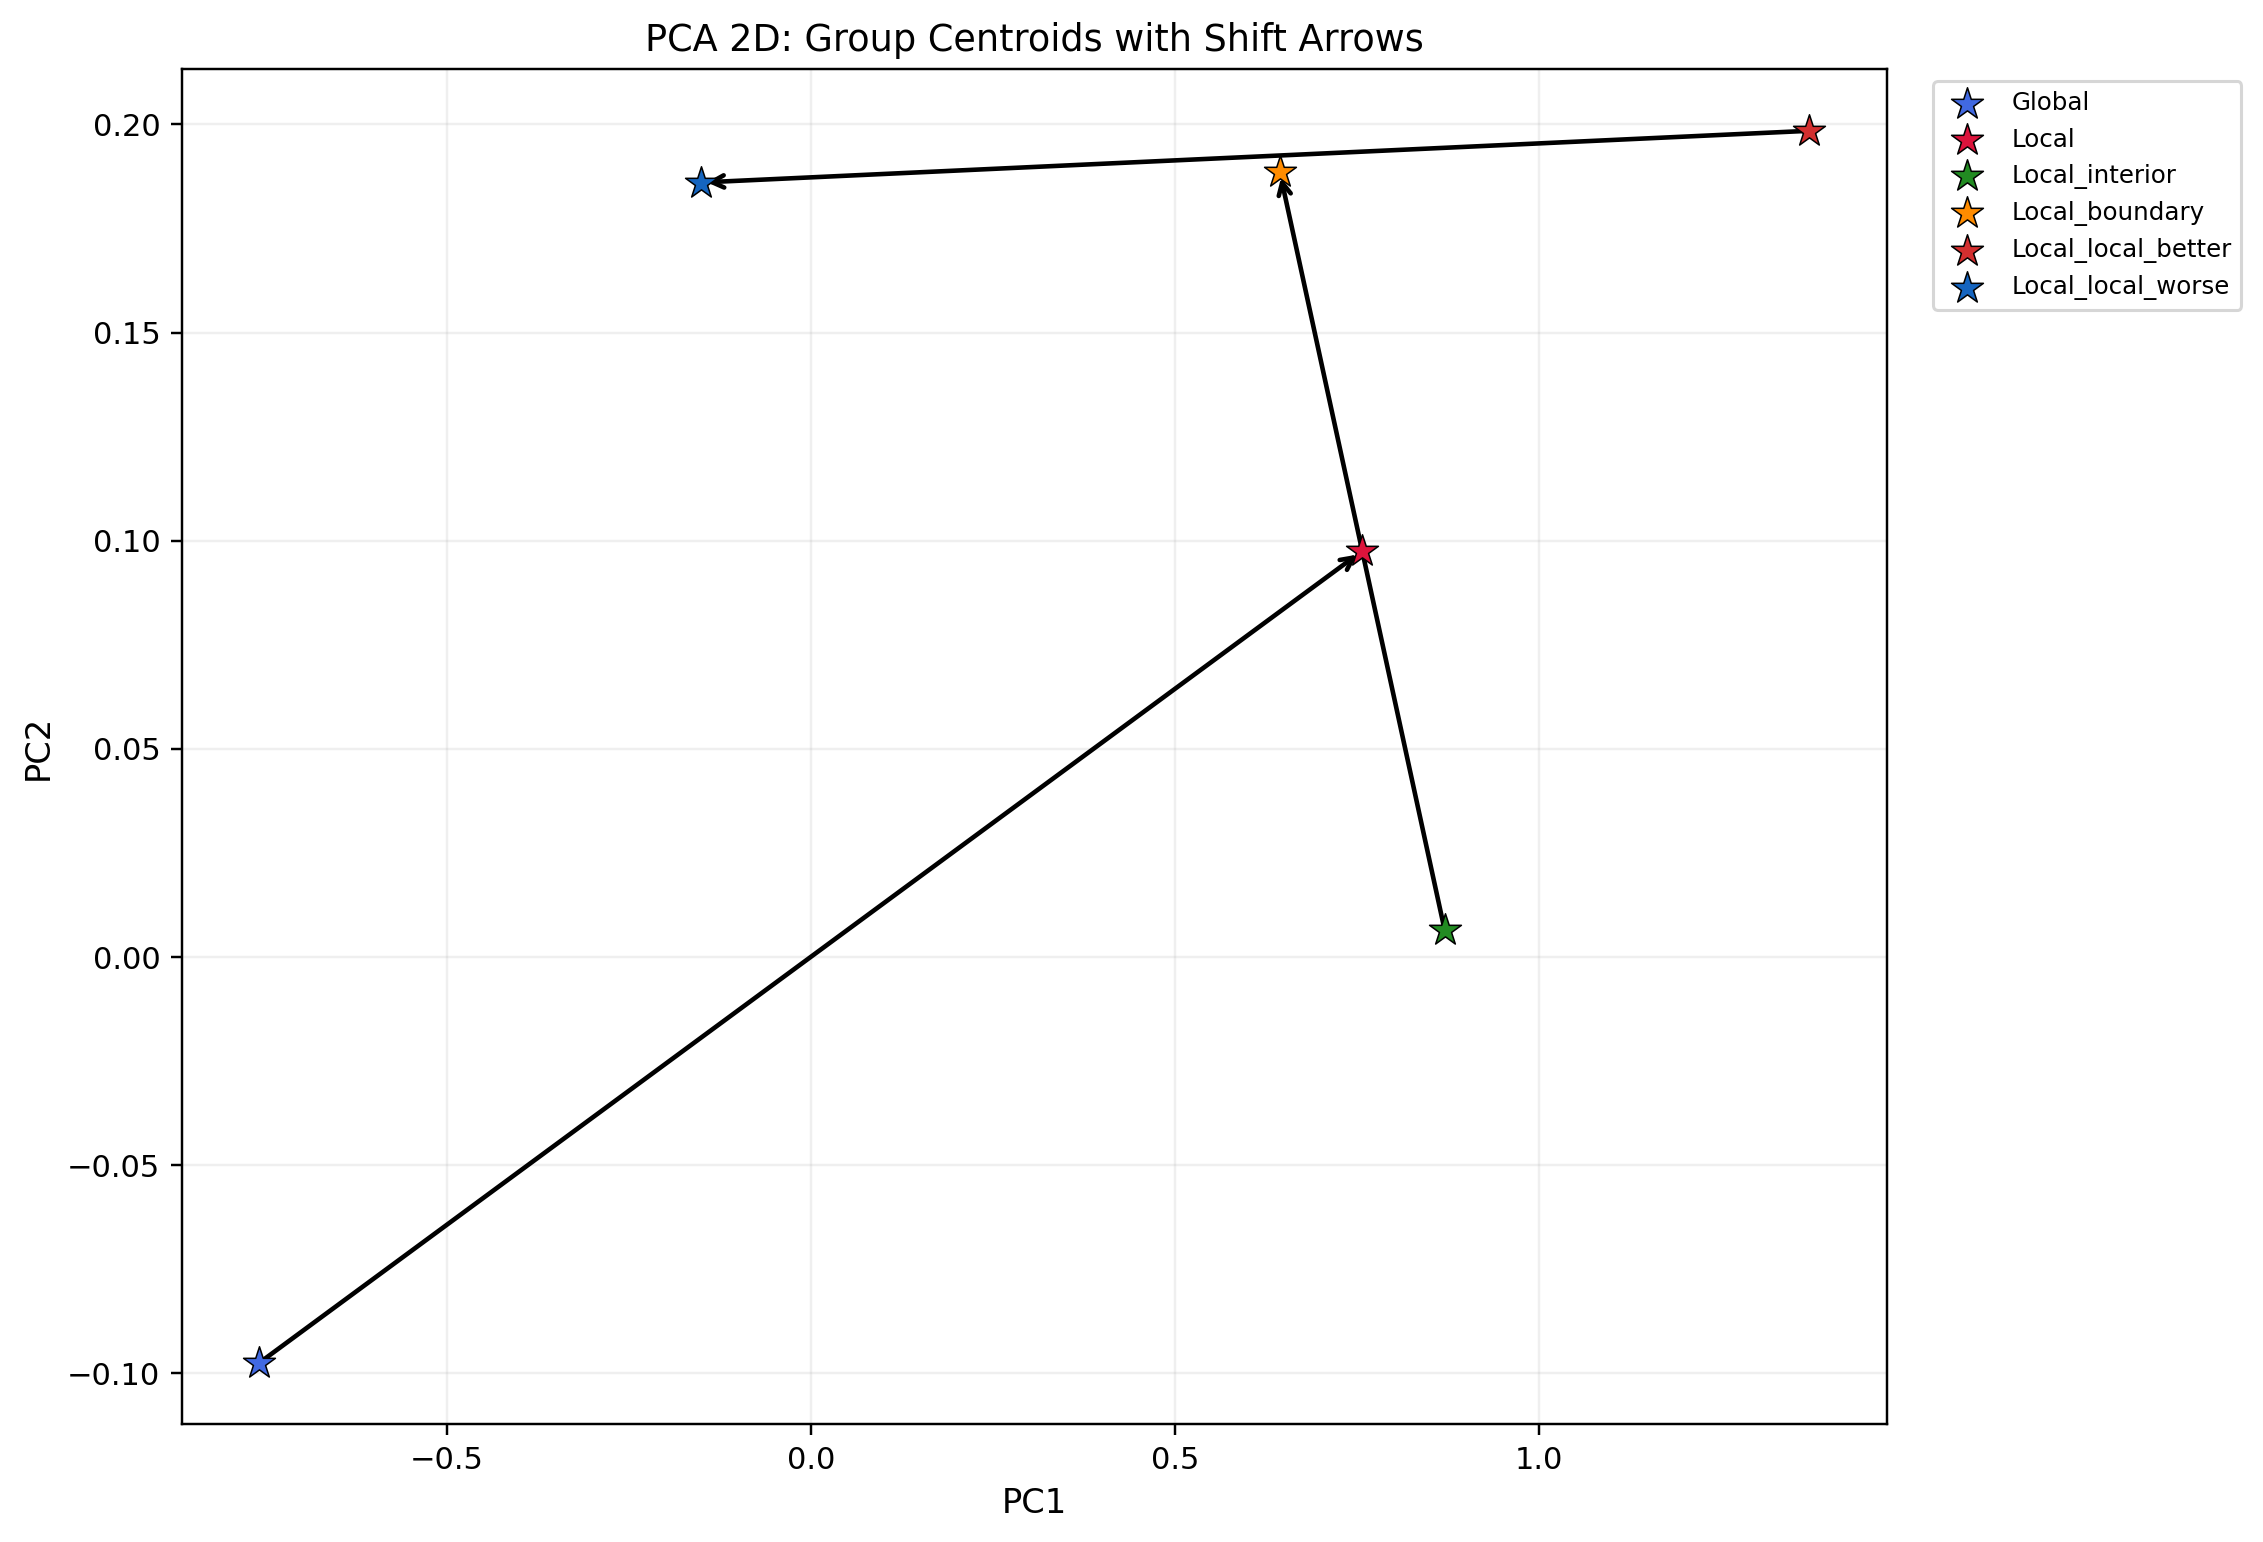
\includegraphics[width=\linewidth]{pca_centroid_shift_groups.png}
\caption*{(b) PCA centroid shift by $\Delta D$ group.}
\end{minipage}
\caption{Supplementary manifold embeddings. (a) t-SNE projection of delta-parameter vectors shows partial clustering of $\Delta D$ groups, confirming that the shift direction carries predictive information. (b) Group-level centroid shifts in PCA space.}
\label{fig:appendix_manifold}
\end{figure*}

\clearpage
\bibliographystyle{plainnat}
\bibliography{../bibliography/refs}
\end{document}
